%%%%%%%%%%%%%%%%%%%%%%% file template.tex %%%%%%%%%%%%%%%%%%%%%%%%%
%
% This is a general template file for the LaTeX package SVJour3
% for Springer journals.          Springer Heidelberg 2010/09/16
%
% Copy it to a new file with a new name and use it as the basis
% for your article. Delete % signs as needed.
%
% This template includes a few options for different layouts and
% content for various journals. Please consult a previous issue of
% your journal as needed.
%
%%%%%%%%%%%%%%%%%%%%%%%%%%%%%%%%%%%%%%%%%%%%%%%%%%%%%%%%%%%%%%%%%%%
%
% First comes an example EPS file -- just ignore it and
% proceed on the \documentclass line
% your LaTeX will extract the file if required
\begin{filecontents*}{example.eps}
%!PS-Adobe-3.0 EPSF-3.0
%%BoundingBox: 19 19 221 221
%%CreationDate: Mon Sep 29 1997
%%Creator: programmed by hand (JK)
%%EndComments
gsave
newpath
  20 20 moveto
  20 220 lineto
  220 220 lineto
  220 20 lineto
closepath
2 setlinewidth
gsave
  .4 setgray fill
grestore
stroke
grestore
\end{filecontents*}
%
\RequirePackage{fix-cm}
%
%\documentclass{svjour3}                     % onecolumn (standard format)
%\documentclass[smallcondensed]{svjour3}     % onecolumn (ditto)
%\documentclass[smallextended]{svjour3}       % onecolumn (second format)
\documentclass[twocolumn]{svjour3}          % twocolumn
%
\smartqed  % flush right qed marks, e.g. at end of proof
%
\usepackage{graphicx}
\usepackage{amssymb,amsmath}
\usepackage{verbatim,subfigure}
\usepackage{epsfig}
\usepackage{rotating}
\usepackage{flushend}
\usepackage{enumitem}
%\usepackage{color}
%\usepackage[usenames,dvipsnames]{color}
\usepackage[usenames,dvipsnames,svgnames,table]{xcolor}
\usepackage[pagebackref=true,breaklinks=true,colorlinks,linkcolor=OliveGreen,bookmarks=false,citecolor=blue]{hyperref}
\usepackage{soul}


% insert here the call for the packages your document requires
%\usepackage{latexsym}
% etc.
%
% please place your own definitions here and don't use \def but
\newcommand{\thl}[1]{\hl{#1}}

\newcommand{\V}[1] {\mathbf{#1}}
\newcommand{\Vx}[0] {\mathbf{x}}
\newcommand{\Vy}[0] {\mathbf{y}}
\newcommand{\Vz}[0] {\mathbf{z}}
\newcommand{\Vu}[0] {\mathbf{u}}
\newcommand{\Vv}[0] {\mathbf{v}}
\newcommand{\Vw}[0] {\mathbf{w}}

\newcommand{\Vb}[2] {\V{#1}_{#2}}
\newcommand{\Vxb}[1] {\Vx_{#1}}
\newcommand{\Vzb}[1] {\Vz_{#1}}
\newcommand{\Vxp}[1] {\Vx^{#1}}

\newcommand{\Vbp}[3] {\V{#1}_{#2}^{#3}}
\newcommand{\Vxbp}[2] {\Vx_{#1}^{#2}}
\newcommand{\Vzbp}[2] {\Vz_{#1}^{#2}}
\newcommand{\Vubp}[2] {\Vu_{#1}^{#2}}
\newcommand{\Vvbp}[2] {\Vv_{#1}^{#2}}
\newcommand{\Vwbp}[2] {\Vw_{#1}^{#2}}
\newcommand{\VSbp}[2] {\V{\Sigma}_{#1}^{#2}}
\newcommand{\dVxbp}[2] {\dot{\Vxbp{#1}{#2}}}

\newcommand{\pVbp}[4] {{}^{#1}\V{#2}_{#3}^{#4}}
\newcommand{\pVzb}[2] {{}^{#1}\Vz_{#2}}
\newcommand{\pVxbp}[3] {{}^{#1}\Vx_{#2}^{#3}}
\newcommand{\pVvbp}[3] {{}^{#1}\Vv_{#2}^{#3}}
\newcommand{\pVzbp}[3] {{}^{#1}\Vz_{#2}^{#3}}
\newcommand{\ptVzbp}[3] {{}^{#1}\tilde \Vz_{#2}^{#3}}
\newcommand{\ptVzb}[2] {{}^{#1}\tilde\Vz_{#2}}
\newcommand{\tVxp}[1] {\tilde \Vx^{#1}}
\newcommand{\tVxbp}[2] {\tilde \Vx_{#1}^{#2}}
\newcommand{\tVzbp}[2] {\tilde \Vz_{#1}^{#2}}
\newcommand{\tVubp}[2] {\tilde \Vu_{#1}^{#2}}
\newcommand{\tVzb}[1] {\tilde \Vz_{#1}}
\newcommand{\mVxbp}[2] {\bar \Vx_{#1}^{#2}}
\newcommand{\pmVxbp}[3] {{}^{#1}\bar \Vx_{#2}^{#3}}
\newcommand{\bpVp}[4] {{}_{#1}^{#2}\V{#3}^{#4}}

\newcommand{\Sz}[0] {z}
\newcommand{\tSzbp}[2] {\tilde \Sz_{#1}^{#2}}
\newcommand{\ptSzbp}[3] {{}^{#1}\tilde \Sz_{#2}^{#3}}

\newcommand{\sbram}[1] {\left \{ #1 \right .}
\newcommand{\vm}[2] {\bl{\begin{array}{#1} #2 \end{array}}}
\newcommand{\ar}[2] {\begin{array}{#1} #2 \end{array}}
\newcommand{\sbrar}[2] {\sbram{\begin{array}{#1} #2 \end{array}}}
\newcommand{\vmabs}[2] {\abs{\begin{array}{#1} #2 \end{array}}}
\newcommand{\mac}[1] {\left < #1 \right >}

\newcommand{\Cal}[1] {\mathcal{#1}}


\newcommand{\xbp}[2] {x_{#1}^{#2}}
\newcommand{\ybp}[2] {y_{#1}^{#2}}
\newcommand{\thbp}[2] {\theta_{#1}^{#2}}

\newcommand{\bm}[1] {\left \{ #1 \right \}}
\newcommand{\bs}[1] {\left ( #1 \right )}
\newcommand{\bl}[1] {\left [ #1 \right ]}
\newcommand{\bml}[1] {\left \{ #1 \right .}
\newcommand{\bsl}[1] {\left ( #1 \right .}
\newcommand{\bll}[1] {\left [ #1 \right .}
\newcommand{\bmr}[1] {\left . #1 \right \}}
\newcommand{\bsr}[1] {\left . #1 \right )}
\newcommand{\blr}[1] {\left . #1 \right ]}
\newcommand{\mcc}[1] {\left \langle #1 \right \rangle}
\newcommand{\abs}[1] {\left | #1 \right |}
\newcommand{\dabs}[1] {\left \| #1 \right \|}

\newcommand{\p}[1] {\mbox{$ {p} \left ( #1 \right )$ }} % Probability
\newcommand{\li}[1] {l \left ( #1 \right )}
\newcommand{\lio}[1] {l^{c} \left ( #1 \right )}
\newcommand{\lia}[1] {l^{a} \left ( #1 \right )}
\newcommand{\f}[2] {#1 \left ( #2 \right )}
\newcommand{\Vf}[1] {\mathbf{f} \left ( #1 \right )}
\newcommand{\Vfb}[2] {\mathbf{f}_{#1} \left ( #2 \right )}
\newcommand{\Vfp}[2] {\mathbf{f}^{#1} \left ( #2 \right )}
\newcommand{\Vfbp}[3] {\mathbf{f}_{#1}^{#2} \left ( #3 \right )}
\newcommand{\Vh}[1] {\mathbf{h} \left ( #1 \right )}
\newcommand{\Vhb}[2] {\mathbf{h}_{#1} \left ( #2 \right )}
\newcommand{\Vhp}[2] {\mathbf{h}^{#1} \left ( #2 \right )}
\newcommand{\pVhp}[3] {{}^{#1}\mathbf{h}^{#2} \left ( #3 \right )}
\newcommand{\Vhbp}[3] {\mathbf{h}_{#1}^{#2} \left ( #3 \right )}
\newcommand{\pVgp}[3] {{}^{#1}\mathbf{g}^{#2} \left ( #3 \right )}

% general global definitions
\newcommand{\Def}{\ {\buildrel \triangle\over =}\ }
\newcommand{\beq} {\begin{equation}}
\newcommand{\eeq} {\end{equation}}
\newcommand{\beqn} {\begin{eqnarray}}
\newcommand{\eeqn} {\end{eqnarray}}
\newcommand{\E}[1] {\mbox{$ {\rm E} \{ #1 \}$ }}
\newcommand{\Es}[2] {\mbox{$ {\rm E}^{#1} \{ #2 \}$ }}
\newcommand{\Set}[1] {\mbox{$ \{ #1 \} $ }}
\newcommand{\Cali}[2] {\mbox{$ {\cal #1 }_{#2} $}}
\newcommand{\PR}[1]  {\mbox{$ P(#1) $}}
\newcommand{\Pri}[2]  {\mbox{$ P_{#1}(#2) $}}
\newcommand{\PRi}[2]  {\mbox{$ P_{#1}(#2) $}}
\newcommand{\Pris}[3]  {\mbox{$ P_{#1}^{#2}(#3) $}}
\newcommand{\like}[1]  {\mbox{$ \Lambda(\bf #1) $}}
\newcommand{\likei}[2]  {\mbox{$ \Lambda_{#2}(\bf #1) $}}
\newcommand{\LL}[1]  {\mbox{$ l(#1) $}} % loglikelihood
\newcommand{\LLi}[2]  {\mbox{$ l_{#1}(#2) $}} %loglikelihood
\newcommand{\EN}[1]  {\mbox{$ H(#1) $}} % entropy
\newcommand{\ENi}[2]  {\mbox{$ H_{#1}(#2) $}} % entropy
\newcommand{\mEN}[1]  {\mbox{$ \overline{H}(#1) $}} % mean entropy
\newcommand{\MI}[1]  {\mbox{$ I(#1) $}}  %mutual information
\newcommand{\est}[1]  {\mbox{$\hat{\bf #1}$}}
\newcommand{\estk}[2]  {\mbox{$\hat{\bf #1}(#2)$}}
\newcommand{\esti}[2]  {\mbox{$\hat{\bf #1}_{#2}$}}
\newcommand{\D}[1]    {\mbox{${\rm d} {#1}$}}
\newcommand{\mean}[1] {\mbox{$\overline{ #1}$}}
\newcommand{\Det}[1] {\mbox{$\mid {#1} \mid $}}
\newcommand{\One}      {\mbox{${\bf 1}$}}
\newcommand{\Zero}      {\mbox{${\bf 0}$}}
\newcommand{\grad}[1] {\mbox{${\bf\nabla} #1$}}
\newcommand{\J}[3] {\mbox{${\bf\nabla}{\bf #1}_{\bf #2}(#3)$}}
\newcommand{\Jt}[3] {\mbox{${\bf\nabla}^T{\bf #1}_{\bf #2}(#3)$}}
\newcommand{\pdf}{{\it pdf\ }}
\newcommand{\dxt}[2]  {\mbox{$\dot{\bf #1}( #2)$}}
% defining different types of vectors
% first those with no time subscripts
\newcommand{\Vt}[1] {\mbox{${\bf #1}^T$}}
\newcommand{\Vin}[1] {\mbox{${\bf #1}^{-1}$}}
\newcommand{\Vgin}[1] {\mbox{${\bf #1}^{\dagger}$}}
\newcommand{\Vi}[2] {\mbox{${\bf #1}_{#2}$}}
\newcommand{\Vs}[2] {\mbox{${\bf #1}^{#2}$}}
\newcommand{\Vis}[3] {\mbox{${\bf #1}_{#2}^{#3}$}}
\newcommand{\Vit}[2] {\mbox{${\bf #1}_{#2}^T$}}
\newcommand{\Vini}[2] {\mbox{${\bf #1}_{#2}^{-1}$}}
\newcommand{\Vgini}[2] {\mbox{${\bf #1}^{\dagger}$}}
\newcommand{\tV}[1] {\mbox{$\tilde{\bf #1}$}}
\newcommand{\tVi}[2] {\mbox{$\tilde{\bf #1}_{#2}$}}
\newcommand{\tVini}[2] {\mbox{$\tilde{\bf #1}_{#2}^{-1}$}}
\newcommand{\tick}  {\mbox{$\delta t$}}

% next those with time subscript k (very common)
\newcommand{\Vk}[1] {\mbox{${\bf #1}(k)$}}
\newcommand{\Vkt}[1] {\mbox{${\bf #1}^T(k)$}}
\newcommand{\Vkin}[1] {\mbox{${\bf #1}^{-1}(k)$}}
\newcommand{\Vkgin}[1] {\mbox{${\bf #1}^{\dagger}(k)$}}
\newcommand{\Vki}[2] {\mbox{${\bf #1}_{#2}(k)$}}
\newcommand{\Vks}[2] {\mbox{${\bf #1}^{#2}(k)$}}
\newcommand{\Vkis}[3] {\mbox{${\bf #1}_{#2}^{#3}(k)$}}
\newcommand{\Vkit}[2] {\mbox{${\bf #1}_{#2}^T(k)$}}
\newcommand{\Vkini}[2] {\mbox{${\bf #1}_{#2}^{-1}(k)$}}
\newcommand{\Vkgini}[2] {\mbox{${\bf #1}^{\dagger}_{#2}(k)$}}
\newcommand{\tVk}[1] {\mbox{$\tilde{\bf #1}(k)$}}
\newcommand{\tVki}[2] {\mbox{$\tilde{\bf #1}_{#2}(k)$}}

% now those with general purpose time subscripts
%\newcommand{\Vec}[2] {\mbox{${\bf #1}(#2)$}}
\newcommand{\Vect}[2] {\mbox{${\bf #1}^T(#2)$}}
\newcommand{\Vecin}[2] {\mbox{${\bf #1}^{-1}(#2)$}}
\newcommand{\Veci}[3] {\mbox{${\bf #1}_{#2}(#3)$}}
\newcommand{\Vecs}[3] {\mbox{${\bf #1}^{#2}(#3)$}}
\newcommand{\Vecit}[3] {\mbox{${\bf #1}_{#2}^T(#3)$}}
\newcommand{\Vecini}[3] {\mbox{${\bf #1}_{#2}^{-1}(#3)$}}
\newcommand{\Vecgin}[2] {\mbox{${\bf #1}^{\dagger}(#2)$}}
\newcommand{\Vecgini}[3] {\mbox{${\bf #1}^{\dagger}_{#2}(#3)$}}

% special symbols used very commonly
% state estimates of different sorts
\newcommand{\x}[2] {\mbox{$\hat{\bf x}( #1 \mid #2)$}}
\newcommand{\xj}[3] {\mbox{$\hat{\bf x}_{#1}( #2 \mid #3)$}}
\newcommand{\tx}[2] {\mbox{$\tilde{\bf x}( #1 \mid #2 )$}}
\newcommand{\txt}[2] {\mbox{$\tilde{\bf x}^T( #1 \mid #2 )$}}
\newcommand{\txi}[3] {\mbox{$\tilde{\bf x}_{#1}( #2 \mid #3 )$}}
\newcommand{\txit}[3] {\mbox{$\tilde{\bf x}^T_{#1}( #2 \mid #3 )$}}
\newcommand{\z}[2] {\mbox{$\hat{\bf z}( #1 \mid #2)$}}
\newcommand{\tz}[2] {\mbox{$\tilde{\bf z}( #1 \mid #2)$}}
\newcommand{\tzt}[2] {\mbox{$\tilde{\bf z}^T( #1 \mid #2)$}}
\newcommand{\zi}[3] {\mbox{$\hat{\bf z}_{#1}( #2 \mid #3)$}}
\newcommand{\di}[3] {\mbox{$\hat{\bf \delta}_{#1}( #2 \mid #3)$}}

% variances of different sorts
\newcommand{\var}[2] {\mbox{${\bf P}( #1 \mid #2)$}}
\newcommand{\varin}[2] {\mbox{${\bf P}^{-1}( #1 \mid #2)$}}
\newcommand{\tvar}[2] {\mbox{$\tilde{\bf P}( #1 \mid #2)$}}
\newcommand{\tvarin}[2] {\mbox{$\tilde{\bf P}^{-1}( #1 \mid #2)$}}
\newcommand{\vari}[3] {\mbox{${\bf P}_{#1}( #2 \mid #3)$}}
\newcommand{\varit}[3] {\mbox{${\bf P}^T_{#1}( #2 \mid #3)$}}
\newcommand{\varini}[3] {\mbox{${\bf P}^{-1}_{#1}( #2 \mid #3)$}}
\newcommand{\tvari}[3] {\mbox{$\tilde{\bf P}_{#1}( #2 \mid #3)$}}
\newcommand{\tvarini}[3] {\mbox{$\tilde{\bf P}^{-1}_{#1}( #2 \mid #3)$}}

% information states and variances
\newcommand{\y}[2] {\mbox{$\hat{\bf y}( #1 \mid #2)$}}
\newcommand{\ty}[2] {\mbox{$\tilde{\bf y}( #1 \mid #2)$}}
\newcommand{\yi}[3] {\mbox{$\hat{\bf y}_{#1}( #2 \mid #3)$}}
\newcommand{\tyi}[3] {\mbox{$\tilde{\bf y}_{#1}( #2 \mid #3)$}}
\newcommand{\Y}[2] {\mbox{${\bf Y}( #1 \mid #2)$}}
\newcommand{\Yin}[2] {\mbox{${\bf Y}^{-1}( #1 \mid #2)$}}
\newcommand{\tY}[2] {\mbox{$\tilde{\bf Y}( #1 \mid #2)$}}
\newcommand{\Yi}[3] {\mbox{${\bf Y}_{#1}( #2 \mid #3)$}}
\newcommand{\Yini}[3] {\mbox{${\bf Y}_{#1}^{-1}( #2 \mid #3)$}}
\newcommand{\tYi}[3] {\mbox{$\tilde{\bf Y}_{#1}( #2 \mid #3)$}}
\newcommand{\info}[1] {\mbox{${\bf i}( #1)$}}
\newcommand{\Info}[1] {\mbox{${\bf I}( #1)$}}
\newcommand{\infoi}[2] {\mbox{${\bf i}_{#1}( #2)$}}
\newcommand{\infois}[3] {\mbox{${\bf i}_{#1}^{#2}(#3)$}}
\newcommand{\Infoi}[2] {\mbox{${\bf I}_{#1}( #2)$}}
\newcommand{\tInfoi}[2] {\mbox{$\tilde{\bf I}_{#1}( #2)$}}
\newcommand{\Infoin}[1] {\mbox{${\bf I}^{\dagger}( #1)$}}
\newcommand{\Infoini}[2] {\mbox{${\bf I}^{\dagger}_{#1}( #2)$}}
\newcommand{\Prop}[2] {\mbox{${\bf L}( #1 \mid #2)$}}
\newcommand{\Propi}[3] {\mbox{${\bf L}_{#1}( #2 \mid #3)$}}
\newcommand{\Z}[2] {\mbox{${\cal Z}^{#1}_{#2}$}}

% spurious ones
\newcommand{\maybe}{\ {\buildrel ?\over =}\ } %chapter 4
\newcommand{\svd} {\mbox{$\dagger$}} % chapter 4
\newcommand{\dnoise} {\mbox{$\delta d$}} % chapter 6 and 7
\newcommand{\unoise} {\mbox{$\delta u$}} % chapter 6
\newcommand{\ns}[1] {\mbox{$ #1$}} % chapter 6
\newcommand{\vs} {\vspace{0.17in}}
\newcommand{\svs} {\vspace{0.17cm}}
\newcommand{\vsf} {\vspace{0.4in}}
\newcommand{\vsff} {\vspace{1in}}
\newcommand{\veqns} {\vspace{-0.15in}}
\newcommand{\veqn} {\vspace{-0.12in}}
\newcommand{\sveqn} {\vspace{-0.06in}}
\newcommand{\bc}{\begin{center}}
\newcommand{\ec}{\end{center}}
\newcommand{\bi}{\begin{itemize}}
\newcommand{\ei}{\end{itemize}}
\newcommand{\be}{\begin{enumerate}}
\newcommand{\ee}{\end{enumerate}}
\newcommand{\Quote}{\parbox[t]{12.5cm}}
%\newtheorem{example}{Example}

\newcommand{\myline} {\rule[1mm]{100mm}{1mm}}
\newcommand{\egend} {\rule[1mm]{125mm}{1mm}}
\newcommand{\egbegin} {\rule[1mm]{100mm}{1mm}}
\newcommand{\Stitle}[1]{\centering{ {\huge{ {\bf #1} }}}}
% Insert the name of "your journal" with
% \journalname{myjournal}
%
\usepackage{authblk}
\begin{document}

\title{\LARGE \bf Estimation of a Nonvisible Field-of-View Mobile Target Incorporating Optical and Acoustic Sensors%
%\thanks{Grants or other notes
%about the article that should go on the front page should be
%placed here. General acknowledgments should be placed at the end of the article.}
}
%\subtitle{\\ If so, write it here}
\titlerunning{Estimation of a Nonvisible Field-of-View Mobile Target }        % if too long for running head

\author[1]{Kuya Takami$^{*1}$ \and 
        Tomonari Furukawa$^{*1,3}$ \and   
        Makoto Kumon$^{*2}$ \and
        Daisuke Kimoto$^{*2}$  \and
        Gamini Dissanayake$^{*3}$%etc.
}


\authorrunning{Kuya Takami,  Tomonari Furukawa \textit{et al.}} % if too long for running head

\institute{${*1 }$ K. Takami and T. Furukawa\at
              Department of Mechanical Engineering, Virginia Tech, Blacksburg, VA, USA \\
              \email{\{kuya, furukawa\}@vt.edu}
           \and              
${*2 }$ M. Kumon and D. Kimoto \at
              Department of Mechanical System Engineering, Kumamoto University, Kumamoto, Japan \\
              %Tel.: +123-45-678910\\
              %Fax: +123-45-678910\\
              \email{kumon@gpo.kumamoto-u.ac.jp}           %  \\
%             \emph{Present address:} of F. Author  %  if needed
           \and              
      ${*3 }$ T. Furukawa and G. Dissanayake \at
           Center for Autonomous Systems, University of Technology, Sydney, NSW, Australia \\
           %Tel.: +123-45-678910\\
           %Fax: +123-45-678910\\
           \email{gamini.dissanayake@uts.edu.au}           %  \\
           %             \emph{Present address:} of F. Author  %  if needed
           }

\date{Received: date / Accepted: date}
% The correct dates will be entered by the editor


\maketitle

\begin{abstract}
This paper presents a nonvisible field-of-view (NFOV) target estimation approach that incorporates optical and acoustic sensors.  An optical sensor can accurately localize a target in its field-of-view (FOV) whereas the acoustic sensor could estimate the target location over a much larger space but only with limited accuracy.  A recursive Bayesian estimation framework where observations of the optical and acoustic sensors are probabilistically treated and fused is proposed in this paper. A technique to construct the observation likelihood when two microphones are used as the acoustic sensor is also described.  The proposed technique derives and stores the interaural level difference of observations from the two microphones for different target positions in advance and constructs the likelihood through correlation.  A parametric study of the proposed acoustic sensing technique in a controlled test environment, and experiments with a NFOV target in an actual indoor environment are presented to demonstrate the capability of the proposed technique.  

%Insert your abstract here. Include keywords, PACS and mathematical
%subject classification numbers as needed.
\keywords{nonvisible field-of-view target estimation \and recursive Bayesian estimation \and interaural level difference \and acoustic localization}
% \PACS{PACS code1 \and PACS code2 \and more}
% \subclass{MSC code1 \and MSC code2 \and more}
\end{abstract}

\section{Introduction}
\label{intro} 
Mobile target estimation, or more strictly target localization and tracking, has been a research challenge over several decades due to the existence of a variety of applications in addition to the significance and the difficulty of each application.  Indoor mobile target estimation, which is the focus of this paper, sees its significance in applications such as home security, home health care and urban search-and-rescue whilst its difficulty is primarily governed by the complexity of indoor structures \cite{Bahl2000,Khoury2009}.  Complex indoor structures make estimation problems challenging as they could introduce large unobservable regions when an optical sensor such as a camera is deployed \cite{ledwich04}.  This is because optical sensor's field-of-view (FOV) is determined by the range of the optical sensor and the line-of-sight (LOS) from the optical sensor, which could be small in highly constrained environments.  This gives rise to need for nonvisible FOV (NFOV) mobile target estimation. 
 
The coverage of a larger area can be achieved in four different ways.  First is the most straightforward approach, which is to expand the optical FOV.  It can be done by either implementing a single optical sensor with a larger FOV, such as an omnidirectional camera \cite{kobilarov2006,nayar1997}, or multiple optical sensors each covering a different FOV, such as a spherical camera \cite{Jankovic2005}.  While such implementations are suitable for some applications, these approaches may still need to cope with  a large unobservable area if environments are cluttered and complex since the FOV is determined by the LOS from the optical sensor(s).  This approach, thus, is not essentially an adequate solution for the NFOV mobile target estimation.  

The second approach deploys radio-frequency (RF) transmitters and receivers where an RF transmitter is mounted on a target of concern.  In one arrangement, RF receivers form a wireless sensor network (WSN), and numerical techniques are used to localize an NFOV target by processing information of received signals such as signal intensity \cite{Bertinato2008,Dai2012,Ni2004,Zhang2010,Liu2007,Gezici2008,Guvenc2009}.  For example, Wang \textit{et al.} \cite{Wang2012} developed and applied a Bayesian filter using the chirp-spread-spectrum ranging.  The achievement of sub-meter accuracy has been reported, but the accuracy significantly depends on the settings of the networking infrastructure including the location and the number of wireless sensor nodes \cite{Jung2011,Gao2013}.  A more accurate arrangement with minimal infrastructure uses ``fingerprints'' \cite{Bahl2000,lad04}.  In a static environment, there is a unique fingerprint at each location.  A target can thus be localized by feature-matching the fingerprints.  Whilst this arrangement could achieve high accuracy, the critical problem inherent in the RF based approach is its applicability to only targets with an RF transmitter \cite{Chen1999,Prigge2004,Seow2008,Khoury2009}. 

In the third, acoustic sensors are used for target estimation. The acoustic approach can be advantageously used for any target that can make sound unlike the RF based approach. Further, if the target is cooperative, it is possible to communicate with the target and estimate its location via sound.  The approach most commonly utilizes the time-of-arrival (TOA) information of acoustic signals. Chan \textit{et al.} {\cite{cha06}} and Riba and Urruela~{\cite{rib05}} localized a target by positioning three or more LOS acoustic sensors; furthermore, Nakadai \textit{et al.}~{\cite{nakadai06}} and Sasaki \textit{et. al.}~{\cite{sasaki09}} demonstrated LOS mobile robot localization using microphone array. Mak and Furukawa~{\cite{Mak2009}} considered the diffraction characteristics of low-frequency sound and estimated target location. The former is an acoustic version of WSN, but the reflective nature of sound waves confines acoustic sensor locations to LOS, which is not possible in many occasions.  The latter enables NFOV target estimation, but the time of sound generation, which is often unknown, must be informed beforehand. \thl{Recently, {\cite{narang2014auditory}} and {\cite{even2014audio}} investigated the NFOV target localization identifying reflection of sound. Narang \textit{et. al.} detected reflected sound by  combination of an image model and dynamic environment map. Even~\textit{et. al.} localized the sound source by ray tracing method based on the reflection signal arrival directions. The former approach estimates the direction of sound source; however, does not estimate the target position in NFOV. The latter approach resulted NFOV estimation with meter order accuracy with some of inconsistent variation in trials.} The majority of sound localization challenges have been focused on the direction of sound rather than its position due to complexity of sound wave propagation {\cite{mic03,sva12,lu10}}.

The last approach enhances the NFOV target estimation with a sensor having a limited FOV such as an optical sensor by using a numerical technique.  Mauler \cite{mau03} stated the NFOV estimation problem mathematically, and Furukawa, et al. \cite{fur06,fur12} developed the so-called Bayesian Search and Tracking (SAT) technique as a generalized numerical solution.  In this technique, the event of ``no detection'' is converted into an observation likelihood and utilized to positively update probabilistic belief on the target that is dynamically maintained by the recursive Bayesian estimation (RBE).  While search with no detection is made possible in addition to tracking with detection, search has been found to fail unless the target is re-discovered within a short period after being lost.  The unreliability of the belief significantly grows when there is no detection.  It is, therefore, preferable to use any information on the target if available rather than purely relying on the information contained in no detection events.
  
This paper presents a NFOV target estimation approach, which incorporates an acoustic sensor in addition to an optical sensor.  Whilst the optical sensor accurately localizes a target when the target is in the FOV, the acoustic sensor is used to estimate the target location even if the target is not in the optical FOV.  The estimation is performed within the RBE framework where observations of the optical and acoustic sensors are each converted into an observation likelihood and making it possible to compute a joint observation likelihood via sensor fusion.  Although the acoustic observation likelihood could be multi-modal with high uncertainty, the target belief updated in the past with sharply unimodal optical likelihoods when the target was in the optical FOV effectively acts as strong prior knowledge and allows accurate NFOV target estimation.  A technique to construct an observation likelihood using an acoustic sensor composed of two microphones is also proposed.  The proposed technique derives the interaural level difference (ILD) of observations from the two microphones for different target positions and stores the ILDs as fingerprints, or acoustic cues, \textit{a priori}.  Given a new acoustic observation, an acoustic observation likelihood is computed by quantifying the correlation of the ILD of the new observation to the stored ILDs.  While the acoustic cues must be created in advance, the technique achieves the truly NFOV target estimation.   

The paper is organized as follows. The following section reviews the conventional RBE that uses an optical sensor as well as the grid-based method. Section \ref{sec:acoustic} presents the proposed target estimation approach incorporating an acoustic sensor. Section \ref{sec:examples} demonstrates the efficacy of the proposed target estimation through experimental analysis, and conclusions are summarized in the final section.

\section{Optical Recursive Bayesian Estimation}
\label{sec:Bayes}
\subsection{Target Motion Model and Optical Sensor Model}
Consider a target $t$ of concern, the motion of which is given by
\begin{equation}\label{eq:target_model}
\Vxbp{k+1}{t} = \Vfp{t}{\Vxbp{k}{t}, \Vubp{k}{t}, \Vwbp{k}{t}}
\end{equation}
where $\Vxbp{k}{t} \in \Cal{X}^t$ is the state of the target at time step $k$, $\Vubp{k}{t} \in \Cal{U}^t$ is the set of control inputs of the target, and $\Vwbp{k}{t} \in \Cal{W}^t$ is the ``system noise'' of the target. For simplicity, the target state describes the two-dimensional position.


In order for the formulation of the NFOV target estimation problem, this moving target is observed by a sensor platform $s$.  To focus on the estimation of a mobile target, let the sensor platform be stationary and its global state be accurately known as $\tVxp{s} \in \Cal{X}^s$.  Note that $\tilde{\bs{}}$ is an instance of $\bs{}$.  The sensor platform carries an optical sensor to observe the target.  The FOV, or more precisely the ``observable region'', of the optical sensor $s_c$ can be expressed with the probability of detecting the target $P_d\bs{\Vxbp{k}{t}|\tVxp{s}}$ as
\begin{equation}
{}^{s_c}\Cal{X}_o^t = \bm{\Vxbp{k}{t}|0 < P_d\bs{\Vxbp{k}{t}|\tVxp{s}} \leq 1}.  \nonumber
\end{equation}
Accordingly, the target position observed from the optical sensor, $\pVzbp{s_c}{k}{t} \in \Cal{X}^t$, is given by
\begin{equation}\label{eq:sensor_model}
\pVzbp{s_c}{k}{t} = \left\{
\begin{array}{ll}
\pVhp{s_c}{t}{\Vxbp{k}{t},\tVxp{s},\pVvbp{s_c}{k}{t}} & \Vxbp{k}{t} \in {}^{s_c}\Cal{X}_o^{t} \\
\emptyset & \Vxbp{k}{t} \notin {}^{s_c}\Cal{X}_o^{t}
\end{array}
\right.
\end{equation}
where $\pVvbp{s_c}{k}{t}$ represents the observation noise, and $\emptyset$ represents an ``empty element'', indicating that the optical observation contains no information on the target or that the target is unobservable. 


%%%%%%%%%%%%%%%%%%%%%%%%%%%%%%%%%%%%%%%%
% Subsection
\subsection{Recursive Bayesian Estimation}
The RBE updates belief on a dynamical system, given by a probability density, in both time and observation. Let a sequence of observations of a moving target $t$ by a stationary sensor platform $s$ from time step $1$ to time step $k$ be $\ptVzbp{s}{1:k}{t} \equiv \bm{\ptVzbp{s}{\kappa}{t}|\forall \kappa \in \bm{1,...,k}}$.  Given the initial belief $\p{\Vxbp{0}{t}}$, the sensor platform state $\tVxp{s}$ and a sequence of observations $\ptVzbp{s}{1:k}{t}$, the belief on the target at any time step $k$, $\p{\Vxbp{k}{t}|\ptVzbp{s}{1:k}{t},\tVxp{s}}$, can be estimated recursively through the two stage equations; update and prediction.  

In the prediction process, the target belief \linebreak[4]$\p{\Vxbp{k}{t}|\ptVzbp{s}{1:k-1}{t},\tVxp{s}}$ is updated from that in the previous time step $\p{\Vxbp{k-1}{t}|\ptVzbp{s}{1:k-1}{t},\tVxp{s}}$ by Chapman-Kolmogorov equation as
\begin{eqnarray}\label{eq:predictT}
\lefteqn{\p{\Vxbp{k}{t}|\ptVzbp{s}{1:k-1}{t},\tVxp{s}}} \nonumber\\
&&= \int_{\Cal{X}^t} \p{\Vxbp{k}{t}|\Vxbp{k-1}{t}} \p{\Vxbp{k-1}{t}|\ptVzbp{s}{1:k-1}{t},\tVxp{s}} d\Vxbp{k-1}{t},\nonumber\\
\end{eqnarray}
where $\p{\Vxbp{k}{t}|\Vxbp{k-1}{t}}$ is a probabilistic form of the motion model (\ref{eq:target_model}).  Note that $\p{\Vxbp{k-1}{t}|\ptVzbp{s}{1:k-1}{t},\tVxp{s}} = \p{\Vxbp{0}{t}}$ when $k=1$.
The correction process, on the other hand, updates the belief using information available in the observations.  The target belief\linebreak[4] $\p{\Vxbp{k}{t}|\ptVzbp{s}{1:k}{t},\tVxp{s}}$ is corrected from the corresponding state estimated with the observations up to the previous time step $\p{\Vxbp{k}{t}|\ptVzbp{s}{1:k-1}{t},\tVxp{s}}$ and a new observation $\ptVzbp{s}{k}{t}$ as
\begin{eqnarray}\label{eq:correctT}
\p{\Vxbp{k}{t}|\ptVzbp{s}{1:k}{t},\tVxp{s}} = \frac{\f{q}{\Vxbp{k}{t}|\ptVzbp{s}{1:k}{t},\tVxp{s}}} {\int_{\Cal{X}^t}
\f{q}{\Vxbp{k}{t}|\ptVzbp{s}{1:k}{t},\tVxp{s}} d\Vxbp{k-1}{t}},
\end{eqnarray}
where 
\begin{eqnarray}\label{eq:qT}
\f{q}{\cdot} = {\li{\Vxbp{k}{t}|\ptVzbp{s}{k}{t},\tVxp{s}} \p{\Vxbp{k}{t}|\ptVzbp{s}{1:k-1}{t},\tVxp{s}}}, 
\end{eqnarray}
and $\li{\Vxbp{k}{t}|\ptVzbp{s}{k}{t},\tVxp{s}}$ represents the likelihood of $\Vxbp{k}{t}$ given $\ptVzbp{s}{k}{t}$ and $\tVxp{s}$, which is a probabilistic version of the sensor model; i.e., Equation (\ref{eq:sensor_model}) if the sensor is optical.  It is to be noted that the likelihood does not need to be a probability density since the normalization in Equation (\ref{eq:correctT}) makes the output belief be a probability density regardless of the formulation of the likelihood.  


\subsection{Modeling of Optical Observation Likelihood}
The optical observation likelihood is modeled by first defining the ``detectable region''. Due to the existence of uncertainty, the observation of a no-empty element does not necessarily indicate that the target has been reliably detected. The detectable region of the optical sensor $s_c$ that describes the region within which the sensor confidently detects the target is thus defined as:
\begin{eqnarray}
{}^{s_c}\Cal{X}_d^{t} = \bm{\Vxbp{k}{t} | \epsilon^{t} < \f{P_d}{\Vxbp{k}{t}|\tVxp{s}} \leq 1} \subset
{}^{s_c}\Cal{X}_o^{t}, \nonumber
\end{eqnarray}
where $\epsilon^{t}$ is a positive threshold value which judges the detection of the target. Given the observation $\ptVzbp{s}{k}{t}$, the optical observation likelihood is resultantly stated as
\begin{equation}\label{eq:unif_sensor_model}
\lio{\Vxbp{k}{t}|\ptVzbp{s}{k}{t},\tVxbp{k}{s}} = \left\{
\begin{array}{ll}
\p{\ptVzbp{s}{k}{t}|\Vxbp{k}{t},\tVxp{s}} & \exists \ptVzbp{s}{k}{t} \in {}^{s_c}\Cal{X}_d^{t} \\
1 -  P_d\bs{\Vxbp{k}{t}|\tVxp{s}} & \nexists \ptVzbp{s}{k}{t} \in {}^{s_c}\Cal{X}_d^{t},
\end{array}
\right.
\end{equation}
where, depending on whether there exists a target within the detectable region, the upper and lower formulas return likelihoods with detection and no-detection events, respectively.

Figure \ref{fig:optical} illustrates the configuration of the optical observation likelihood when a sensor platform is in a one-dimensional target space.  When a target is not detected without having it in the detectable region, the likelihood tells where the target is unlikely to be and is thus represented as a heavily non-Gaussian distribution. When the target is detected, the likelihood becomes near-Gaussian with its peak located at the observed location. The closer the target to the sensor platform, the more accurate the estimation. 

\begin{figure}[ht]
	\centering
	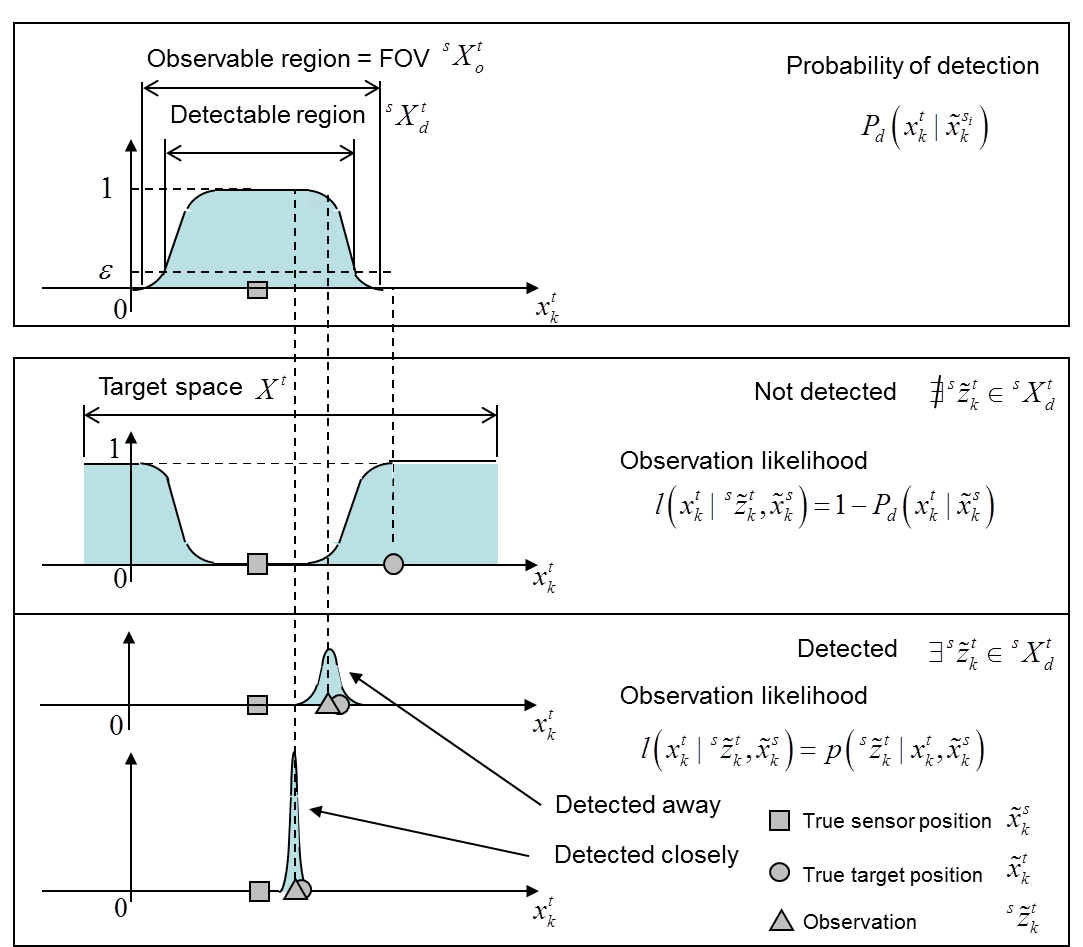
\includegraphics[width = \columnwidth]{optical.png} % PDF
	\caption{Optical observation likelihood}
	\label{fig:optical}
\end{figure}


%%%%%%%%%%%%%%%%%%%%%%%%%%%%%%%%%%%%%%%%
% Subsection
\subsection{Grid-based Method}
\label{sec:gmethod}
Handling the heavily non-Gaussian no-detection likelihood necessitates the grid-based method for RBE.  As the grid-based method represents the belief space in terms of regularly aligned grid cells, let the cell of concern be positioned at $l$th and $m$th partitions in $x$ and $y$ directions.  At the grid cell $\bl{l,m}$, the prediction and the correction are processed independently.  The prediction requires the numerical evaluation of the Chapman-Kolmogorov equation in Equation (\ref{eq:predictT}) at each grid cell. Given the belief $p_{\Vxbp{k-1}{t}}^{l,m}\bs{\ptVzbp{s}{1:k-1}{t}}$ at time step $k$ as well as the motion model $p_{\Vxbp{k}{t}|\Vxbp{k-1}{t}}^{l,m}$ constructed in the matrix form as the convolution kernel, the target belief at the grid cell $\bl{l,m}$ can be predicted as
\begin{eqnarray}\label{eq:predictTGM}
p_{\Vxbp{k}{t}}^{l,m}\bs{\ptVzbp{s}{1:k-1}{t}} = \sum_{\alpha=0}^{I_x^{t}} \sum_{\beta=0}^{I_y^{t}} p_{\Vxbp{k}{t}|\Vxbp{k-1}{t}}^{\alpha,\beta} p_{\Vxbp{k-1}{t}}^{l-\alpha,m-\beta}\bs{\ptVzbp{s}{1:k-1}{t}}.
\end{eqnarray}
where $\otimes$ indicates the convolution of the last belief with the motion model.  

The correction requires the computation of Equation (\ref{eq:correctT}) at each grid cell.  Given the predicted belief $p_{\Vxbp{k}{t}}^{l,m}\bs{\ptVzbp{s}{1:k-1}{t}}$ and the observation likelihood
$l_{\Vxbp{k}{t}}^{l,m}\bs{\ptVzbp{s}{k}{t}}$, the target belief at the grid cell $\bl{l,m}$ can be corrected as
\begin{eqnarray}\label{eq:correctTGM}
p_{\Vxbp{k}{t}}^{l,m}\bs{\ptVzbp{s}{1:k}{t}} = \frac{q_{\Vxbp{k}{t}}^{l,m}\bs{\cdot}}
{\Delta x_r \Delta y_r \sum_{\alpha} \sum_{\beta} q_{\Vxbp{k}{t}}^{\alpha,\beta}\bs{\cdot}},
\end{eqnarray}
where
\begin{eqnarray}\label{eq:correctTGM2}
q_{\Vxbp{k}{t}}^{l,m}\bs{\ptVzbp{s}{1:k}{t}} = l_{\Vxbp{k}{t}}^{l,m}\bs{\ptVzbp{s}{k}{t}} p_{\Vxbp{k}{t}}^{l,m}\bs{\ptVzbp{s}{1:k-1}{t}}.
\end{eqnarray}
and $\bl{\Delta x_r, \Delta y_r}$ is the size of the grid.  

Whilst the generalized optical observation likelihood allows belief update and maintenance regardless of whether the target has been detected, the RBE with the optical observation likelihood does not update and maintain the belief effectively.  Figure~\ref{fig:FOV} illustratively depicts this problem where the FOV and the NFOV are given by the light blue and the white colors respectively.  When the configuration of the target space is constrained complicatedly, the FOV becomes significantly limited compared to the target space.  This makes the belief dominantly updated by the observation likelihood with no detection.  If no detection continuously takes place, the belief keeps spread out with predictions and becomes highly uncertain and unreliable.  The next section will describe the proposed target estimation incorporating an acoustic sensor to solve this problem.  

\begin{figure}[ht]
	\centering
	\includegraphics[width=0.6\columnwidth]{FOV.png} % PDF
%	\includegraphics[bb = 0 0 792 621, width=5cm]{Figures/FOV.png} %DVI
	\caption{Optical observation likelihood}
	\label{fig:FOV}
\end{figure}


%%%%%%%%%%%%%%%%%%%%%%%%%%%%%%%%%%%%%%%%%%%%%%%%%%%%%%%%%%%%%%%%%%%%%%%%%%%%%%%%
% SECTION
%%%%%%%%%%%%%%%%%%%%%%%%%%%%%%%%%%%%%%%%%%%%%%%%%%%%%%%%%%%%%%%%%%%%%%%%%%%%%%%%
\section{Target Estimation Incorporating Optical and Acoustic Sensors}
\label{sec:acoustic}
%%%%%%%%%%%%%%%%%%%%%%%%%%%%%%%%%%%%%%%%
% Subsection
\subsection{Acoustic Sensor Model and Observation Likelihood}
The acoustic sensor incorporated in the proposed approach can observe a target on the non-line-of-sight (NLOS) or even in the NFOV though accuracy is limited due to the complex behavior of sound signals including reflection, refraction and diffraction.  Because of its broad range, the observable region of the acoustic sensor could be considered unlimited when compared to that of the optical sensor.  The acoustic sensor model $s_a$ can be therefore constructed without defining an observable region unlike the optical sensor model: 
\begin{equation}\label{eq:acoustic_sensor_model}
\pVzbp{s_a}{k}{t} = \pVhp{s_a}{t}{\Vxbp{k}{t},\tVxbp{k}{s},\pVvbp{s_a}{k}{t}}, 
\end{equation}
which is probabilistically equivalent to the likelihood given by 
\begin{equation}\label{eq:acoustic_likelihood}
\lia{\Vxbp{k}{t}|\ptVzbp{s_a}{k}{t},\tVxbp{k}{s}} = \p{\ptVzbp{s_a}{k}{t}|\Vxbp{k}{t},\tVxbp{k}{s}}. 
\end{equation}

Figure \ref{fig:acoustic} illustrates the observation likelihood of the acoustic sensor in comparison to that of the optical sensor in Figure \ref{fig:optical}.  The observation likelihood could be heavily non-Gaussian with multiple peaks if the target is on the NLOS though it is highly likely that one of the peaks is found near the location of the target as shown in the figure.  The likelihood with a target on the LOS could still be multi-modal if there are adjacent structures that create reflective, refractive and/or diffractive sound signals, but it captures the target location more confidently with a sharper peak.  The likelihood with a target on the LOS without adjacent structures will be a sharp near-Gaussian distribution since the direct sound dominates the observation.  

\begin{figure}[ht]
	\centering
	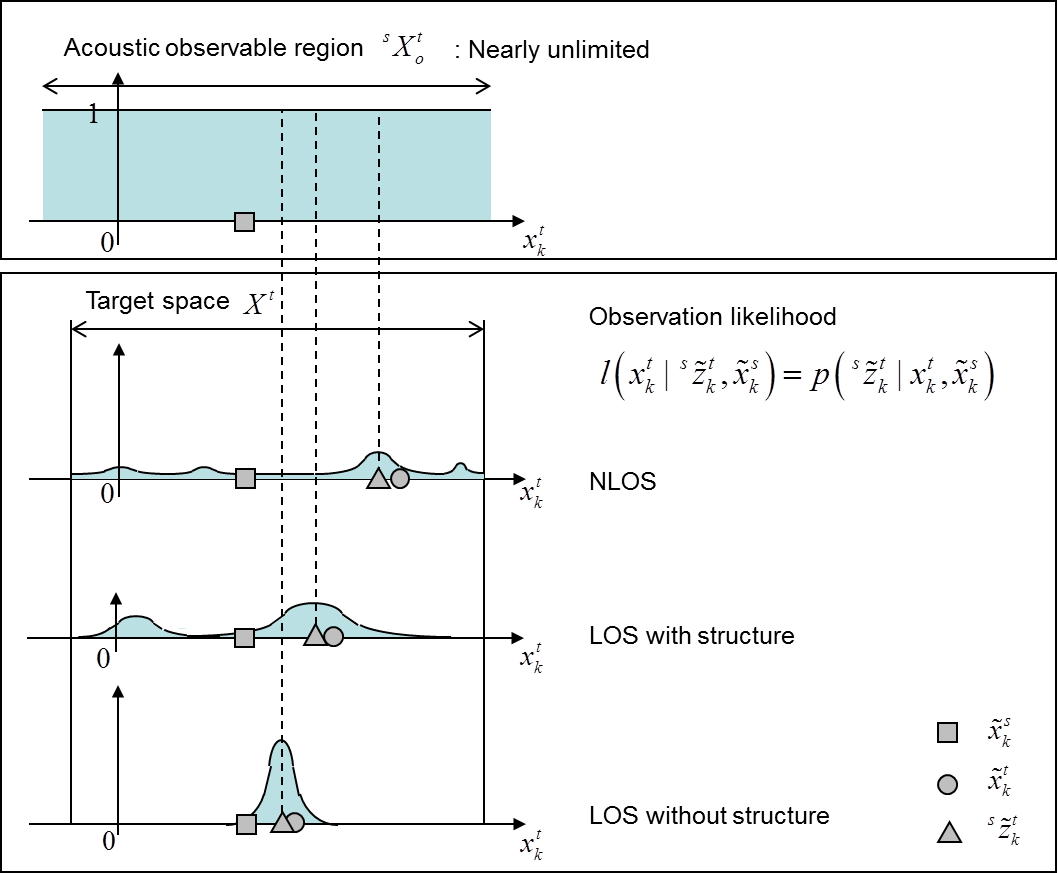
\includegraphics[width = \columnwidth]{acoustic.png} % PDF
	\caption{Acoustic observation likelihood}
	\label{fig:acoustic}
\end{figure}

%%%%%%%%%%%%%%%%%%%%%%%%%%%%%%%%%%%%%%%%
% Subsection
\subsection{RBE Using Joint Optical/Acoustic Observation Likelihood}
Given the observation likelihood of the optical sensor $\lio{\Vxbp{k}{t}|\ptVzbp{s}{k}{t},\tVxbp{k}{s}}$ and that of the acoustic sensor \linebreak[4] $\lia{\Vxbp{k}{t}|\ptVzbp{s}{k}{t},\tVxbp{k}{s}}$, the proposed approach derives a joint likelihood by multiplying the two likelihoods: 
\begin{equation}\label{eq:joint}
\li{\Vxbp{k}{t}|\ptVzbp{s}{k}{t},\tVxbp{k}{s}} = \lio{\Vxbp{k}{t}|\ptVzbp{s}{k}{t},\tVxbp{k}{s}} \lia{\Vxbp{k}{t}|\ptVzbp{s}{k}{t},\tVxbp{k}{s}} 
\end{equation}
in accordance to the canonical data fusion formula.  The joint optical/acoustic likelihood may not be a probability density similarly to the optical and acoustic observation likelihoods. 

Figure \ref{fig:joint} illustratively shows the resulting joint optical/acoustic observation likelihood when the target is in the NFOV.  The possible locations of the target are narrowed down since the optical likelihood with no detection clears out likelihood in the detectable region and dropped some peak(s) as shown in the figure.  However, the joint likelihood could still remain heavily non-Gaussian with multiple peaks and thus may not solely make a good estimation about where the target is.  


\begin{figure}[ht]
	\centering
	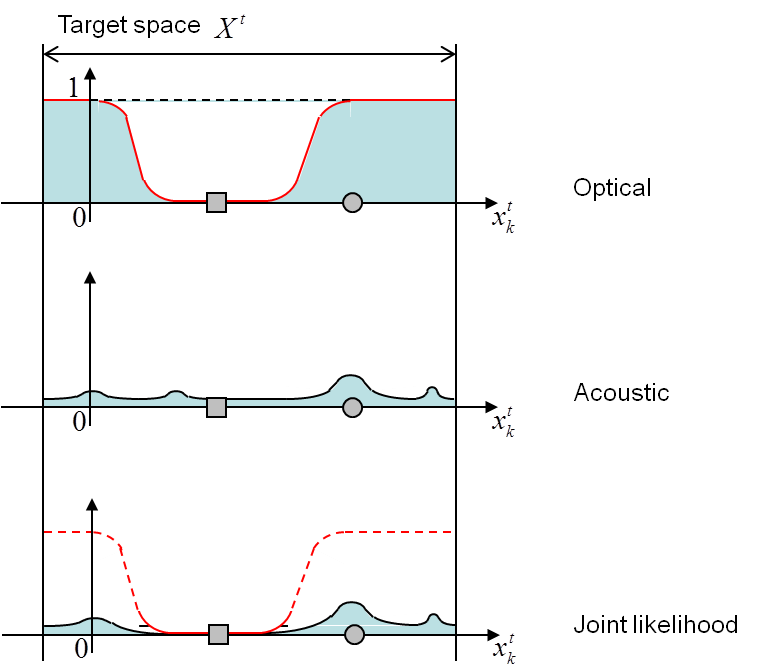
\includegraphics[width=0.8\columnwidth]{joint.png} % PDF
	\caption{Joint optical/acoustic observation likelihood}
	\label{fig:joint}
\end{figure}

Figure \ref{fig:jointRBE} shows the further ability of the proposed approach in reliable target estimation.  The proposed approach performs RBE by using the joint likelihood in correction (substituting Equation (\ref{eq:joint}) into Equation (\ref{eq:qT})) within the standard RBE framework.  Because sharpest and most Gaussian is the optical observation likelihood with detection, the prior belief is most determined by the last optical observation and remains a sharp Gaussian distribution.  The posterior belief with the joint observation likelihood inherits this characteristics since the joint likelihood most likely captures the target location with a peak and magnifies the confidence of the prior belief with the joint likelihood.  


\begin{figure}[ht]
	\centering
	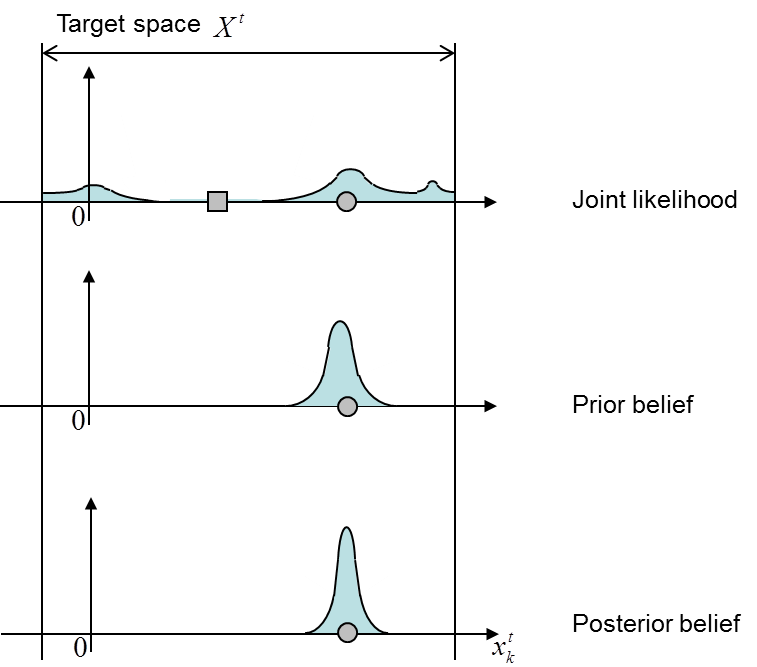
\includegraphics[width=0.8\columnwidth]{posterior.png} % PDF
	\caption{RBE incorporating an acoustic sensor}
	\label{fig:jointRBE}
\end{figure}


%%%%%%%%%%%%%%%%%%%%%%%%%%%%%%%%%%%%%%%%
% Subsection
\subsection{Modeling of Acoustic Observation Likelihood}
The technique proposed in this paper to model an acoustic observation likelihood uses two microphones as an acoustic sensor and constructs acoustic cues of the target in the environment of concern \textit{a priori}.  This is because of the potential of the proposed technique for NLOS target estimation through the preliminary investigations of the authors \cite{kim12,kum11,nod12} and inability of the aforementioned existing techniques.  Figure~\ref{fig:acoustic sensor} shows a schematic diagram of the proposed technique to model an acoustic observation likelihood.  We assume that the target emits sound with white noise, and we indeed use it to create the acoustic observation likelihood.  A white noise sound emitted at a specific position by the target for a certain time period is first recorded by two microphones.  After applying fast Fourier transform (FFT), the difference between the frequency-domain amplitude responses, known as the ILD, is then derived and further sampled to form an ILD vector within the frequency range of interest.  The ILD vector is created with various target positions and each saved as an acoustic cue.  The acoustic observation likelihood modeling essentially corresponds to creating the set of ILD vectors.  When a target emitted a white noise sound, the ILD vector of the sound observation is compared to all the acoustic cues.  The degree of similarity is then used to develop a correlation map indicating where the target is likely to be.  The correlation map is the acoustic likelihood of the particular sound observation.  


\begin{figure}[ht]
	\centering
	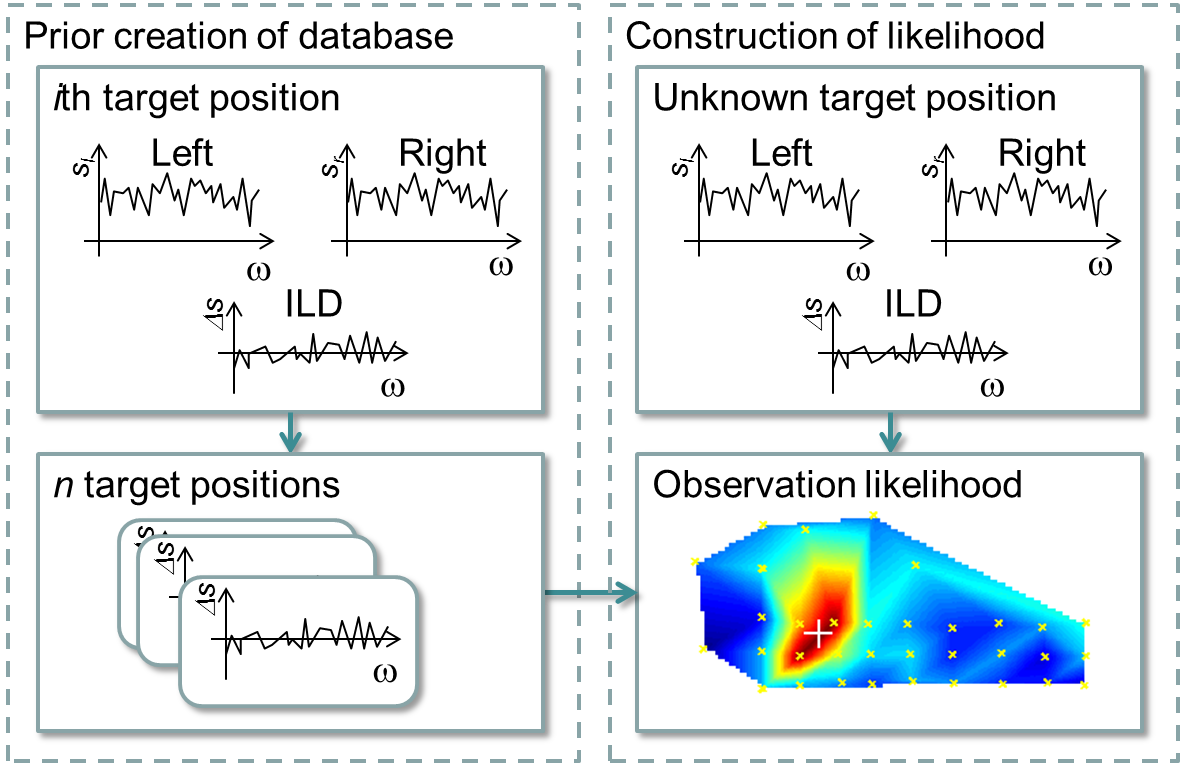
\includegraphics[width = 8cm]{likelihood.png} % PDF
	\caption{Acoustic sensor}
	\label{fig:acoustic sensor}
\end{figure}

Mathematically, let the frequency-domain sound \linebreak[4]level of the target at the $i$th position $\bs{\Vxbp{k}{t}}_{i}$, which is observed by the left and right microphones, be $s_l\bs{\omega|\bs{\Vxbp{k}{t}}_{i}}$ and $s_r\bs{\omega|\bs{\Vxbp{k}{t}}_{i}}$ where $\omega$ is a frequency of sound.  The ILD for the $i$th position $\bs{\Vxbp{k}{t}}_{i}$, $\Delta S\bs{\omega|\bs{\Vxbp{k}{t}}_i}$, is then given by 
\begin{eqnarray}\label{eq:ILD}
\lefteqn{\Delta S\bs{\omega|\bs{\Vxbp{k}{t}}_i}} \nonumber\\  &&= 20 \log \abs{s_l\bs{\omega|\bs{\Vxbp{k}{t}}_{i}}} - 20 \log \abs{s_r\bs{\omega|\bs{\Vxbp{k}{t}}_{i}}}.  
\end{eqnarray}
If the ILD is sampled at $N$ frequencies {\small{$\V{\Omega} = \bl{\omega_1,\ldots,\omega_N}^\top$}}, the ILD vector can be described as 
\begin{eqnarray}\label{eq:ILDs}
\lefteqn{\V{S}\bs{\V{\Omega}|\bs{\Vxbp{k}{t}}_i}}\nonumber\\ &&= \bl{a_1 \Delta S\bs{\omega_1|\bs{\Vxbp{k}{t}}_i},\ldots, a_N \Delta S\bs{\omega_N|\bs{\Vxbp{k}{t}}_i}}^\top,
\end{eqnarray}
where 
\begin{equation}
a_{j} = \mac{\min\bm{\abs{s_l\bs{\omega_j|\bs{\Vxbp{k}{t}}_{i}}},\abs{s_r\bs{\omega_j|\bs{\Vxbp{k}{t}}_{i}}}}-\epsilon}. 
\end{equation}
In the equation, $\mac{\cdot}$ is Macaulay brackets, and $\min\bm{\cdot,\cdot}$ returns the smaller value of the two entities. \thl{Thus, $a_j$ effectively filters noise components of the signal.} When the ILD vector is created with a set of frequencies $\tV{\Omega}$ at $n$ known target positions, i.e., $\bs{\tVxbp{k}{t}}_i, \forall i \in \bm{1,...,n}$, the acoustic cues to be prepared in advance and used to create the acoustic observation likelihood become $\V{S}\bs{\tV{\Omega}|\bs{\tVxbp{k}{t}}_i}, \forall i \in \bm{1,...,n}$.  

Given the ILD vector $\V{S}\bs{\tV{\Omega}|\ptVzbp{s}{k}{t}}$ with observation $\ptVzbp{s}{k}{t}$ at unknown target position $\Vxbp{k}{t}$, the proposed technique quantifies the degree of correlation of the $i$th ILD vector to that of the unknown target position as
\begin{eqnarray}\label{eq:correlation}
\lefteqn{X\bs{\bs{\tVxbp{k}{t}}_i | \ptVzbp{s}{k}{t}}} \nonumber \\ &&= \frac{1}{2} \bm{\frac{\V{S}\bs{\tV{\Omega}|\ptVzbp{s}{k}{t}}^\top \V{S}\bs{\tV{\Omega}|\bs{\tVxbp{k}{t}}_i}}{\abs{\V{S}\bs{\tV{\Omega}|\ptVzbp{s}{k}{t}}}\abs{\V{S}\bs{\tV{\Omega}|\bs{\tVxbp{k}{t}}_i}}}-1}. 
\end{eqnarray}
where $0 \leq X\bs{\cdot} \leq 1$.  The acoustic observation likelihood with the unknown target position $\Vxbp{k}{t}$ can be finally calculated as
\begin{eqnarray}\label{eq:acoustic}
\lia{\Vxbp{k}{t}|\ptVzbp{s}{k}{t},\tVxbp{k}{s}} = \sum_{i=1}^n{\mu_{i}\bs{\boldsymbol{\xi}_k^t} X\bs{\bs{\tVxbp{k}{t}}_i | \ptVzbp{s}{k}{t}}},
\end{eqnarray}
where $\mu_{i}\bs{\boldsymbol{\xi}_k^t}$ is a basis function of natural coordinates $\boldsymbol{\xi}_k^t$, which are transformed from $\Vxbp{k}{t}$. Based on the characteristics of the likelihood, the proposed technique uses the T-spline basis function such that $\mu_{i}\bs{\boldsymbol{\xi}_k^t}$ in a T-mesh, for the two-dimensional parameter space case $\boldsymbol{\xi}_k^t = \bl{\xi_k^t,\eta_k^t}^\top$, can be represented as
\begin{eqnarray}
\mu_{i}\bs{\boldsymbol{\xi}_k^t} = \mu_{i}^1 \bs{\xi_k^t} \mu_{i}^2 \bs{\eta_k^t}
\end{eqnarray}
where $\mu_{i}^{\bs{\cdot}}$ is a cubic B-spline basis function. Further detailed formulations are found in \cite{sederberg2003}.  It is to be noted here that other basis functions are also possible while the proposed technique uses T-spline basis functions. 


%%%%%%%%%%%%%%%%%%%%%%%%%%%%%%%%%%%%%%%%%%%%%%%%%%%%%%%%%%%%%%%%%%%%%%%%%%%%%%%%
% SECTION
%%%%%%%%%%%%%%%%%%%%%%%%%%%%%%%%%%%%%%%%%%%%%%%%%%%%%%%%%%%%%%%%%%%%%%%%%%%%%%%%
\section{NUMERICAL AND EXPERIMENTAL ANALYSIS}
\label{sec:examples}
The efficacy of the proposed approach was examined experimentally in two steps.  The first step was aimed at studying the capability and limitation of the proposed acoustic sensing technique by parametrically changing the complexity of the environment where the experimental system with a speaker array and a movable/replaceable wall was developed specifically for this study.  After verifying the feasibility of the acoustic sensing for NLOS target localization, the applicability of the proposed approach to the estimation of a NFOV target in a complex practical environment was investigated.  The investigation looked into the performance of both the joint optical/acoustic observation likelihood and the RBE with the joint likelihood.  


\subsection{Acoustic Observation of NLOS Target}
Figure~\ref{fig:pma} shows the design of the experimental system that changes the complexity of the environment for the evaluation of the proposed acoustic sensing technique.  An acoustic sensor consisting of two microphones is fixed next to an outer wall and faces open space where a speaker array and movable/replaceable wall(s) are placed.  The complexity of the environment can be changed by varying the two parameters of the movable/replaceable wall: the distance of the wall to the edge of speaker array $L_d$ and the length of the wall $L_w$.  The longer the distance and/or the larger the length, the more complex the environment since sound from speakers result in more reflections.  

Shown in the figure as blue crosses are speaker locations.  A microcontroller controls speakers so that each speaker sequentially emits white noise sound for a programmed period.  A set of ILDs for a wall setting can be thus collected automatically.  Once the ILDs are collected, the ability of the proposed acoustic sensing technique is evaluated by emitting sound from a speaker at some location within the area of the speaker array and identifying the location in the form of observation likelihood.  The location is not where one of the speakers of the speaker array is located to demonstrate the ability of the proposed technique in identifying the target at an arbitrary position.  

Figure~\ref{fig:pmb} shows the developed experimental system \linebreak[4]whereas the dimensions and other parameters used in the experiments are listed in Table~\ref{tab:s-noise}.  Sound was sampled and represented at 8,192 frequency bins within the audible range to capture its behavior accurately.  54 speakers were aligned to cover the open space.  The distance and the length of the wall were varied to introduce both lightly NLOS and heavily NLOS environments.  The case of two walls ($n_w=2)$ were tested in addition to the single wall case to make the environment more complex.  The distance of only the wall closer to the acoustic sensor was varied.  


\begin{figure}[ht]
	\centering
  \subfigure[Schematic design]{
    \label{fig:pma}
    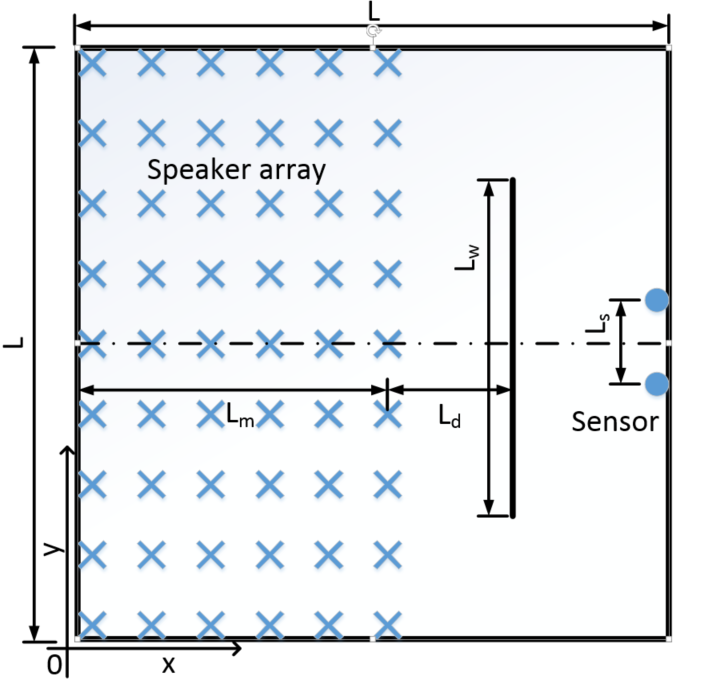
\includegraphics[width=0.46\columnwidth]{experiment_schematics3.png} % PDF
}
  \subfigure[Developed system]{
    \label{fig:pmb}
    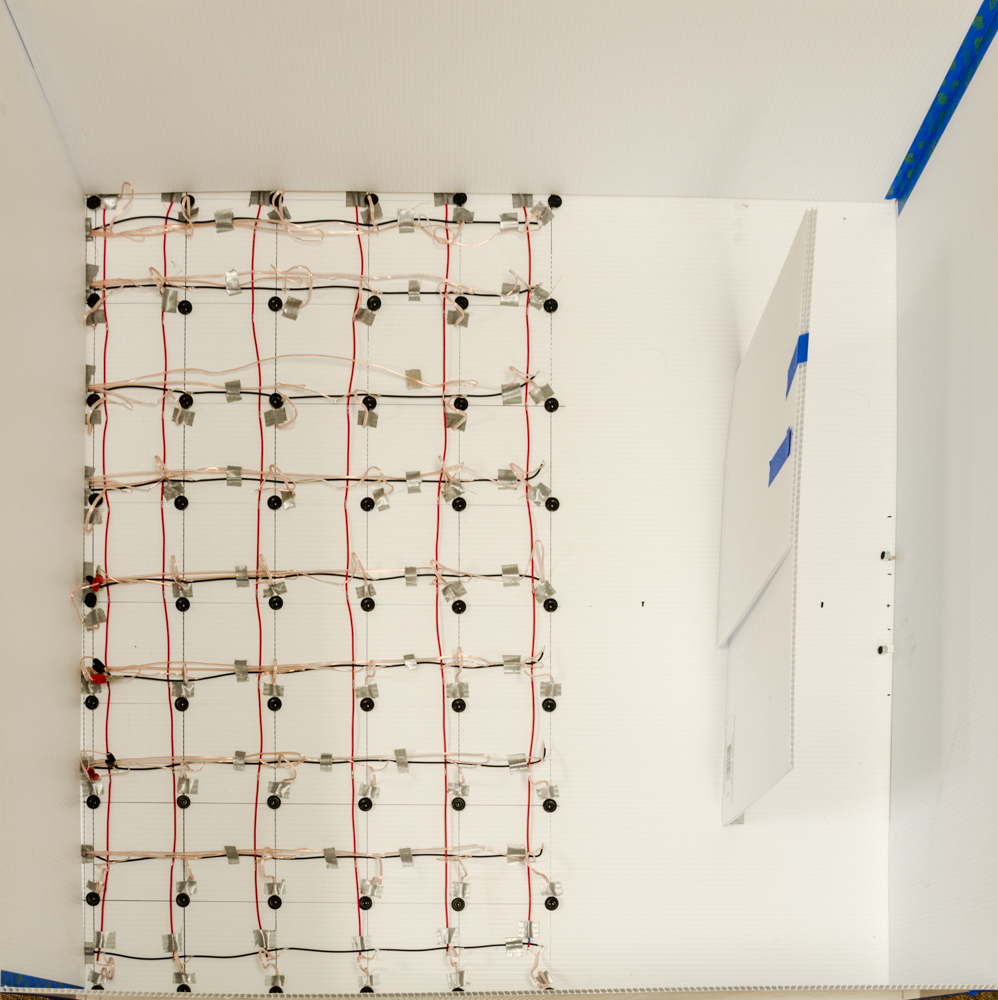
\includegraphics[width=0.46\columnwidth]{experiment_photo.jpg} % PDF
  }
	\caption{Experimental system for investigating influence of environmental complexity}
	\label{fig:p-map}
\end{figure}

\begin{table}[htbp]
\centering \caption{Dimensions and other parameters in the experiments}
\label{tab:s-noise}
\begin{tabular}{r|r||r|r}
\hline\noalign{\smallskip}
\footnotesize{Parameter} & Value & \footnotesize{Parameter} & Value\\
\noalign{\smallskip}\hline\noalign{\smallskip}
$\tVxp{t}$ & $\bl{42, 34}$ cm & $L$ &  90 cm \\
$\omega_1$ & 0 Hz & $L_{m}$ &  50 cm\\
$\omega_N$ & 22 kHz & $L_{s}$ &  10 cm\\
$N$ & 8,192 & $L_{d}$ &  $\bm{0,10,20,30}$ cm\\ 
$\epsilon$ & 0.01 & $L_{w}$ &  $\bm{50,60,70}$ cm\\
$n$ & 54 & $n_{w}$ & $\bm{1,2}$\\
\noalign{\smallskip}\hline\noalign{\smallskip}
\end{tabular}
\end{table}

\thl{Figure~{\ref{fig:ILDs}} shows the four ILDs each observed with a target at one of the 54 positions when $\bl{L_d, L_w, n_w} = \bl{50, 40, 1}$.  Two positions are on the LOS, and four are on the NLOS.  It is first seen that the configuration of the ILD varies depending on the target position.  The configuration is different even when the target is on the NLOS.  This indicates that the ILD contains information on the target position no matter whether the target is on the LOS. } 

\begin{figure}[ht]
	\centering
	\subfigure[$\bl{60,0}$ (LOS)]{
		\label{fig:l1}
		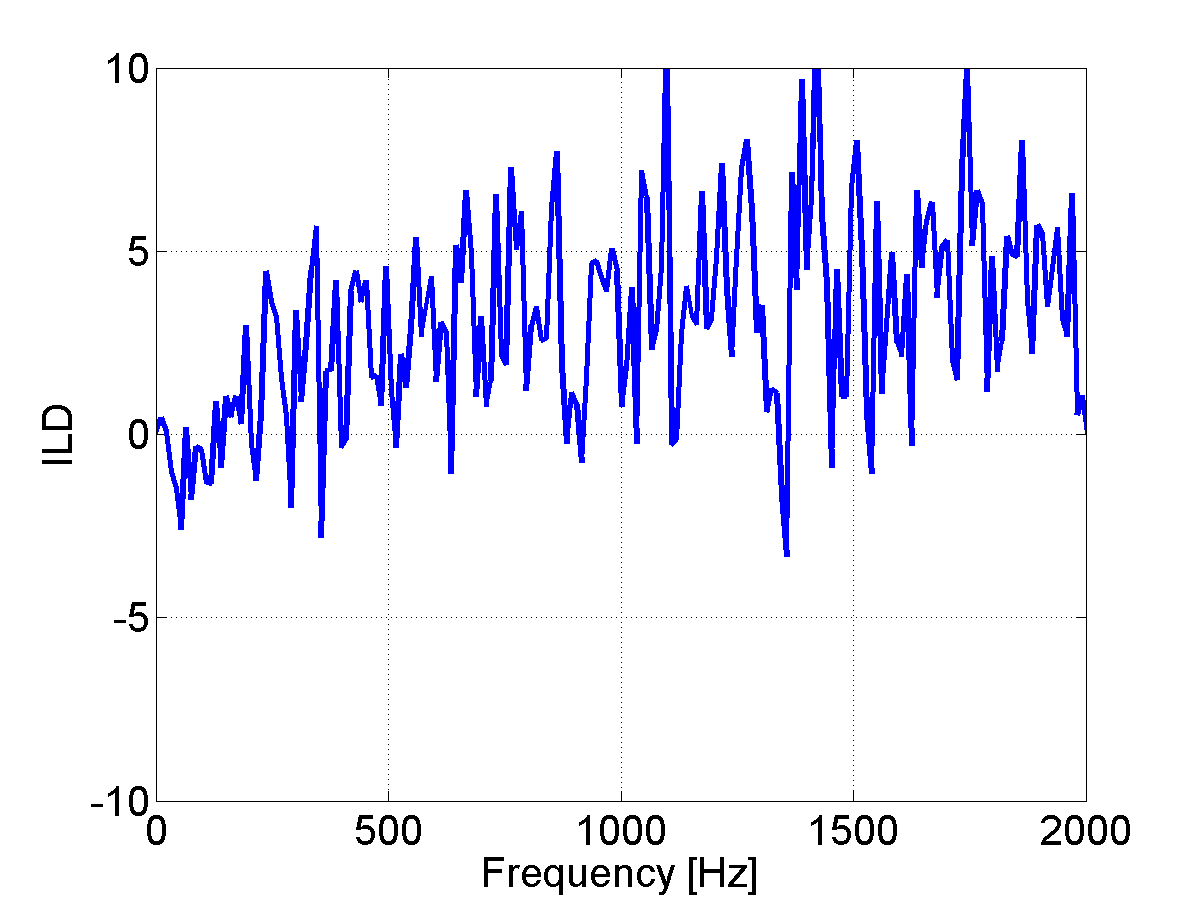
\includegraphics[width = 0.45\columnwidth]{step006.png} % PDF
		}
	\subfigure[$\bl{36,34}$ (NLOS)]{
		\label{fig:l2}
		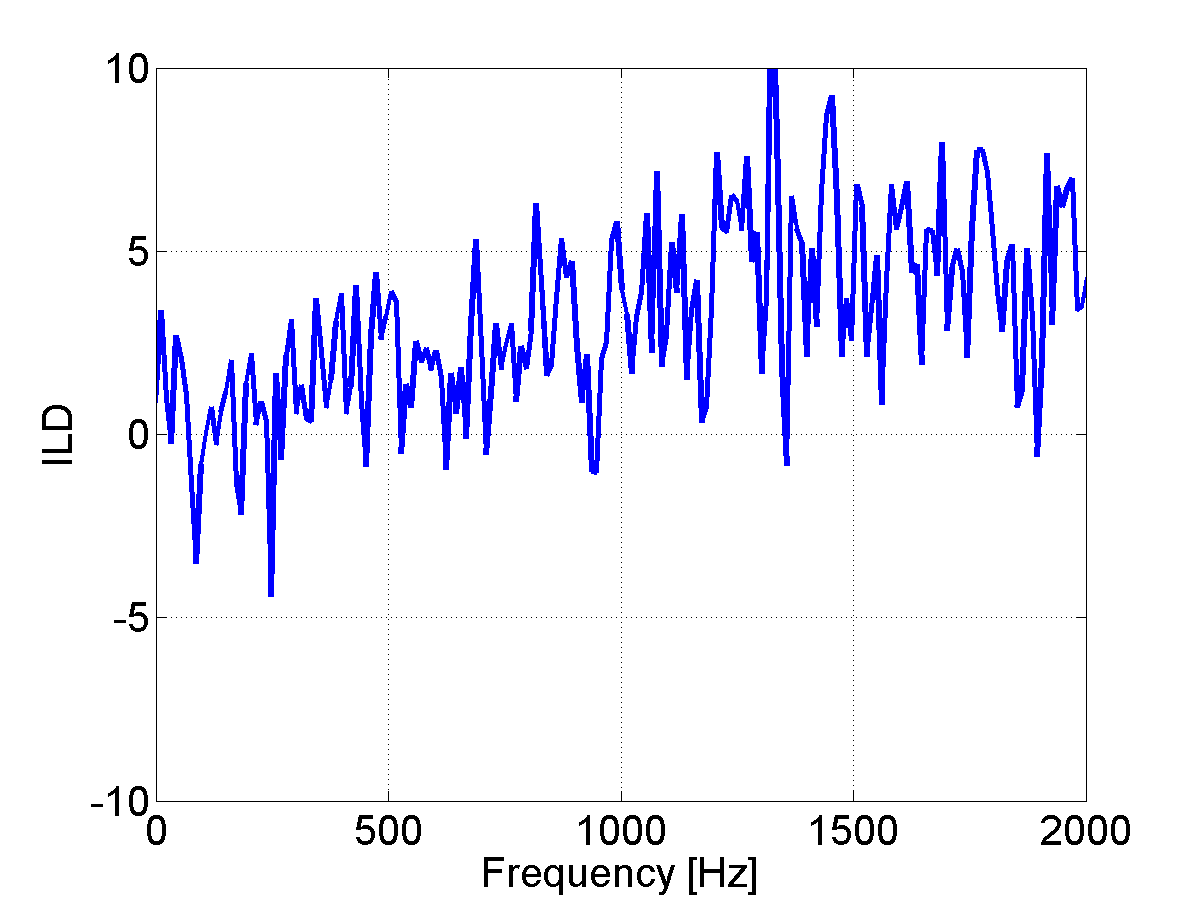
\includegraphics[width =  0.45\columnwidth]{step022.png} % PDF
	}
	\subfigure[$\bl{24,56}$ (NLOS)]{
		\label{fig:l3}
		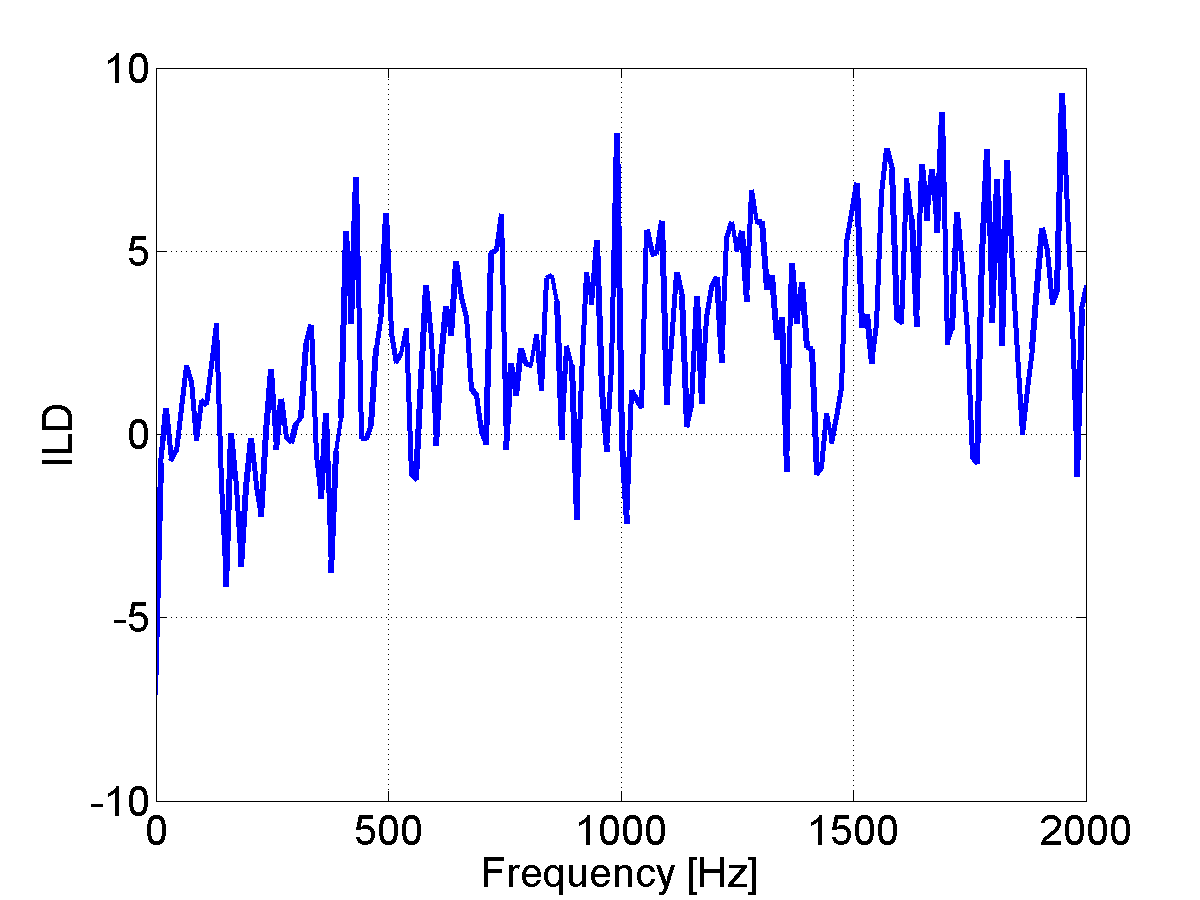
\includegraphics[width =  0.45\columnwidth]{step033.png} % PDF
	}
	\subfigure[$\bl{12,90}$ (LOS)]{
		\label{fig:l4}
		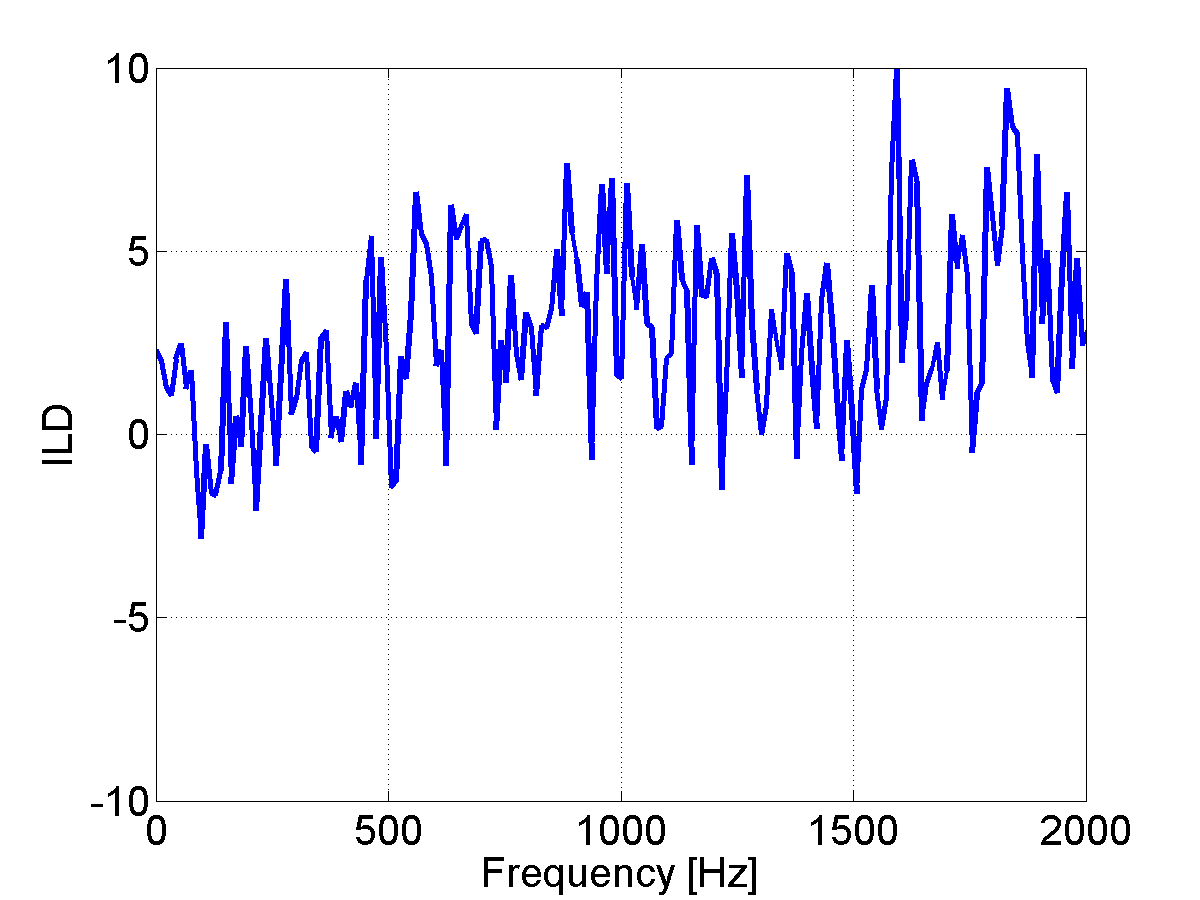
\includegraphics[width =  0.45\columnwidth]{step050.png} % PDF
	}
	\caption{ILDs at four of the 54 positions}
	\label{fig:ILDs}
\end{figure}

	
Figure~\ref{fig:EC-AL} shows four resulting acoustic observation likelihoods each with a different condition.  The former two cases are with a single wall having different distances and the same length whereas the latter two cases are with two walls having different lengths and the same distance.  The result first indicates that the target location is well estimated when the distance is short (Figure~\ref{fig:al1}) or when the length is small (Figure~\ref{fig:al3}).  The target is closer to LOS in these conditions since sound reaches the acoustic sensor with a small number of reflections.  The identification of the target location in the remaining two cases (Figures~\ref{fig:al2} and \ref{fig:al4}) is hard due to a number of sound reflections.  The identification with two walls (Figures~\ref{fig:al3} and \ref{fig:al4}) is seen to be harder than that with a single wall (Figures~\ref{fig:al1} and \ref{fig:al2}) for the same reason.  While the acoustic observation likelihood is heavily multi-modal in these cases, the target location is still captured by the highest peak (Figures~\ref{fig:al1}-\ref{fig:al3}) or at least by one of the peaks (Figure~\ref{fig:al4}).  This demonstrates the ability of the proposed acoustic sensing technique for identifying the location of the NFOV target though with limited accuracy.  
\begin{figure}[ht]
	\centering
  \subfigure[$L_d=0, L_w=70, n_w=1$]{
    \label{fig:al1}
    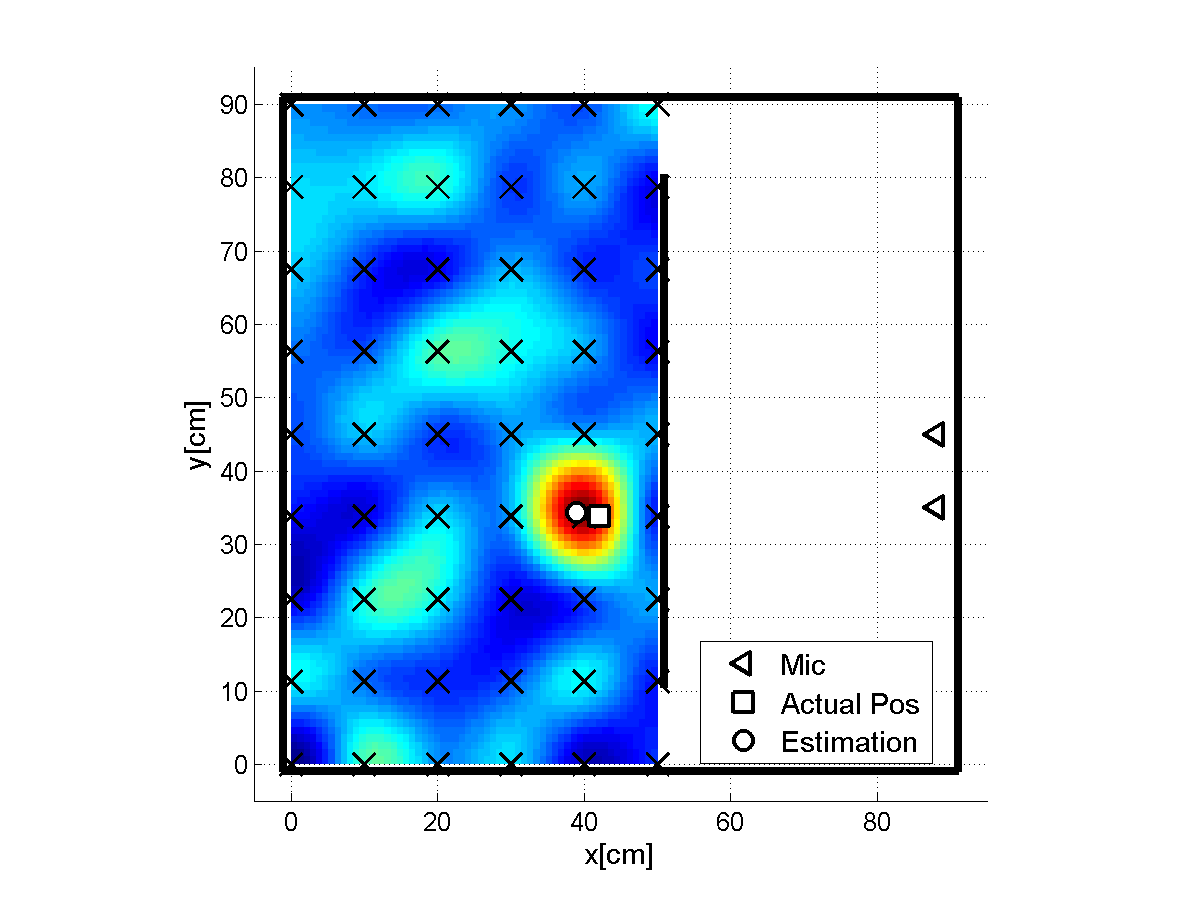
\includegraphics[trim = 30mm 5mm 30mm 15mm,clip,width = 0.468\columnwidth]{w1_Lw70_Ld0_step023.png} % PDF
  }
  \subfigure[$L_d=30, L_w=70, n_w=1$]{
    \label{fig:al2}
    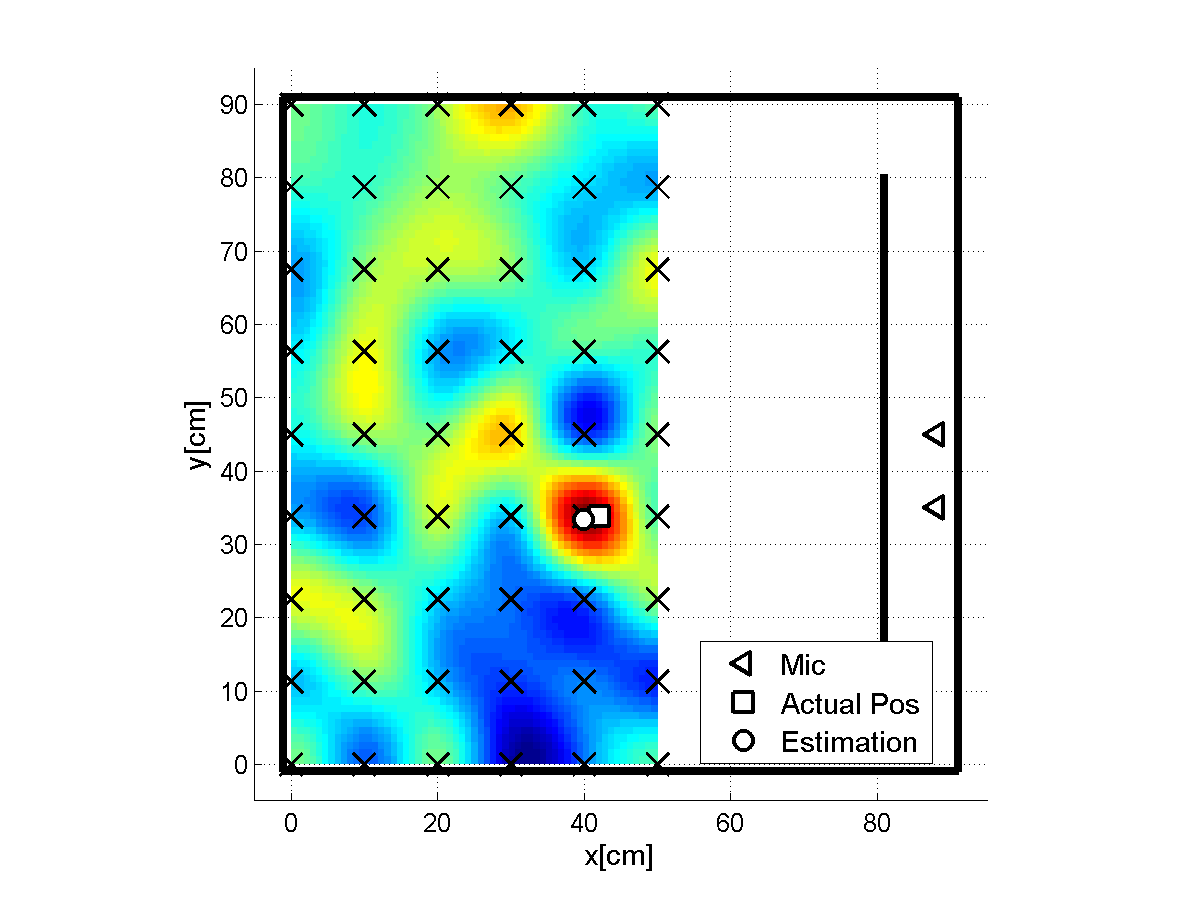
\includegraphics[trim = 30mm 5mm 30mm 15mm,clip,width =  0.468\columnwidth]{w1_Lw70_Ld30_step023.png} % PDF
  }
  \subfigure[$L_d=20, L_w=50, n_w=2$]{
    \label{fig:al3}
    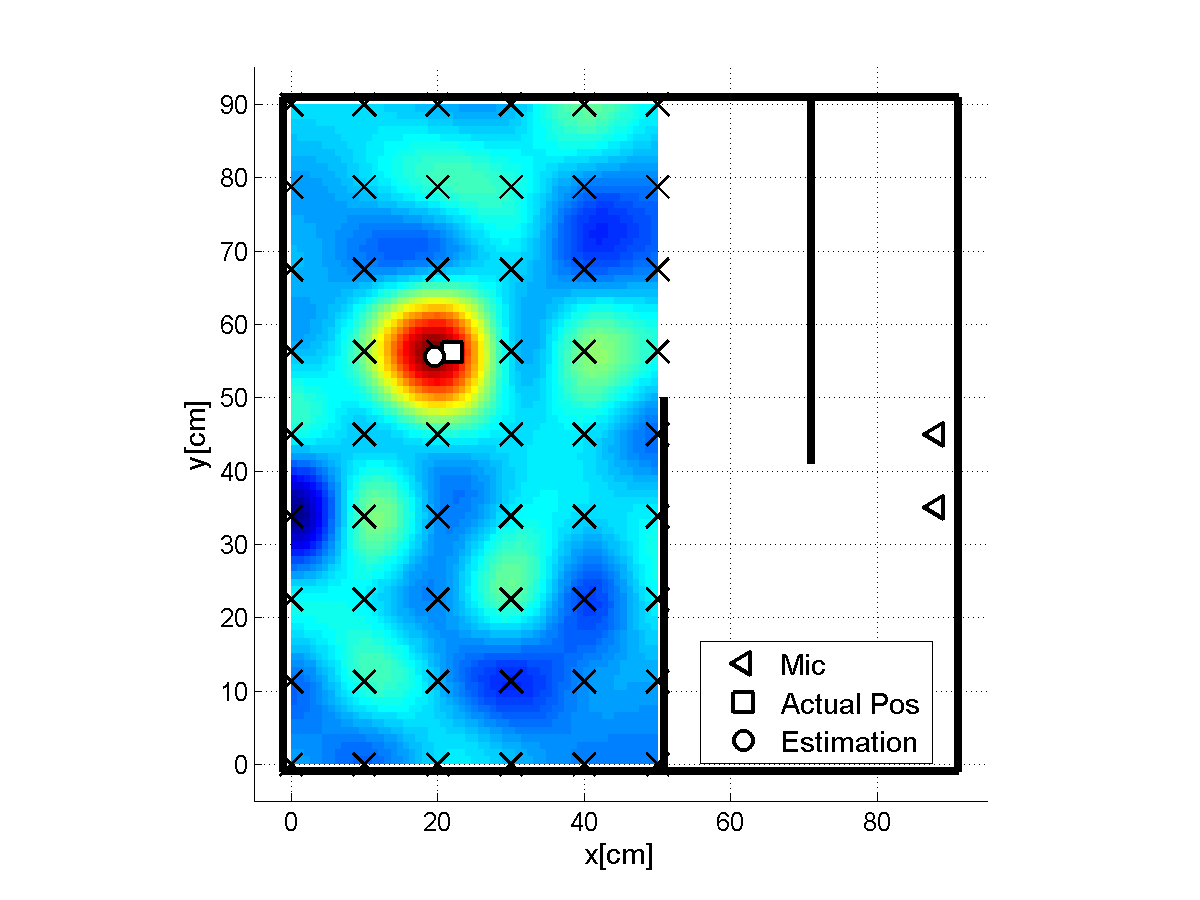
\includegraphics[trim = 30mm 5mm 30mm 15mm,clip,width =  0.468\columnwidth]{w2_Lw50_Ld20_step033.png} % PDF
  }
  \subfigure[$L_d=20, L_w=70, n_w=2$]{
    \label{fig:al4}
    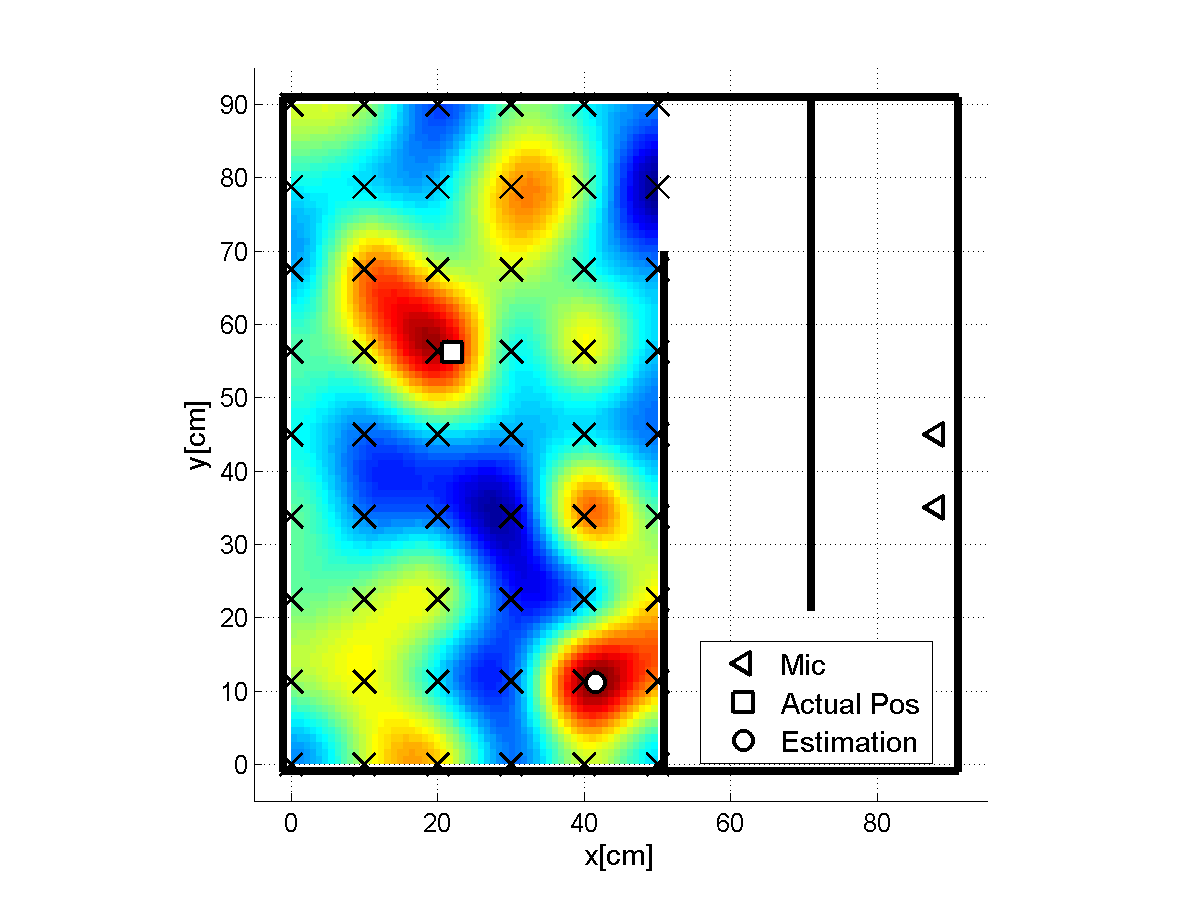
\includegraphics[trim = 30mm 5mm 30mm 15mm,clip,width =  0.468\columnwidth]{w2_Lw70_Ld20_step033.png} % PDF
}
	\caption{Acoustic observation likelihoods for different environmental complexity}
	\label{fig:EC-AL}
\end{figure}

Figure~\ref{fig:msw} and \ref{fig:mdw} show the mean error of the acoustic observation likelihood when the distance and the length were varied for single and double wall cases.  The mean error is a distance of the nearest peak of the acoustic observation likelihood to the true target location. The result of the mean error shows that the proposed technique could locate the target within $2$ cm error in most (11) of the 12 cases for single wall case.  The estimation is particularly good when the wall length was small.  The mean error with two walls, meanwhile, is over $20$ cm in four of nine cases.  This indicates that the proposed acoustic sensing technique is not sufficient enough for NLOS localization.  Figure~\ref{fig:de} shows the variation of the differential entropy with respect to the number of walls and the wall length.  It is seen that the addition of a wall dominantly increases uncertainty.  While the proposed acoustic sensing technique is effective enough in relatively simple NLOS environments, enhancement is necessary when target estimation in more complex environments is pursued.  

\begin{figure}[ht]
	\centering
  \subfigure[Single wall mean error]{
    \label{fig:msw}
    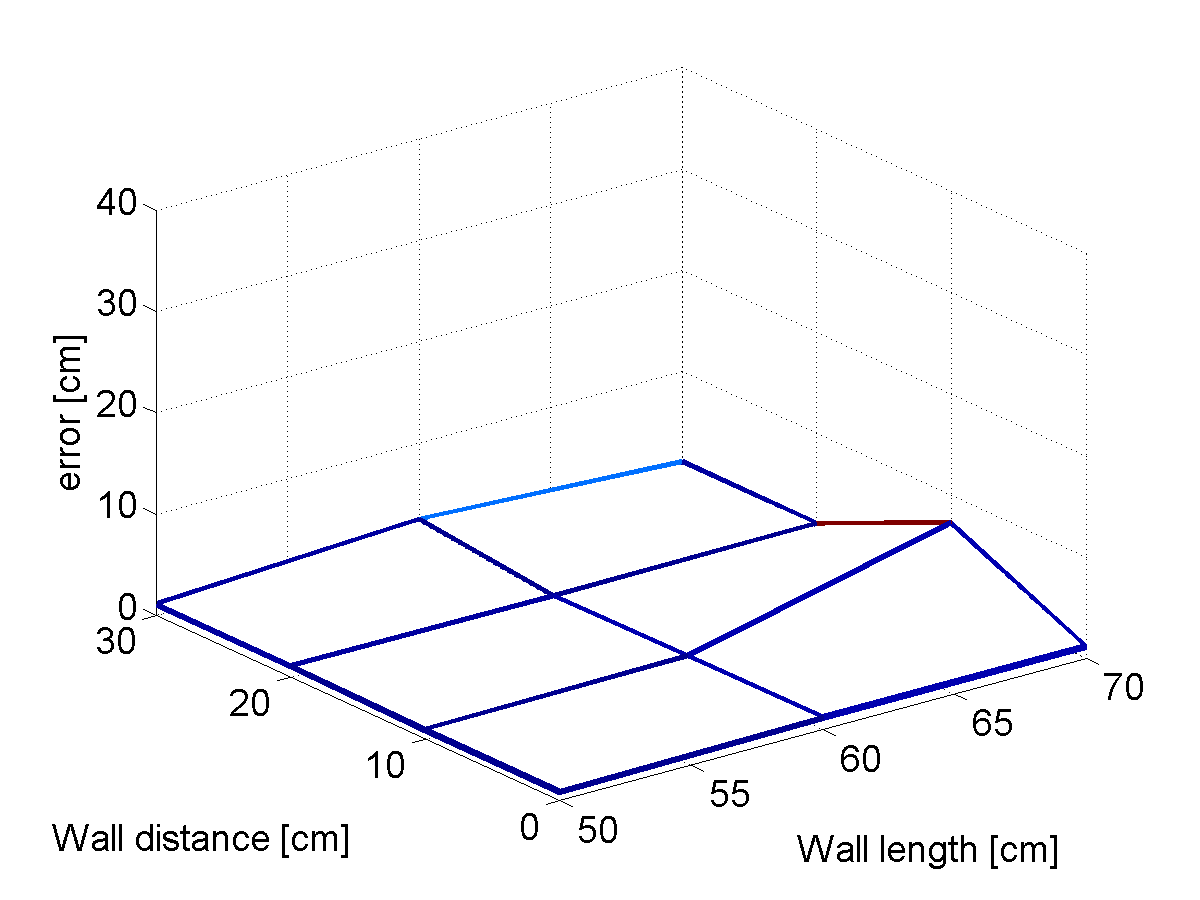
\includegraphics[width = 0.468\columnwidth]{w1_error.PNG} % PDF
  }
  \subfigure[Double wall mean error]{
    \label{fig:mdw}
	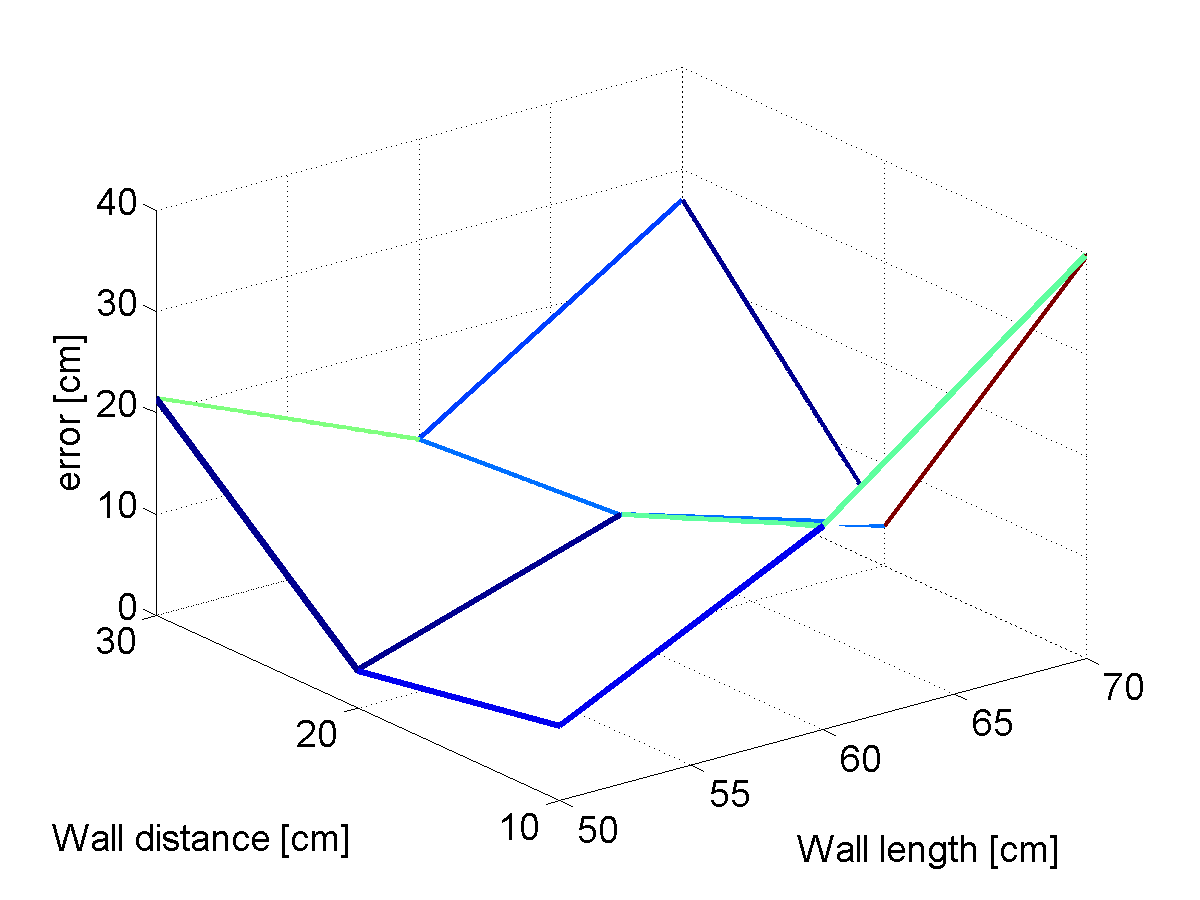
\includegraphics[width = 0.468\columnwidth]{w2_error.PNG}
  }
   \subfigure[Diferential entropy for single and double wall]{
   	\label{fig:de}
   	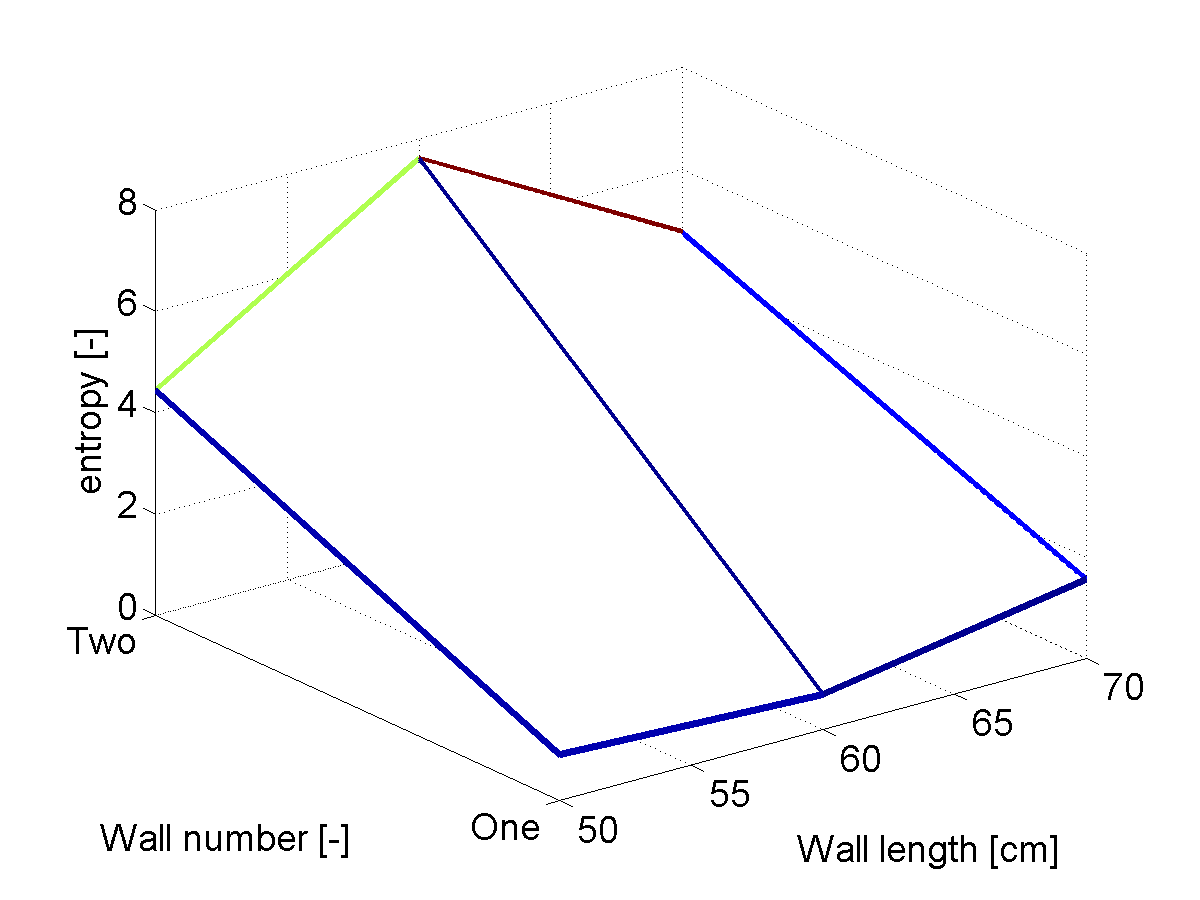
\includegraphics[width = 0.468\columnwidth]{H_1w2w.PNG} % PDF
  }
	\caption{Mean error and differential entropy of the acoustic observation likelihood with a single and double wall}
	\label{fig:EUSW}
\end{figure}

\subsection{NFOV Target Estimation in Complex Practical Environments}
This subsection investigates the applicability of the proposed approach to NFOV target estimation in complex practical environments by first enhancing the acoustic sensing with the optical sensing and then executing the RBE with the joint optical/acoustic observation likelihood.  Figure~\ref{fig:map} shows the map of the indoor environment used to demonstrate the practical applicability of the proposed approach as well as the details of the demonstration.  A sensor platform with a camera and two microphones for optical and acoustic observations was located in a corridor and faced with the open space the target could move around.  The environment is complex with the existence of walls and structures, so that the FOV of the camera is significantly limited compared to the target space.  Shown in the figure as yellow crosses are the target locations at which sound was emitted to collect ILDs.  After the collection, the target was then moved along the lines indicated in the figure and emitted sound.  The observation and estimation was examined at the four positions marked by red circles.  

Figure~\ref{fig:tsp} shows the target and the sensor platform.  The sensor platform is with a camera and two microphones as aforementioned whereas the target is a wireless speaker.  The same speaker was used to construct the acoustic observation likelihood.  White noise was emitted from the speaker, and the parameters used to construct the acoustic observation likelihood are listed in Table~\ref{tab:noise}.  

\begin{figure}[ht]
	\centering
	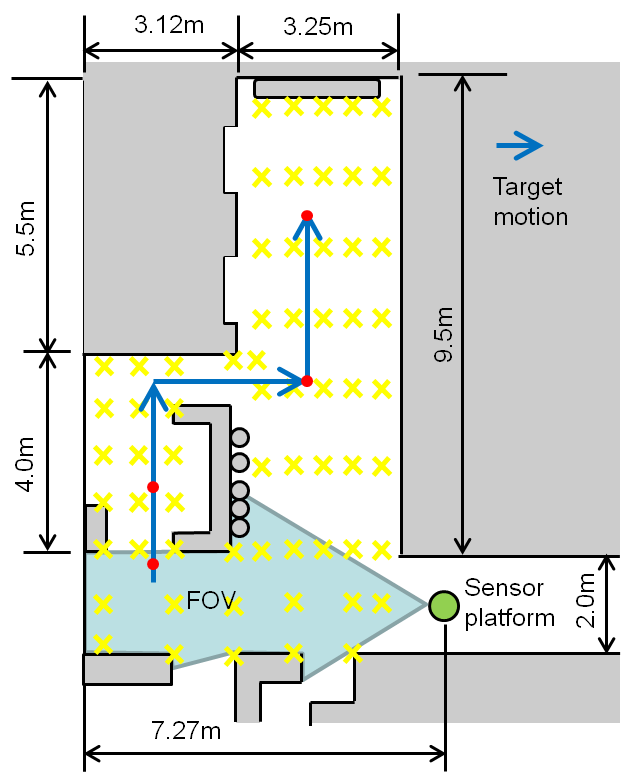
\includegraphics[width = 0.8\columnwidth]{map.png} % PDF
	\caption{Map of the test environment and demonstration}
	\label{fig:map}
\end{figure}

\begin{figure}[ht]
	\centering
	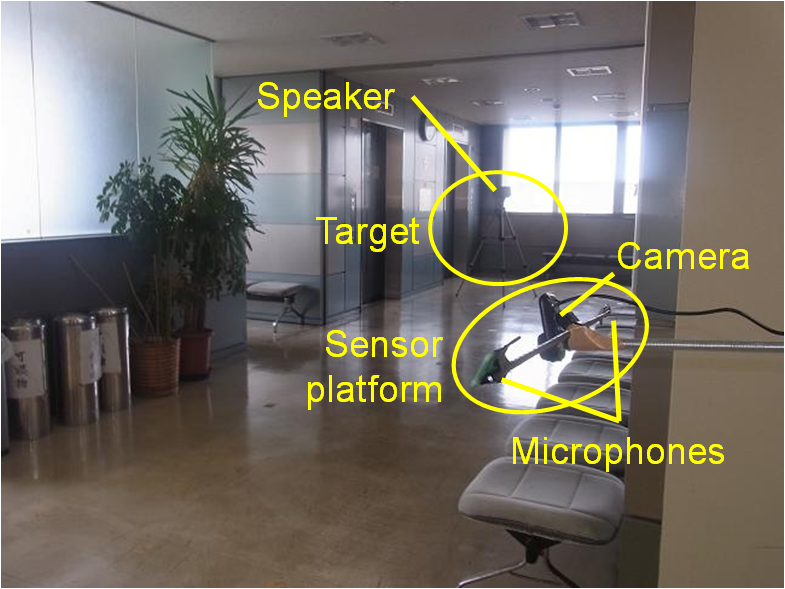
\includegraphics[width = 0.8\columnwidth]{system.png} % PDF
	\caption{Target and sensor platform}
	\label{fig:tsp}
\end{figure}

\begin{table}[htbp]
\centering \caption{Parameters for acoustic observation likelihood}
\label{tab:noise}
\begin{tabular}{r|r}
\hline\noalign{\smallskip}
Parameter & Value \\
\noalign{\smallskip}\hline\noalign{\smallskip}
$\omega_1$ & 0 [Hz]\\
$\omega_N$ & 386 [Hz] \\
$N$ & 100\\
$\epsilon$ & 0.01\\
$n$ & 65\\
\noalign{\smallskip}\hline\noalign{\smallskip}
\end{tabular}
\end{table}

%%%%%%%%%%%%%%%%%%%%%%%%%%%%%%%%%%%%%%%%
% Subsection
\subsubsection{Joint Optical/Acoustic Observation of NFOV Target}
Figure~\ref{fig:acoustic likelihoods} shows the acoustic observation likelihoods when the target moved and emitted sound at the four marked target positions, which are at the 1st, 7th, 35th and 51th steps.  The target is in the FOV only at the 1st step.  The acoustic observation likelihood is seen to be multi-modal due to sound reflection even when the target is within the FOV and thus on the LOS.  The proposed acoustic sensing technique has, however, been able to accurately identify the true target position at one of the peaks and successfully detect it except for the 7th step.  Failure in the 7th step is a result of the limitation of acoustic sensing shown and concluded in the last subsection, but it is to be importantly noted that the target position is captured near the second highest peak.  

\begin{figure}[ht]
	\centering
  \subfigure[$k=1$ (FOV)]{
    \label{fig:a1}
    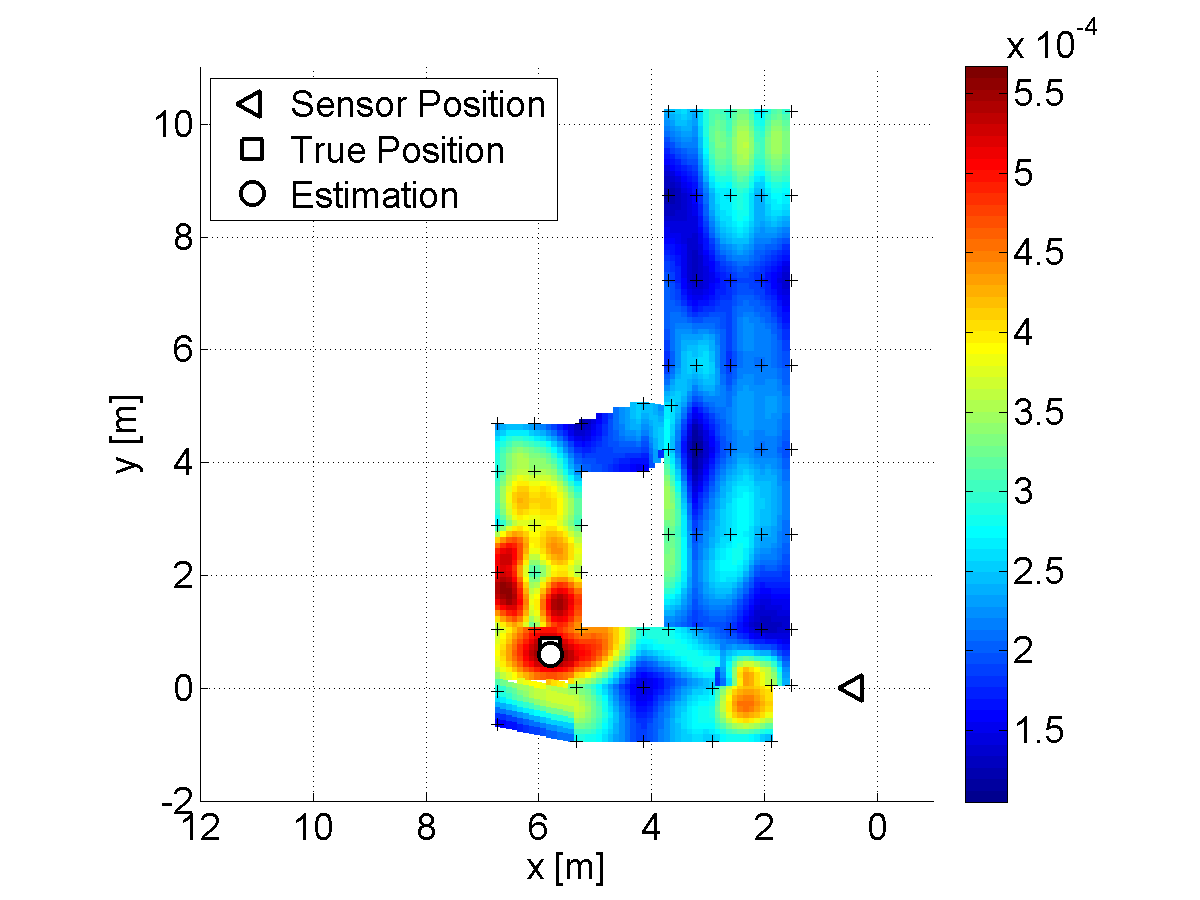
\includegraphics[trim = 15mm 0mm 15mm 0mm,clip,width = 0.46\columnwidth]{AOL_Figure1.png} % PDF
  }
  \subfigure[$k=7$ (NFOV)]{
    \label{fig:a2}
    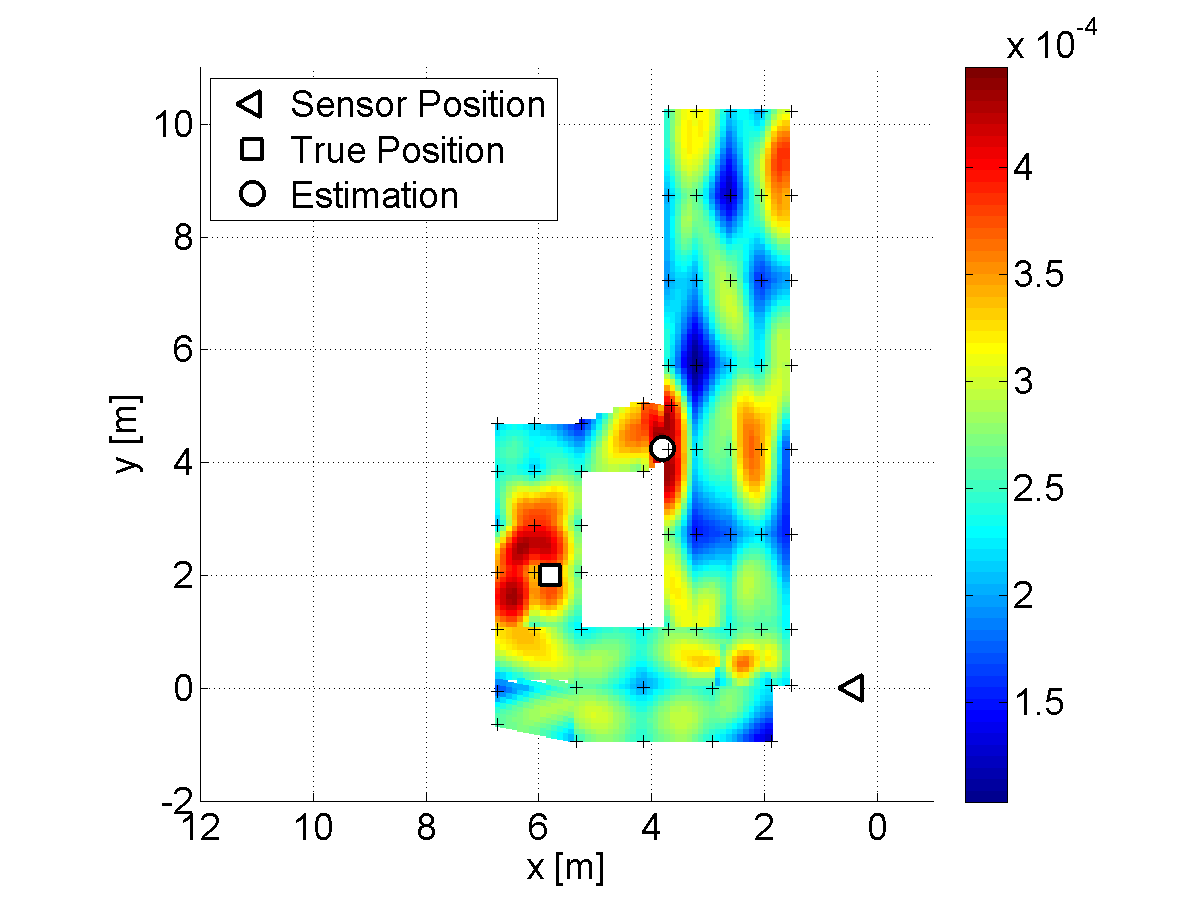
\includegraphics[trim =  15mm 0mm 15mm 0mm,clip,width = 0.46\columnwidth]{AOL_Figure2.png} % PDF
  }
  \subfigure[$k=35$ (NFOV)]{
    \label{fig:a3}
    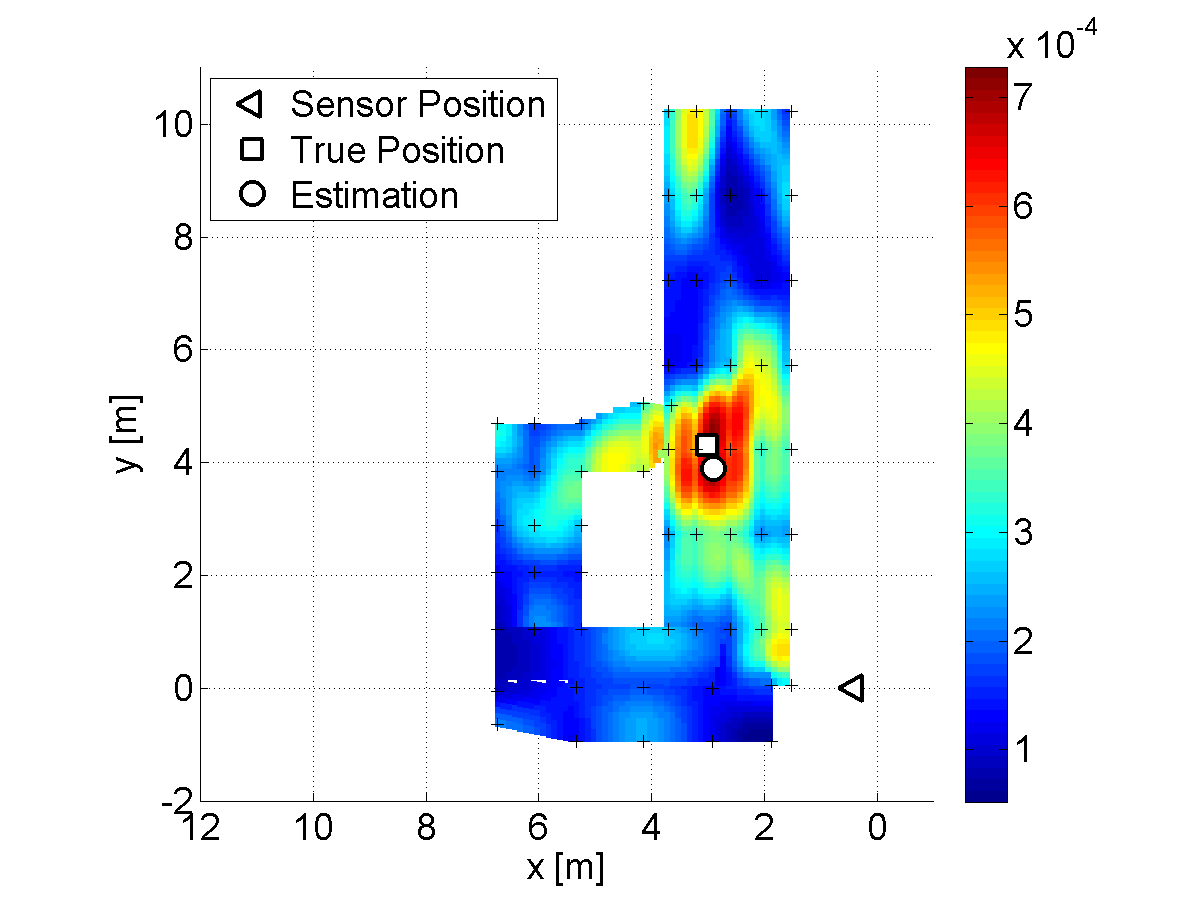
\includegraphics[trim =  15mm 0mm 15mm 0mm,clip,width = 0.46\columnwidth]{AOL_Figure3.png} % PDF
  }
  \subfigure[$k=51$ (NFOV)]{
    \label{fig:a4}
    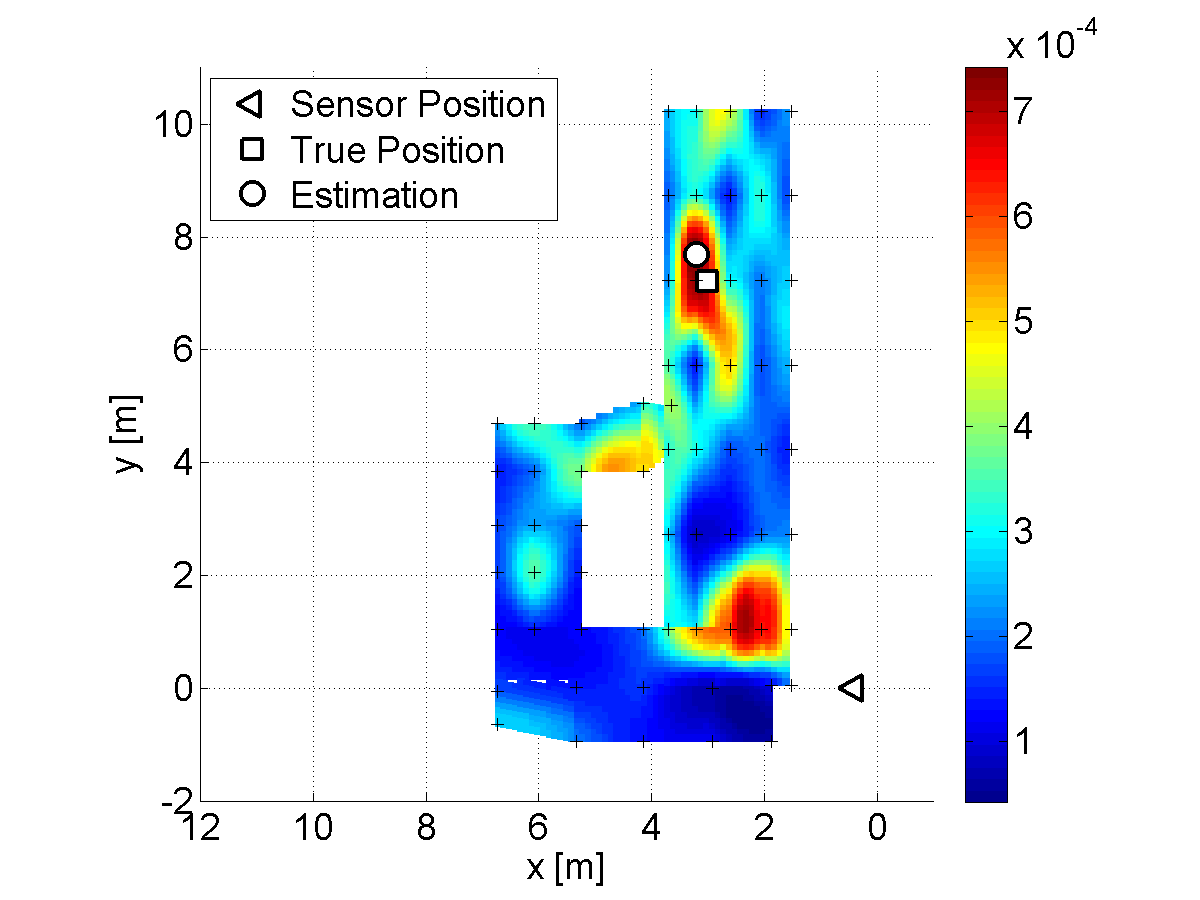
\includegraphics[trim =  15mm 0mm 15mm 0mm,clip,width = 0.46\columnwidth]{AOL_Figure4.png} % PDF
  }
	\caption{Acoustic observation likelihoods}
	\label{fig:acoustic likelihoods}
\end{figure}

The effectiveness of the proposed acoustic sensing technique is further understood comparatively by seeing optical observation likelihoods in Figure~{\ref{fig:optical likelihoods}}.  \thl{The optical sensor can identify the target accurately when it is within the FOV in Fig. {\ref{fig:o1}}.  The observation likelihood with the target outside the FOV in Fig. {\ref{fig:o2}}-{\ref{fig:o4}} can however provide no localization capability on the target. The likelihood of the target anywhere in NFOV is equally distributed with no specific estimation of the target position.}  Finally, Figure~\ref{fig:joint likelihoods} shows the joint optical/ acoustic observation likelihoods.  It is seen that the joint observation likelihoods most narrow down the possible target locations by detecting the target dominantly with the optical observation likelihood when the target is within the FOV and with the acoustic observation likelihood when the target is outside the FOV.  The wrong computation at the 7th step, however, remains and necessitates RBE for target estimation.  

\begin{figure}[ht]
	\centering
  \subfigure[$k=1$ (FOV)]{
    \label{fig:o1}
    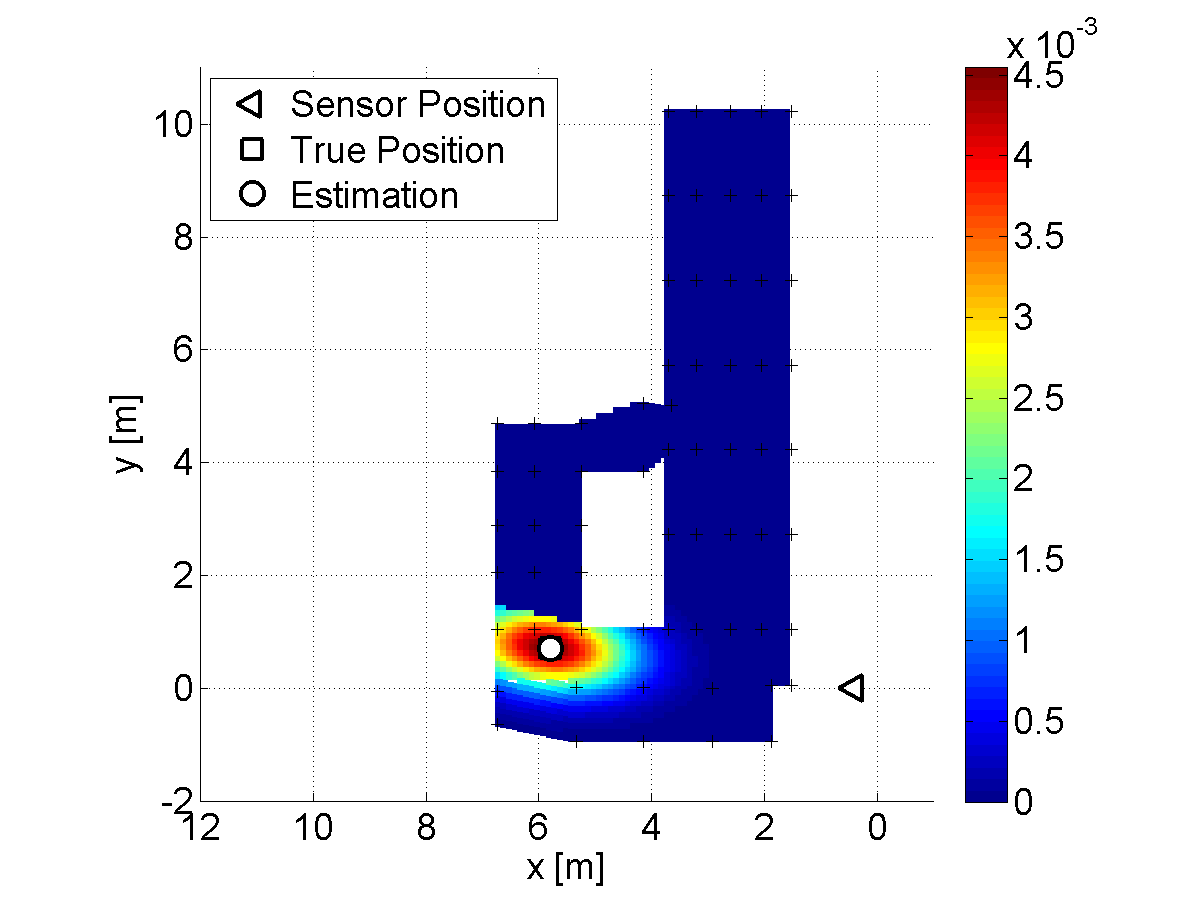
\includegraphics[trim = 15mm 0mm 15mm 0mm,clip,width = 0.46\columnwidth]{OOL_Figure1.png} % PDF
  }
  \subfigure[$k=7$ (NFOV)]{
    \label{fig:o2}
    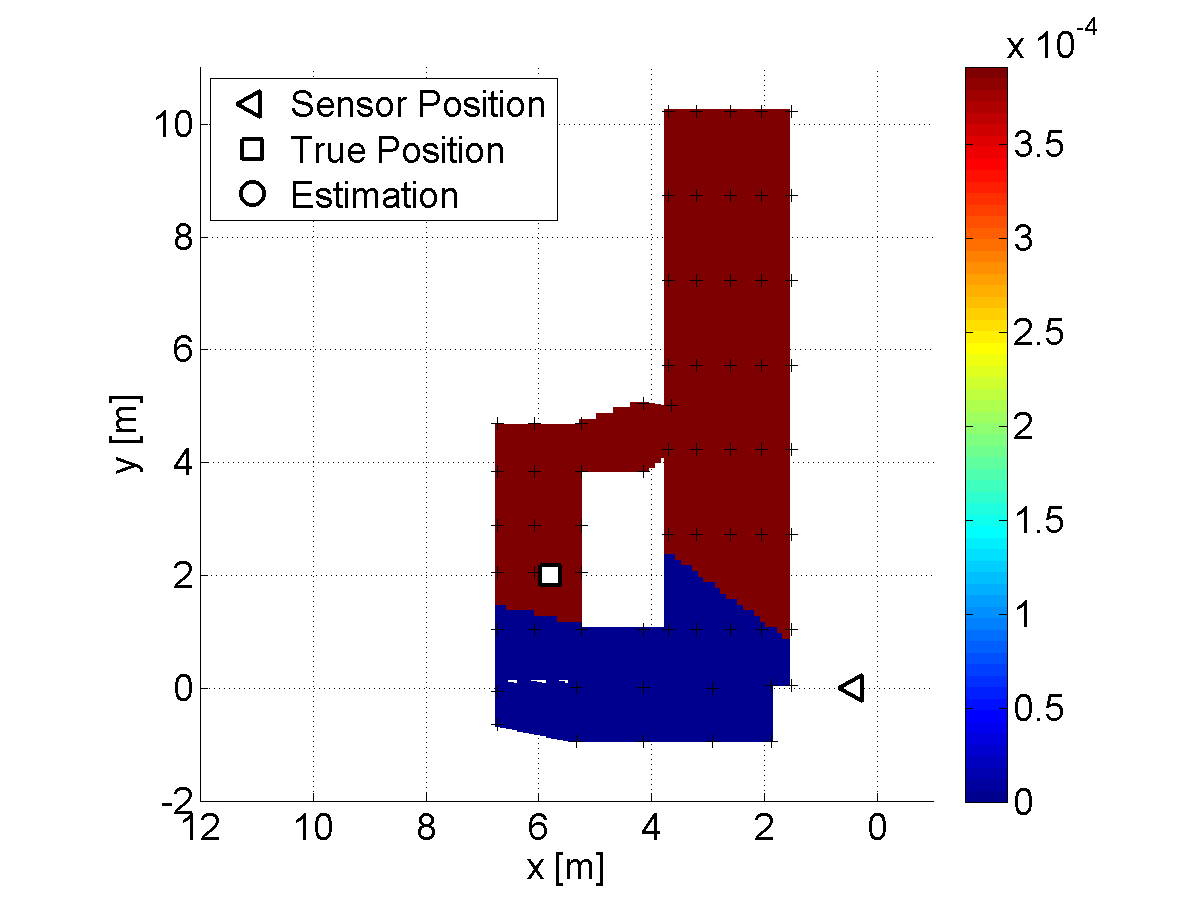
\includegraphics[trim = 15mm 0mm 15mm 0mm,clip,width = 0.46\columnwidth]{OOL_Figure2.png} % PDF
  }
  \subfigure[$k=35$ (NFOV)]{
    \label{fig:o3}
    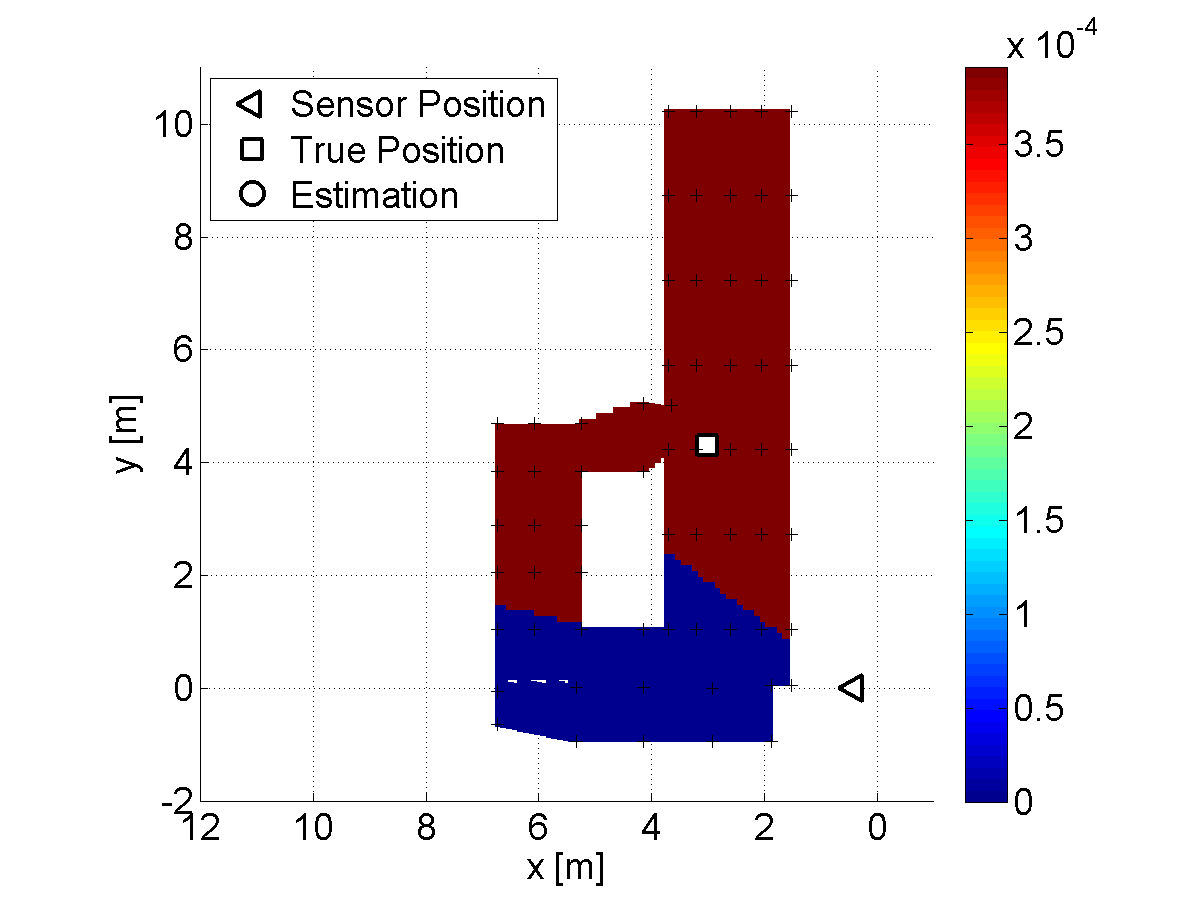
\includegraphics[trim = 15mm 0mm 15mm 0mm,clip,width = 0.46\columnwidth]{OOL_Figure3.png} % PDF
  }
  \subfigure[$k=51$ (NFOV)]{
    \label{fig:o4}
    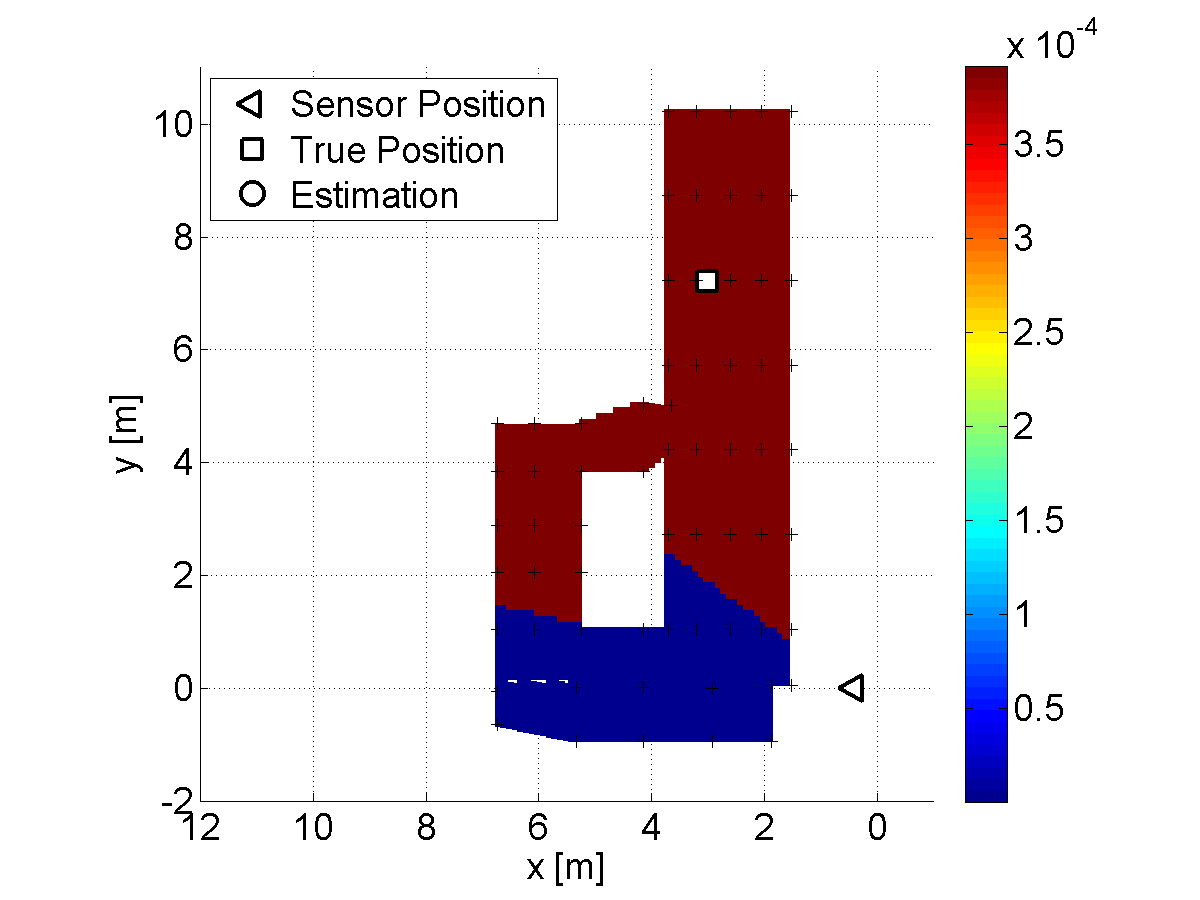
\includegraphics[trim = 15mm 0mm 15mm 0mm,clip,width = 0.46\columnwidth]{OOL_Figure4.png} % PDF
  }
	\caption{Optical observation likelihoods}
	\label{fig:optical likelihoods}
\end{figure}

\begin{figure}[ht]
	\centering
  \subfigure[$k=1$ (FOV)]{
    \label{fig:j1}
    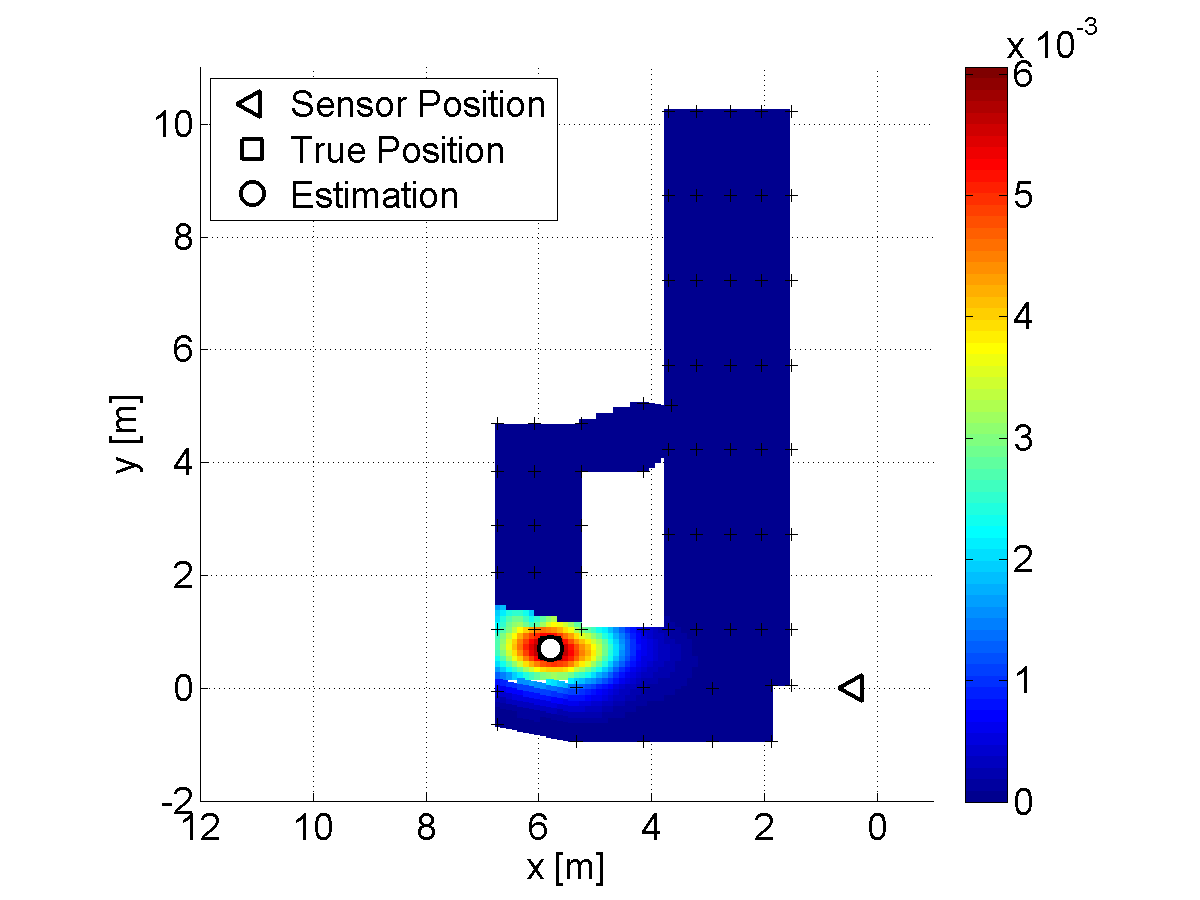
\includegraphics[trim = 15mm 0mm 15mm 0mm,clip,width = 0.46\columnwidth]{JOAO_Figure1.png} % PDF
  }
  \subfigure[$k=7$ (NFOV)]{
    \label{fig:j2}
    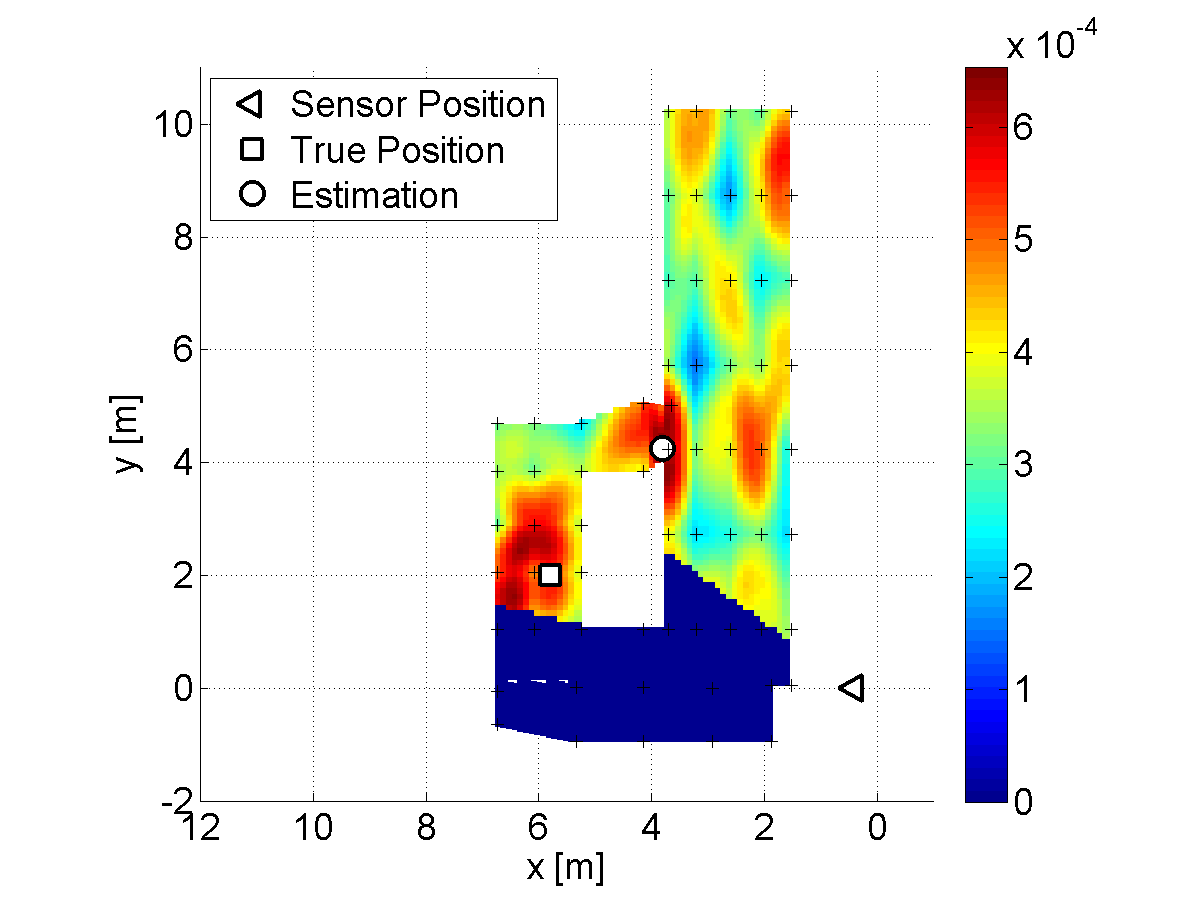
\includegraphics[trim = 15mm 0mm 15mm 0mm,clip,width = 0.46\columnwidth]{JOAO_Figure2.png} % PDF
  }
  \subfigure[$k=35$ (NFOV)]{
    \label{fig:j3}
    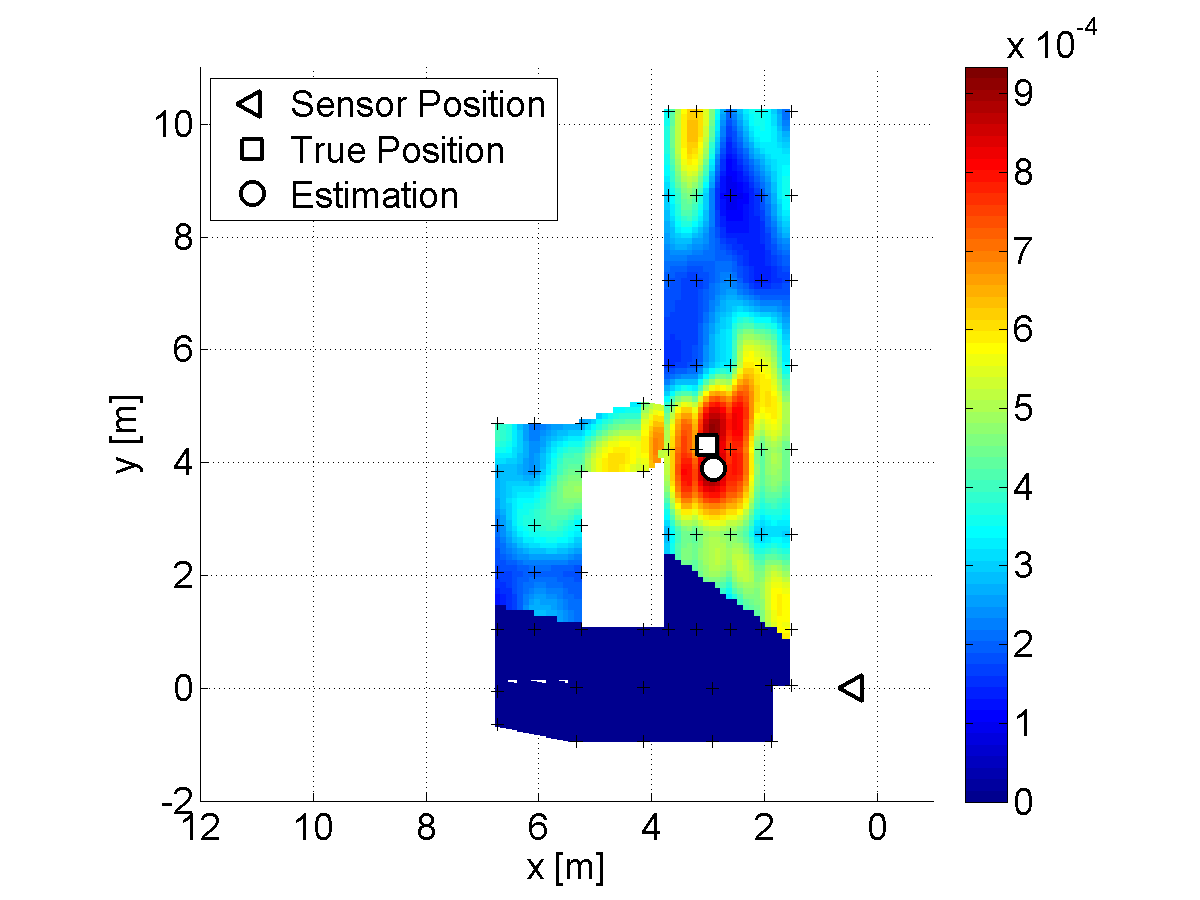
\includegraphics[trim = 15mm 0mm 15mm 0mm,clip,width = 0.46\columnwidth]{JOAO_Figure3.png} % PDF
  }
  \subfigure[$k=51$ (NFOV)]{
    \label{fig:j4}
    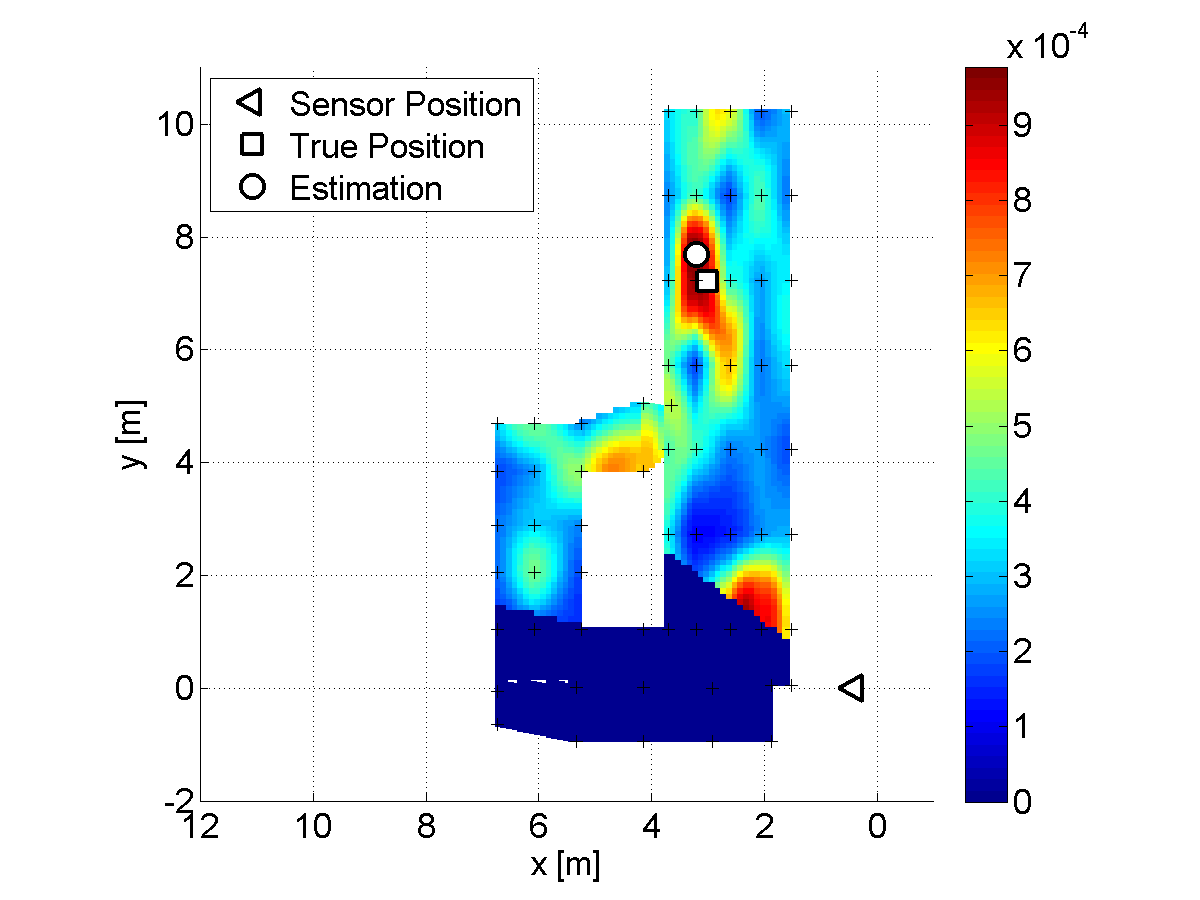
\includegraphics[trim = 15mm 0mm 15mm 0mm,clip,width = 0.46\columnwidth]{JOAO_Figure4.png} % PDF
  }
	\caption{Joint optical/acoustic observation likelihoods}
	\label{fig:joint likelihoods}
\end{figure}


%%%%%%%%%%%%%%%%%%%%%%%%%%%%%%%%%%%%%%%%
% Subsection
\subsubsection{RBE with Joint Optical/Acoustic Observation Likelihoods}
Having understood the limitation of the target detection with observations only in the last section, the effectiveness of the proposed RBE with the joint optical/acoustic observation likelihoods was investigated using the same test data.  Without knowing the target motion well, the target motion model was given by a random walk model assuming that the target is a human who could move to any direction with equal probability.  

Figure~\ref{fig:hybrid experiment} shows the target belief estimated via RBE with the joint optical/acoustic observation likelihoods.  The result shows that the target position is well estimated with all the time steps including the 7th step where the joint observation likelihood did not detect the target with the highest peak.  Because the target was initially observed by the optical sensor, strong and accurate prior belief was constructed.  Since the prior knowledge is updated by prediction with the random walk model and correction with the joint observation likelihood, the proposed approach can eliminate wrong detections and estimate the target position near the true position.  

\begin{figure}[ht]
	\centering
  \subfigure[$k=1$ (FOV)]{
    \label{fig:12-1}
    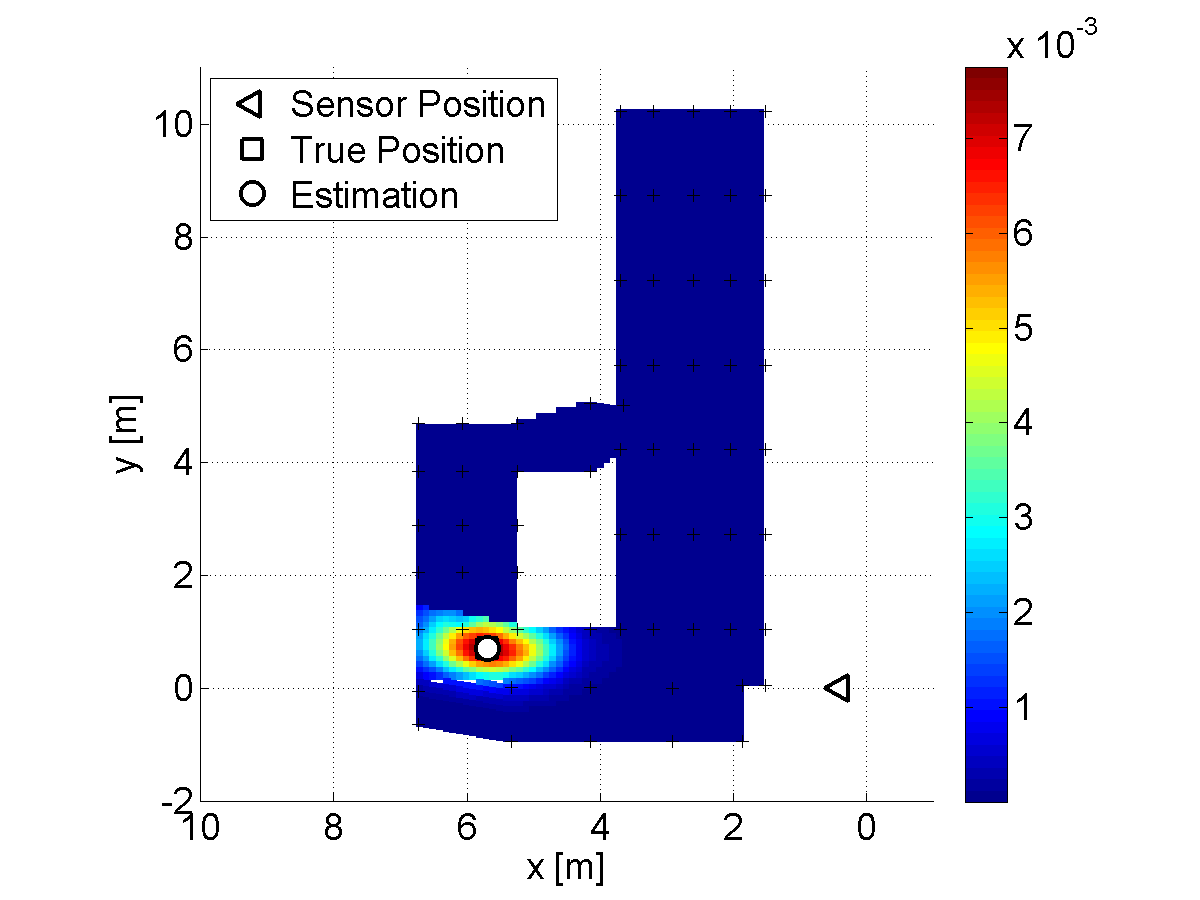
\includegraphics[trim = 15mm 0mm 15mm 0mm,clip,width = 0.46\columnwidth]{POA_Figure1.png} % PDF
  }
  \subfigure[$k=7$ (NFOV)]{
    \label{fig:12-7}
    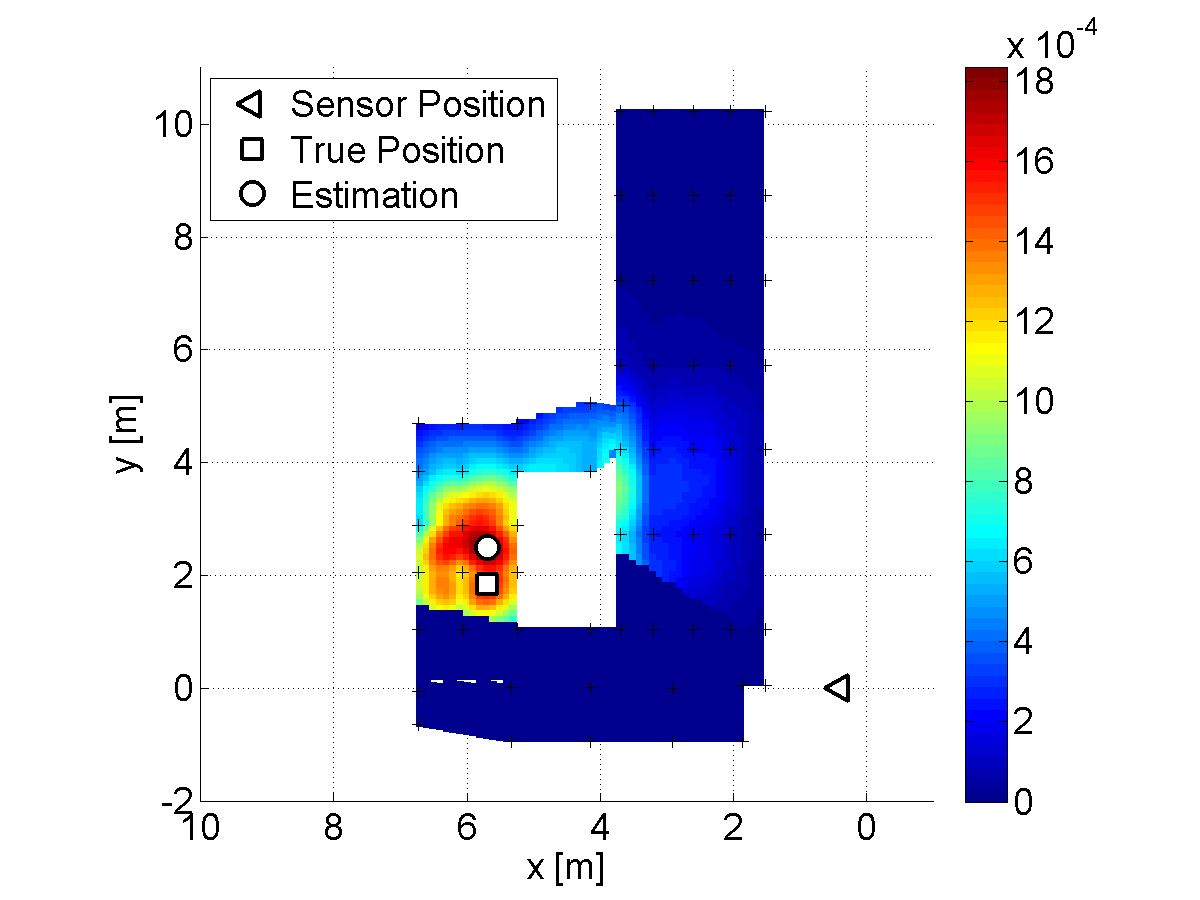
\includegraphics[trim = 15mm 0mm 15mm 0mm,clip,width = 0.46\columnwidth]{POA_Figure7.png} % PDF
  }
  \subfigure[$k=35$ (NFOV)]{
    \label{fig:12-35}
    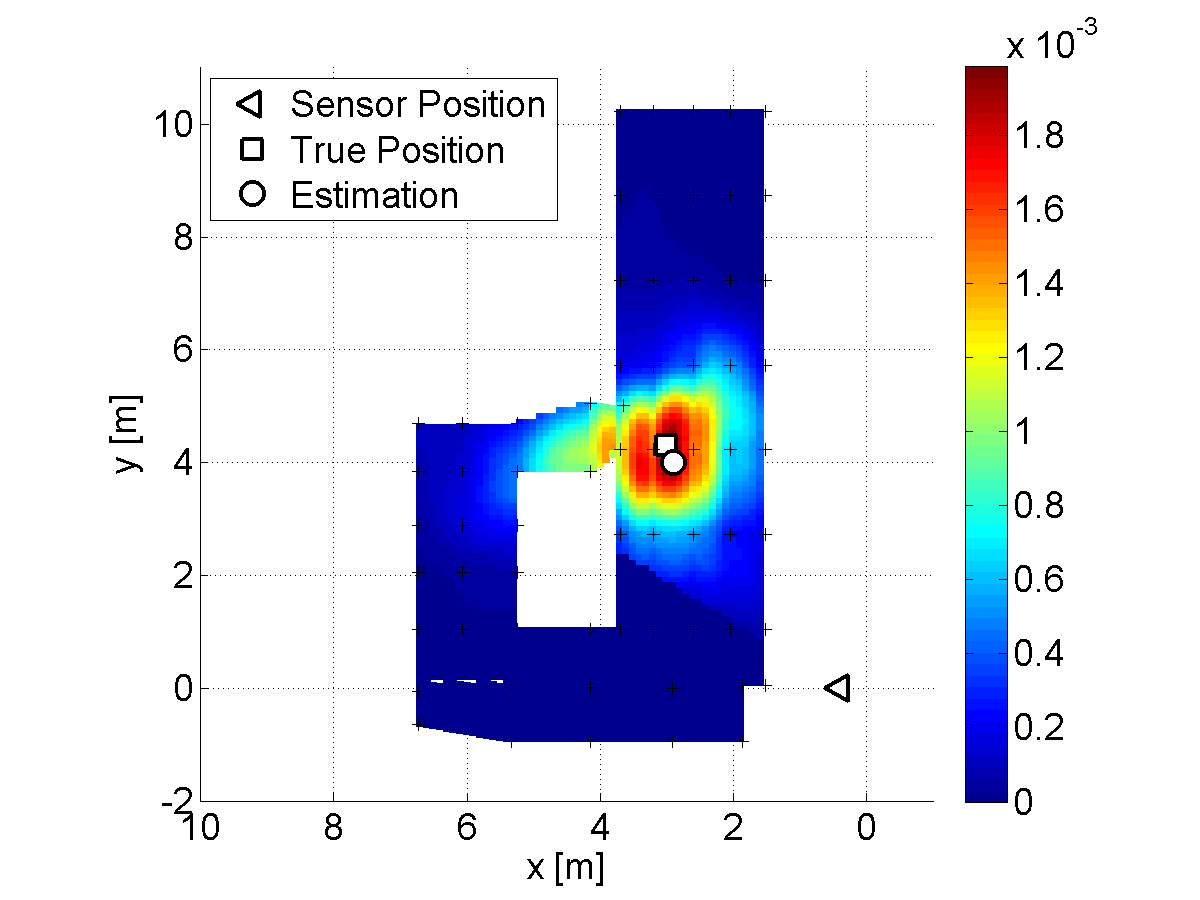
\includegraphics[trim = 15mm 0mm 15mm 0mm,clip,width = 0.46\columnwidth]{POA_Figure35.png} % PDF
  }
  \subfigure[$k=51$ (NFOV)]{
    \label{fig:12-51}
    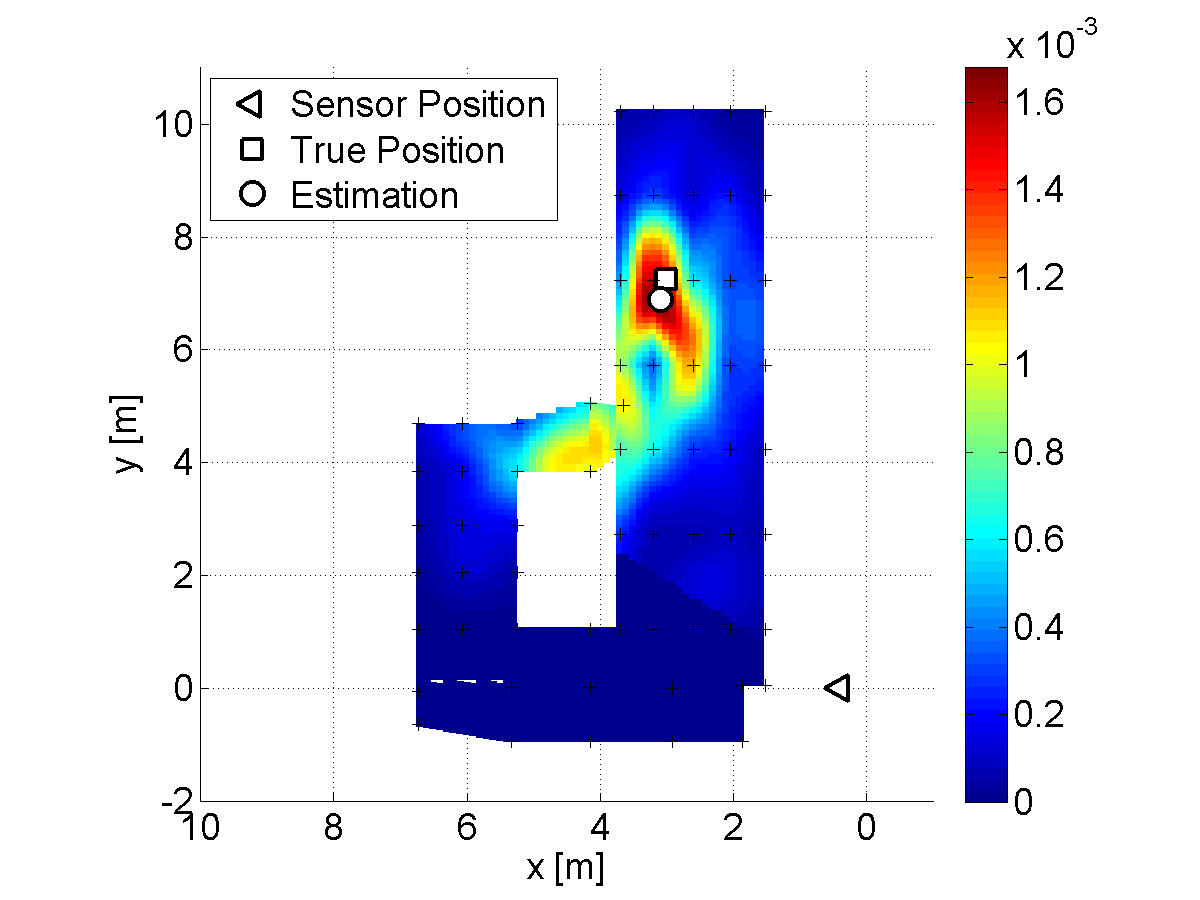
\includegraphics[trim = 15mm 0mm 15mm 0mm,clip,width = 0.46\columnwidth]{POA_Figure51.png} % PDF
  }
	\caption{Proposed optical/acoustic target estimation}
	\label{fig:hybrid experiment}
\end{figure}

Figure~\ref{fig:optical experiment} shows the target belief estimated conventionally with the optical observation likelihoods only to comparatively verify the effectiveness of the proposed approach.  The result with the optical observation likelihoods is seen to estimate the target position wrongly when the target is in the NFOV.  Because an inaccurate random-walk motion model is used, the target is estimated continuously at the location where it was lost.  Finally, Figure~\ref{fig:quantitative} shows the results quantitatively evaluating the performance of the proposed approach.  Figure~\ref{fig:error} shows the transition of the mean error of the estimated target position from the true position whereas the transition of the Kullback-Leibler (KL) divergence is exhibited in Figure~\ref{fig:kl}.  The error transition indicates that the proposed approach maintains error within 1 m even when the target has not been lost from the FOV for some time whilst the conventional RBE with optical observation likelihoods increases the error with high gradient.  The KL divergence transition also shows this behavior, indicating that the proposed approach maintains target information with the use of the acoustic sensor.  

\begin{figure}[ht]
	\centering
  \subfigure[$k=1$ (FOV)]{
    \label{fig:13-1}
    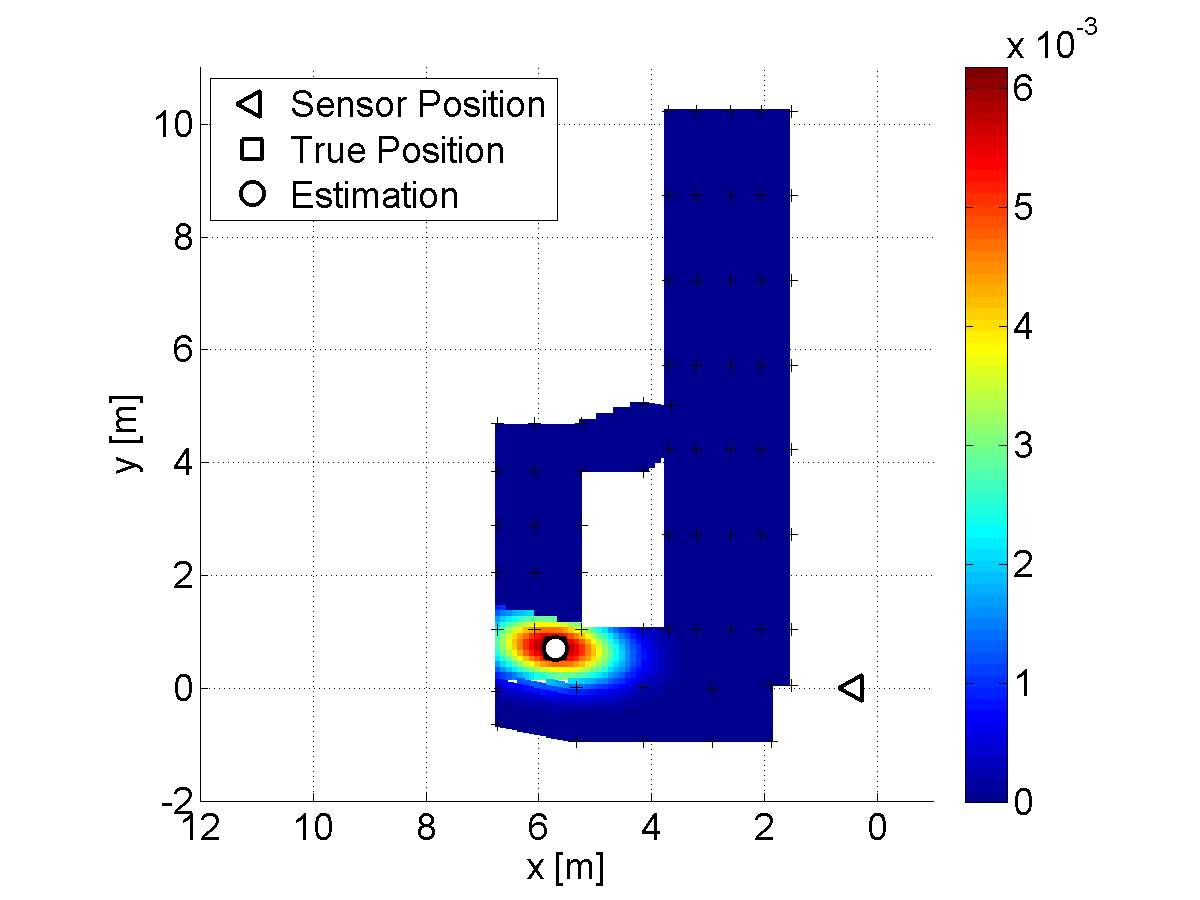
\includegraphics[trim = 15mm 0mm 15mm 0mm,clip,width = 0.46\columnwidth]{COT_Figure1.png} % PDF
  }
  \subfigure[$k=7$ (NFOV)]{
    \label{fig:13-7}
    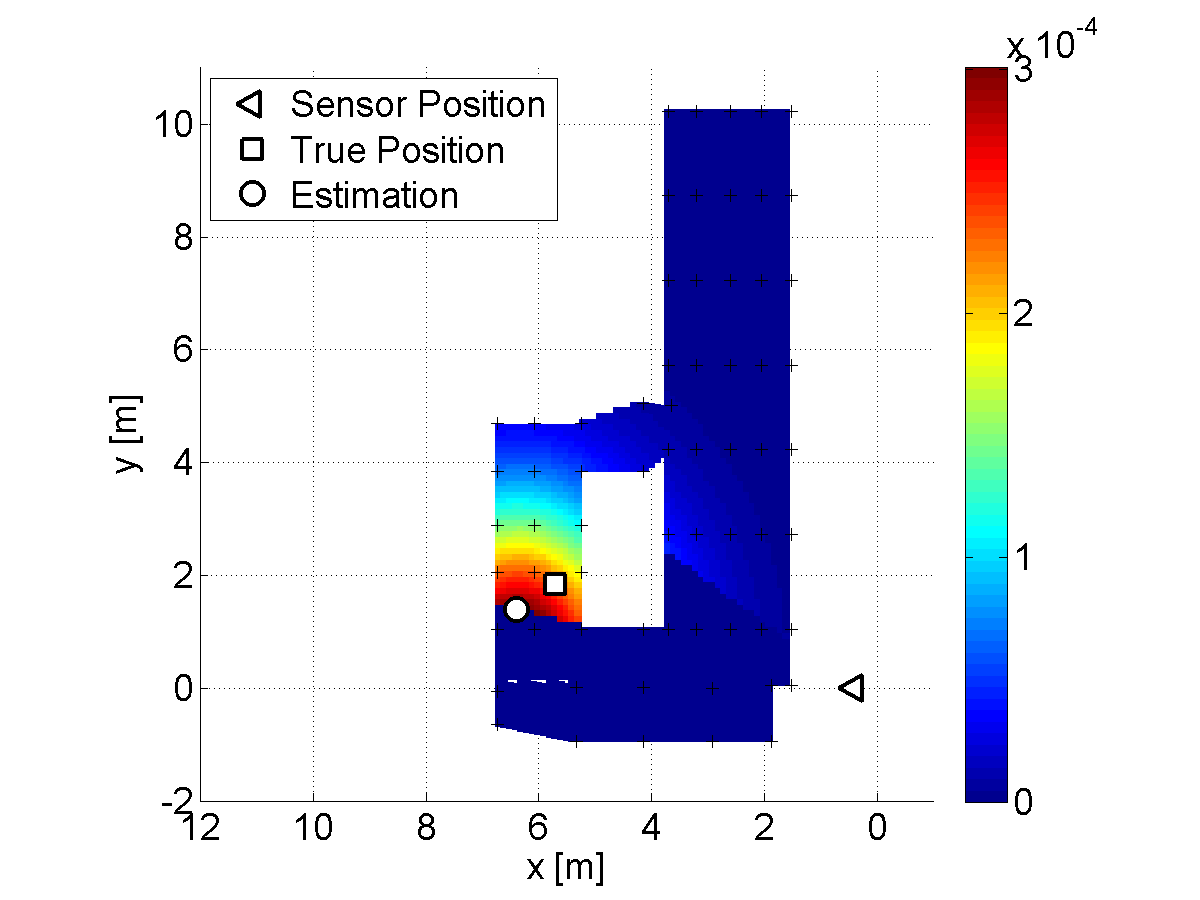
\includegraphics[trim = 15mm 0mm 15mm 0mm,clip,width = 0.46\columnwidth]{COT_Figure7.png} % PDF
  }
  \subfigure[$k=35$ (NFOV)]{
    \label{fig:13-35}
    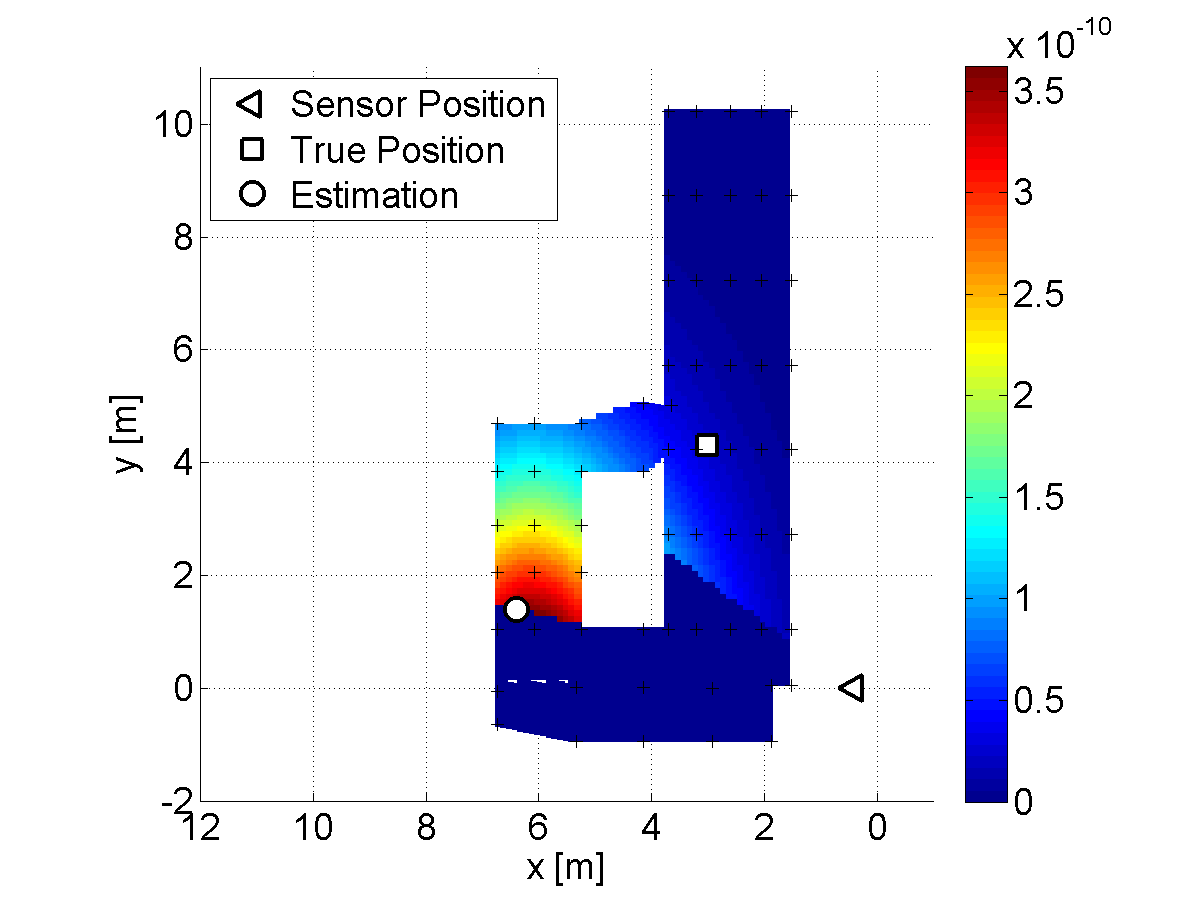
\includegraphics[trim = 15mm 0mm 15mm 0mm,clip,width = 0.46\columnwidth]{COT_Figure35.png} % PDF
  }
  \subfigure[$k=51$ (NFOV)]{
    \label{fig:13-51}
    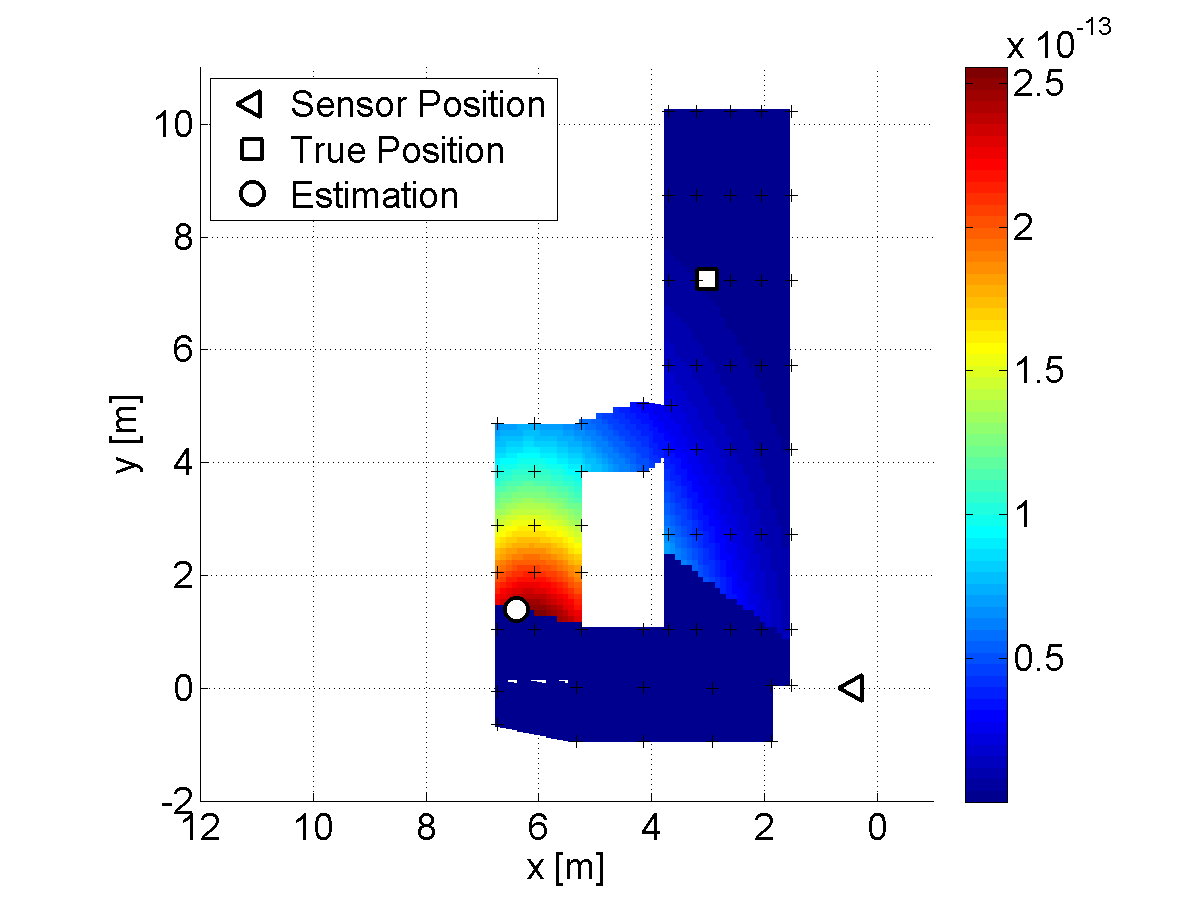
\includegraphics[trim = 15mm 0mm 15mm 0mm,clip,width = 0.46\columnwidth]{COT_Figure51.png} % PDF
  }
	\caption{Conventional optical target estimation}
	\label{fig:optical experiment}
\end{figure}

\begin{figure}[ht]
	\centering
  \subfigure[Error vs time step]{
    \label{fig:error}
    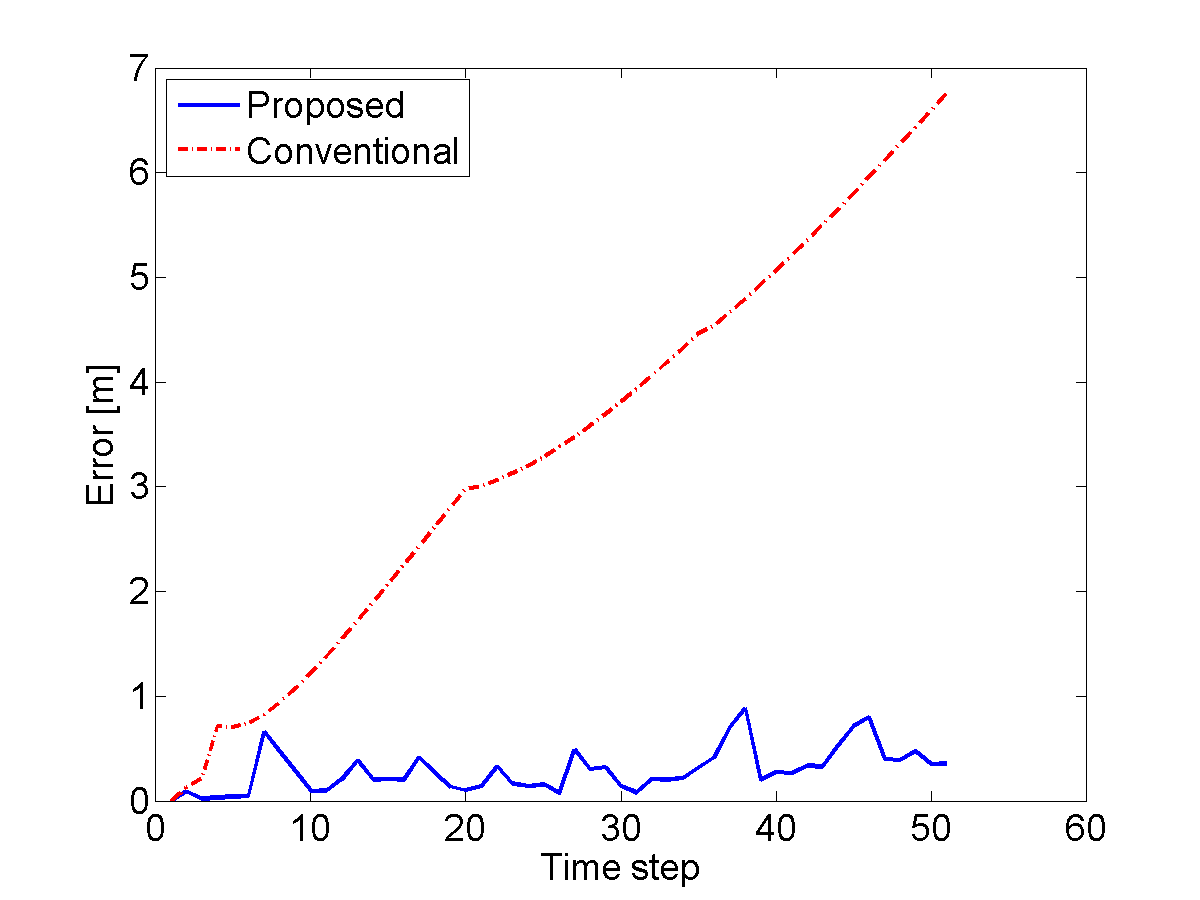
\includegraphics[trim = 0mm 0mm 15mm 0mm,clip,width = 0.46\columnwidth]{proposed_Error.png} % PDF
  }
  \subfigure[KL divergence vs time step]{
    \label{fig:kl}
    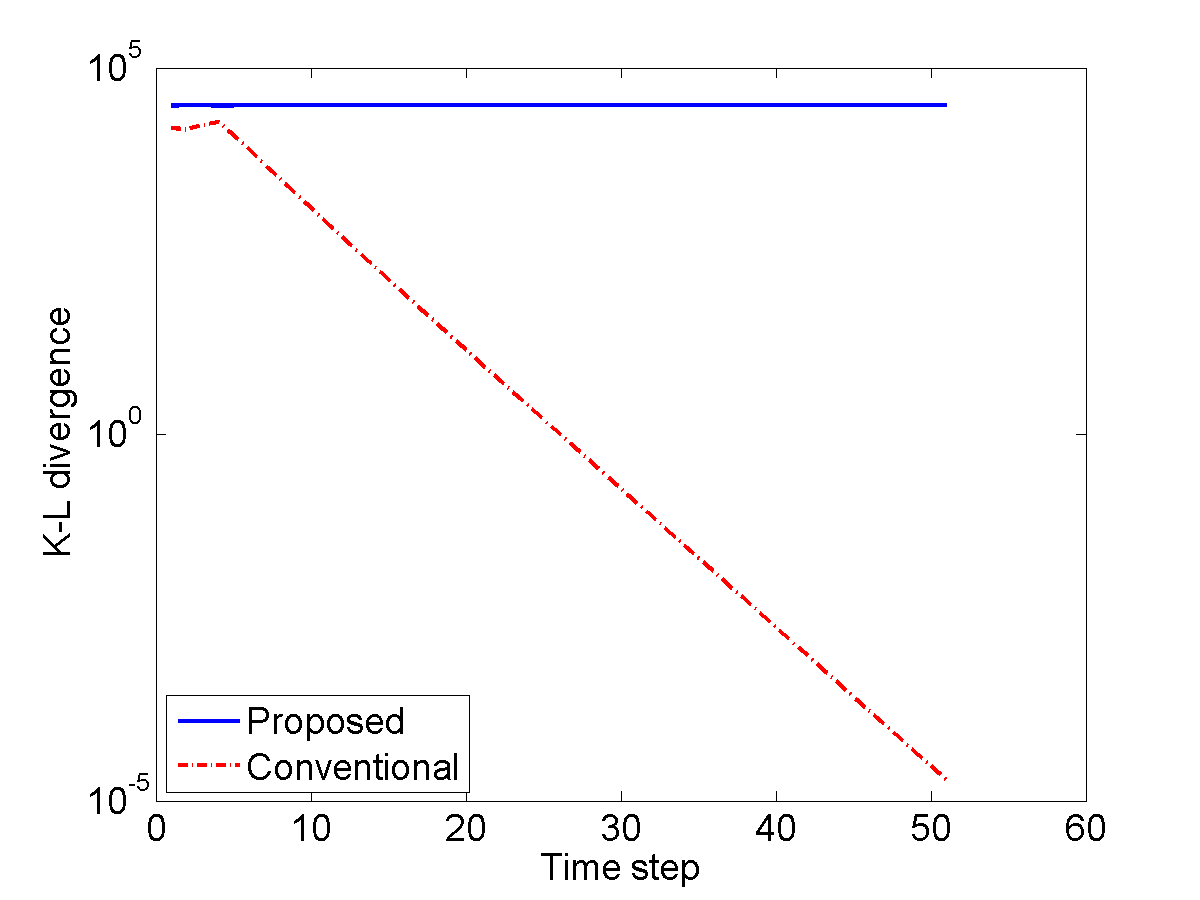
\includegraphics[trim = 0mm 0mm 15mm 0mm,clip,width = 0.46\columnwidth]{proposed_KLD.png} % PDF
  }
	\caption{Quantitative analysis}
	\label{fig:quantitative}
\end{figure}

%%%%%%%%%%%%%%%%%%%%%%%%%%%%%%%%%%%%%%%%%%%%%%%%%%%%%%%%%%%%%%%%%%%%%%%%%%%%%%%%
% SECTION
%%%%%%%%%%%%%%%%%%%%%%%%%%%%%%%%%%%%%%%%%%%%%%%%%%%%%%%%%%%%%%%%%%%%%%%%%%%%%%%%
\section{Conclusions}
\label{sec:conclusions}
This paper has presented a NFOV target estimation approach which incorporates optical and acoustic sensors.  The proposed approach performs RBE with joint optical/acoustic observation likelihoods.  Although the acoustic observation likelihood could be multi-modal with high uncertainty, the target belief updated in the past with sharply unimodal optical likelihoods effectively acts as strong prior knowledge and enables accurate NFOV target estimation.  A technique to construct an observation likelihood using an acoustic sensor composed of two microphones has also been proposed.  The acoustic observation likelihood is created by correlating the ILD of the new acoustic observation with the ILDs collected in advance.   

The first experiment studied the capability and limitation of the proposed acoustic sensing technique by parametrically changing the complexity of the environment.  It has been found that the proposed technique can identify the location of a NLOS target but with limited accuracy particularly when the complexity of the environment is severe.  The applicability of the proposed RBE approach with joint optical/acoustic observation likelihoods to the estimation of a NFOV target in a complex practical environment was the investigated as the second experiment.  The result shows that the target position is well estimated at all the time steps even when the joint observation likelihood does not identify the target location well due to the use of prediction with a motion model and strong prior belief constructed with the past optical observation.  

The paper has demonstrated the new concept for NFOV target estimation, and many challenges are still open for future study.  One of the improvements to the approach is the enhancement of acoustic sensing by incorporating the interaural time difference (ITD) and the interaural phase difference (IPD) as well as the use of non-white noise sound so that the approach could be used for various applications.  Other ongoing work includes the implementations of the proposed approach to the mobile sensor platform and to the infrastructure.  The proposed approach will can be used for various practical applications including home security, home heath care and urban search-and-rescue by the extension.  
\bibliography{reference/cite_cur}
\bibliographystyle{abbrv}

%\appendix
%\section*{Appendix}
%\subsection*{Nomenclature}

%\begin{itemize}[label={},leftmargin=1.5cm]
%    \item[$\Vxbp{k}{t}$]{state of the target at time step $k$}
%    \item[$\Vubp{k}{t}$]{target control inputs}
%    \item[$\Vwbp{k}{t}$]{ system noise of the target}
%   	\item[$\tVxp{s}$]{state of the sensor}
%   	\item[$\tilde{\bs{}}$]{instance of $\bs{}$} 
%   	\item[$P_d\bs{\Vxbp{k}{t}|\tVxp{s}}$]{probability of detecting the target}
%   	\item[$\pVzbp{s_c}{k}{t}$]{target obseved from the optical sensor}
%   	\item[$\pVvbp{s_c}{k}{t}$]{observation noise}
%   	\item[$\emptyset$]{empty element}
%   	\\
%\end{itemize}


%\bibliographystyle{spbasic}      % %basic style, author-year citations
%\bibliographystyle{spmpsci}      % mathematics and physical sciences
%\bibliographystyle{spphys}       % APS-like style for physics
%\begin{thebibliography}{10}
%
%\bibitem{Bahl2000}
%P.~Bahl and V.~N. Padmanabhan.
%\newblock Radar: An in-building rf-based user location and tracking system.
%\newblock In {\em INFOCOM 2000. Nineteenth Annual Joint Conference of the IEEE
%  Computer and Communications Societies. Proceedings. IEEE}, volume~2, pages
%  775--784. Ieee, 2000.
%
%\bibitem{Bertinato2008}
%M.~Bertinato, G.~Ortolan, F.~Maran, R.~Marcon, A.~Marcassa, F.~Zanella,
%  M.~Zambotto, L.~Schenato, and A.~Cenedese.
%\newblock Rf localization and tracking of mobile nodes in wireless sensors
%  networks: Architectures, algorithms and experiments.
%\newblock 2008.
%
%\bibitem{cha06}
%Y.~Chan, W.~Tsui, H.~So, and P.~Ching.
%\newblock Time-of-arrival based localization under nlos conditions.
%\newblock {\em Vehicular Technology, IEEE Transactions on}, 55(1):17--24, 2006.
%
%\bibitem{Chen1999}
%P.~Chen.
%\newblock A non-line-of-sight error mitigation algorithm in location
%  estimation.
%\newblock In {\em Wireless Communications and Networking Conference, 1999.
%  WCNC. 1999 IEEE}, pages 316--320. IEEE, 1999.
%
%\bibitem{Dai2012}
%H.~Dai, Z.~Zhu, and X.~Gu.
%\newblock Multi-target indoor localization and tracking on video monitoring
%  system in a wireless sensor network.
%\newblock {\em Journal of Network and Computer Applications}, 2012.
%
%\bibitem{fur06}
%T.~Furukawa, F.~Bourgault, B.~Lavis, and H.~Durrant{\-}Whyte.
%\newblock Recursive bayesian search-and-tracking using coordinated uavs for
%  lost targets.
%\newblock In {\em Robotics and Automation, 2006. ICRA 2006. Proceedings 2006
%  IEEE International Conference on}, pages 2521--2526. IEEE, 2006.
%
%\bibitem{fur12}
%T.~Furukawa, L.~C. Mak, H.~Durrant{\-}Whyte, and R.~Madhavan.
%\newblock Autonomous bayesian search and tracking, and its experimental
%  validation.
%\newblock {\em Advanced Robotics}, 26(5-6):461--485, 2012.
%
%\bibitem{Gao2013}
%P.~Gao, W.~Shi, W.~Zhou, H.~Li, and X.~Wang.
%\newblock A location predicting method for indoor mobile target localization in
%  wireless sensor networks.
%\newblock {\em International Journal of Distributed Sensor Networks}, 2013,
%  2013.
%
%\bibitem{Gezici2008}
%S.~Gezici.
%\newblock A survey on wireless position estimation.
%\newblock {\em Wireless Personal Communications}, 44(3):263--282, 2008.
%
%\bibitem{Guvenc2009}
%I.~Guvenc and C.~Chong.
%\newblock A survey on toa based wireless localization and nlos mitigation
%  techniques.
%\newblock {\em Communications Surveys \& Tutorials, IEEE}, 11(3):107--124,
%  2009.
%
%\bibitem{Jankovic2005}
%N.~D. Jankovic and M.~D. Naish.
%\newblock Developing a modular active spherical vision system.
%\newblock In {\em Robotics and Automation, 2005. ICRA 2005. Proceedings of the
%  2005 IEEE International Conference on}, pages 1234--1239. IEEE, 2005.
%
%\bibitem{Jung2011}
%J.~Jung and H.~Myung.
%\newblock Indoor localization using particle filter and map-based nlos ranging
%  model.
%\newblock In {\em Robotics and Automation (ICRA), 2011 IEEE International
%  Conference on}, pages 5185--5190, 2011.
%
%\bibitem{Khoury2009}
%H.~M. Khoury and V.~R. Kamat.
%\newblock Evaluation of position tracking technologies for user localization in
%  indoor construction environments.
%\newblock {\em Automation in Construction}, 18(4):444--457, 2009.
%
%\bibitem{kum11}
%D.~Kimoto and M.~Kumon.
%\newblock On sound direction estimation by binaural auditory robots with
%  pinnae.
%\newblock 35th Meeting of Special Interest Group on AI Challenges, 2011.
%
%\bibitem{kim12}
%D.~Kimoto and M.~Kumon.
%\newblock Optimization of the ear canal position for sound localization using
%  interaural level difference.
%\newblock 36th Meeting of Special Interest Group on AI Challenges, 2012.
%
%\bibitem{kobilarov2006}
%M.~Kobilarov, G.~Sukhatme, J.~Hyams, and P.~Batavia.
%\newblock People tracking and following with mobile robot using an
%  omnidirectional camera and a laser.
%\newblock In {\em Robotics and Automation, 2006. ICRA 2006. Proceedings 2006
%  IEEE International Conference on}, pages 557--562. IEEE, 2006.
%
%\bibitem{lad04}
%A.~M. Ladd, K.~E. Bekris, A.~P. Rudys, D.~S. Wallach, and L.~E. Kavraki.
%\newblock On the feasibility of using wireless ethernet for indoor
%  localization.
%\newblock {\em IEEE Transactions on Robotics and Automation}, 20(3):555--559,
%  2004.
%
%\bibitem{ledwich04}
%L.~Ledwich and S.~Williams.
%\newblock Reduced sift features for image retrieval and indoor localisation.
%\newblock Citeseer.
%
%\bibitem{Liu2007}
%H.~Liu, H.~Darabi, P.~Banerjee, and J.~Liu.
%\newblock Survey of wireless indoor positioning techniques and systems.
%\newblock {\em Systems, Man, and Cybernetics, Part C: Applications and Reviews,
%  IEEE Transactions on}, 37(6):1067--1080, 2007.
%
%\bibitem{lu10}
%Y.~Lu and M.~Cooke.
%\newblock Binaural estimation of sound source distance via the
%  direct-to-reverberant energy ratio for static and moving sources.
%\newblock {\em Audio, Speech, and Language Processing, IEEE Transactions on},
%  18(7):1793--1805, 2010.
%
%\bibitem{Mak2009}
%L.~C. Mak and T.~Furukawa.
%\newblock Non-line-of-sight localization of a controlled sound source.
%\newblock In {\em Advanced Intelligent Mechatronics, 2009. AIM 2009. IEEE/ASME
%  International Conference on}, pages 475--480. IEEE, 2009.
%
%\bibitem{mau03}
%R.~Mauler.
%\newblock {\em Recent Developments in Cooperative Control and Optimizatio},
%  chapter Objective Functions for Bayesian Control-Theoretic Sensor Management,
%  II: MHC-Like Approximation, pages 273--316.
%\newblock Kluwer Academic Publishers, Norwell, MA, 2003.
%
%\bibitem{nakadai06}
%K.~Nakadai, H.~Nakajima, M.~Murase, S.~Kaijiri, K.~Yamada, T.~Nakamura,
%  Y.~Hasegawa, H.~G. Okuno, and H.~Tsujino.
%\newblock Robust tracking of multiple sound sources by spatial integration of
%  room and robot microphone arrays.
%\newblock In {\em Acoustics, Speech and Signal Processing, 2006. ICASSP 2006
%  Proceedings. 2006 IEEE International Conference on}, volume~4, pages IV--IV.
%  IEEE, 2006.
%
%\bibitem{nayar1997}
%S.~K. Nayar.
%\newblock Catadioptric omnidirectional camera.
%\newblock In {\em Computer Vision and Pattern Recognition, 1997. Proceedings.,
%  1997 IEEE Computer Society Conference on}, pages 482--488. IEEE, 1997.
%
%\bibitem{Ni2004}
%L.~M. Ni, Y.~Liu, Y.~C. Lau, and A.~P. Patil.
%\newblock Landmarc: indoor location sensing using active rfid.
%\newblock {\em Wireless networks}, 10(6):701--710, 2004.
%
%\bibitem{nod12}
%Y.~Noda and M.~Kumon.
%\newblock Sound source direction estimation in the median plane by two active
%  pinnae.
%\newblock 13th SICE System Integration Division Annual Conference, 2012.
%
%\bibitem{Prigge2004}
%E.~A. Prigge.
%\newblock {\em A positioning system with no line-of-sight restrictions for
%  cluttered environments}.
%\newblock PhD thesis, Stanford University, 2004.
%
%\bibitem{rib05}
%J.~Riba and A.~Urruela.
%\newblock A non-line-of-sight mitigation technique based on ml-detection.
%\newblock In {\em Proceedings of IEEE International Conference on Acoustic,
%  Speech and Signal Processing}, volume~2, pages 153--156, May 2005.
%
%\bibitem{sasaki09}
%Y.~Sasaki, S.~Kagami, and H.~Mizoguchi.
%\newblock Online short-term multiple sound source mapping for a mobile robot by
%  robust motion triangulation.
%\newblock {\em Advanced Robotics}, 23(1-2):145--164, 2009.
%
%\bibitem{sederberg2003}
%T.~W. Sederberg, J.~Zheng, A.~Bakenov, and A.~Nasri.
%\newblock T-splines and t-nurccs.
%\newblock In {\em ACM transactions on graphics (TOG)}, volume~22, pages
%  477--484. ACM, 2003.
%
%\bibitem{Seow2008}
%C.~K. Seow and S.~Y. Tan.
%\newblock Non-line-of-sight localization in multipath environments.
%\newblock {\em Mobile Computing, IEEE Transactions on}, 7(5):647--660, 2008.
%
%\bibitem{sva12}
%P.~Svaizer, A.~Brutti, and M.~Omologo.
%\newblock Environment aware estimation of the orientation of acoustic sources
%  using a line array.
%\newblock In {\em Signal Processing Conference (EUSIPCO), 2012 Proceedings of
%  the 20th European}, pages 1024--1028. IEEE, 2012.
%
%\bibitem{mic03}
%J.~Valin, F.~Michaud, J.~Rouat, and D.~L{\'e}tourneau.
%\newblock Robust sound source localization using a microphone array on a mobile
%  robot.
%\newblock In {\em Intelligent Robots and Systems, 2003.(IROS 2003).
%  Proceedings. 2003 IEEE/RSJ International Conference on}, volume~2, pages
%  1228--1233. IEEE, 2003.
%
%\bibitem{Wang2012}
%J.~Wang, Q.~Gao, Y.~Yu, H.~Wang, and M.~Jin.
%\newblock Toward robust indoor localization based on bayesian filter using
%  chirp-spread-spectrum ranging.
%\newblock {\em Industrial Electronics, IEEE Transactions on}, 59(3):1622--1629,
%  2012.
%
%\bibitem{Zhang2010}
%D.~Zhang, Y.~Yang, D.~Cheng, S.~Liu, and L.~M. Ni.
%\newblock Cocktail: an rf-based hybrid approach for indoor localization.
%\newblock In {\em Communications (ICC), 2010 IEEE International Conference on},
%  pages 1--5. IEEE, 2010.
%
%\end{thebibliography}
\end{document}

